\documentclass[a4paper,dvips,openright]{report}
\usepackage{svn-multi}
% Version control information:
\svnidlong
{$HeadURL: https://practicas-spss.googlecode.com/svn/trunk/practicas_spss.tex $}
{$LastChangedDate: 2010-09-27 16:37:11 +0200 (lun, 27 sep 2010) $}
{$LastChangedRevision: 3 $}
{$LastChangedBy: asalber $}
%\svnid{$Id: practicas_spss.tex 3 2010-09-27 14:37:11Z asalber $}
\pdfinfo{/CreationDate (D:\svnpdfdate)}
\svnRegisterAuthor{asalber}{Alfredo S\'anchez Alberca}

\usepackage[spanish]{babel}
\usepackage[utf8x]{inputenc}
\usepackage{type1cm}
\usepackage{amsmath}
\usepackage{array}
%\usepackage{macros}
\usepackage[usenames,dvipsnames]{pstricks}
\usepackage{pst-all,pstricks-add,pst-math,pst-plot,pst-infixplot,pst-xkey}
\usepackage{epsfig}
\usepackage{graphicx}
\usepackage{enumitem}
\usepackage{subfigure}
\usepackage[colorlinks=true]{hyperref}
\hypersetup{pdfauthor={Alfredo S\'anchez Alberca (asalber@ceu.es)}, pdftitle={Pr\'acticas de estad\'{\i}stica con SPSS}} 
\usepackage[margin=20pt, font=small, labelfont=bf, labelsep=endash]{caption}
\usepackage[top=3cm, bottom=3cm, left=2.54cm, right=2.54cm]{geometry}
\usepackage{fancyhdr}
\pagestyle{fancy}

\lhead{\textsc{Universidad San Pablo CEU}} \rhead{\textsl{\textsf{Departamento de Métodos Cuantitativos}}}
\renewcommand{\headrulewidth}{0pt}
\renewcommand{\floatpagefraction}{.8}
\renewcommand{\textfraction}{.1} 

% Formato del título de las prácticas
\usepackage[rigidchapters,explicit]{titlesec}
\setlength{\fboxsep}{5pt}
\setlength{\titulolength}{\textwidth}
\addtolength{\titulolength}{-2\fboxsep}
\addtolength{\titulolength}{-2\fboxrule}
\titleformat{\chapter}[display]
{\bfseries\sffamily}
{\filleft \mdseries \slshape \LARGE Práctica de Estadística con SPSS \Huge\thechapter}
{0.5ex}
{\colorbox{mygreen}{\parbox[t]{\titulolength}{\rule{0mm}{10mm}\Huge\sffamily\filleft\textcolor{white}{#1}}}}
\titleformat{\section}{\normalfont\Large\bfseries}{\arabic{section}}{1em}{#1}
\titleformat{\subsection}{\normalfont\large\bfseries}{\arabic{section}.\arabic{subsection}}{1em}{#1}
\titleformat{\subsubsection}{\normalfont\normalsize\bfseries}{\arabic{section}.\arabic{subsection}.\arabic{subsubsection}}{0.5em}{#1}
\titlespacing{\chapter}{0pt}{0pt}{30ex}
\titlespacing{\section}{0pt}{8ex}{4ex}


\makeatletter
\let\savees@listquot\es@listquot
\def\es@listquot{\protect\savees@listquot}
\makeatletter

\definecolor{coral}{rgb}{1,0.5,0.31}
\definecolor{royalblue1}{rgb}{0.28,0.46,1}
\definecolor{mygreen}{rgb}{0,0.8,0}

%----------------------------------------------------------------------------------------
%    COMMANDS FOR INDICATIONS
%----------------------------------------------------------------------------------------
\newcommand{\menu}[1]{\textsl{#1}}
\newcommand{\boton}[1]{\textsl{#1}}
\newcommand{\opcion}[1]{\textsl{#1}}
\newcommand{\campo}[1]{\textsl{#1}}
\newcommand{\comando}[1]{\texttt{#1}}
\newcommand{\variable}[1]{\textsf{\scriptsize #1}}
\newcommand{\resultado}[1]{\texttt{#1}}
\newcommand{\flecha}{\mbox{$\rightarrow$}}

\newcommand{\resetcounters}{\setcounter{page}{1} \setcounter{section}{0} \setcounter{footnote}{0} \setcounter{figure}{0} \setcounter{table}{0}}

\begin{document}
\begin{titlepage}
\vspace*{5cm}
\begin{center}
{\huge \bf PRÁCTICAS DE ESTADÍSTICA CON SPSS\par}
\vspace{0.5cm}
{\large \noindent \textbf{Autores}: \\
Santiago Angulo Díaz-Parreño (\url{sangulo@ceu.es})\\
José Miguel Cárdenas Rebollo (\url{cardenas@ceu.es})\\
Anselmo Romero Limón (\url{arlimon@ceu.es})\\
Alfredo Sánchez Alberca (\url{asalber@ceu.es})
}

\vspace{0.5cm}
{\large Curso 2012-2013}

\vspace{1cm}
 \includegraphics[scale=0.3]{img/logo_uspceu_01}
\end{center}
%  \vfill
%  \flushleft\sffamily
%  Version control information:\\
%  Head URL: \url{\svnmainurl}\\
%  Last changed date: \svndate\\
%  Last changes revision: \svnrev\\
%  Version: \svnFullRevision*{\svnrev}\\
%  Last changed by: \svnFullAuthor*{\svnauthor}\\
\end{titlepage}

\include{licencia}
\renewcommand{\thepage}{\roman{page}}
\setcounter{page}{1} 
\thispagestyle{plain}
\tableofcontents
\cleardoublepage
\renewcommand{\thepage}{\arabic{page}}
\setcounter{page}{1} 

% Version control information:
%$HeadURL: https://practicas-spss.googlecode.com/svn/trunk/introduccion_spss/introduccion_spss.tex $
%$LastChangedDate: 2010-09-27 16:37:11 +0200 (lun, 27 sep 2010) $
%$LastChangedRevision: 3 $
%$LastChangedBy: asalber $
%$Id: introduccion_spss.tex 3 2010-09-27 14:37:11Z asalber $

\chapter{Introducción a SPSS}

\section{Introducción}
La gran potencia de cálculo alcanzada por los ordenadores ha convertido a los mismos en poderosas herramientas al servicio de todas aquellas disciplinas que, como la estadística, requieren manejar un gran volumen de datos.
Actualmente, prácticamente nadie se plantea hacer un estudio estadístico serio sin la ayuda de un buen programa de análisis estadístico.

SPSS$^{\textsf{\textregistered}}$\renewcommand{\thefootnote}{\fnsymbol{footnote}}\footnote{Esta practica está basada en la versión 20.0 de SPSS$^{\textsf{\textregistered}}$ para Windows en español.} es uno de los programas de análisis estadísticos más utilizados, sobre todo en el ámbito de las ciencias biosanitarias.
\begin{center}
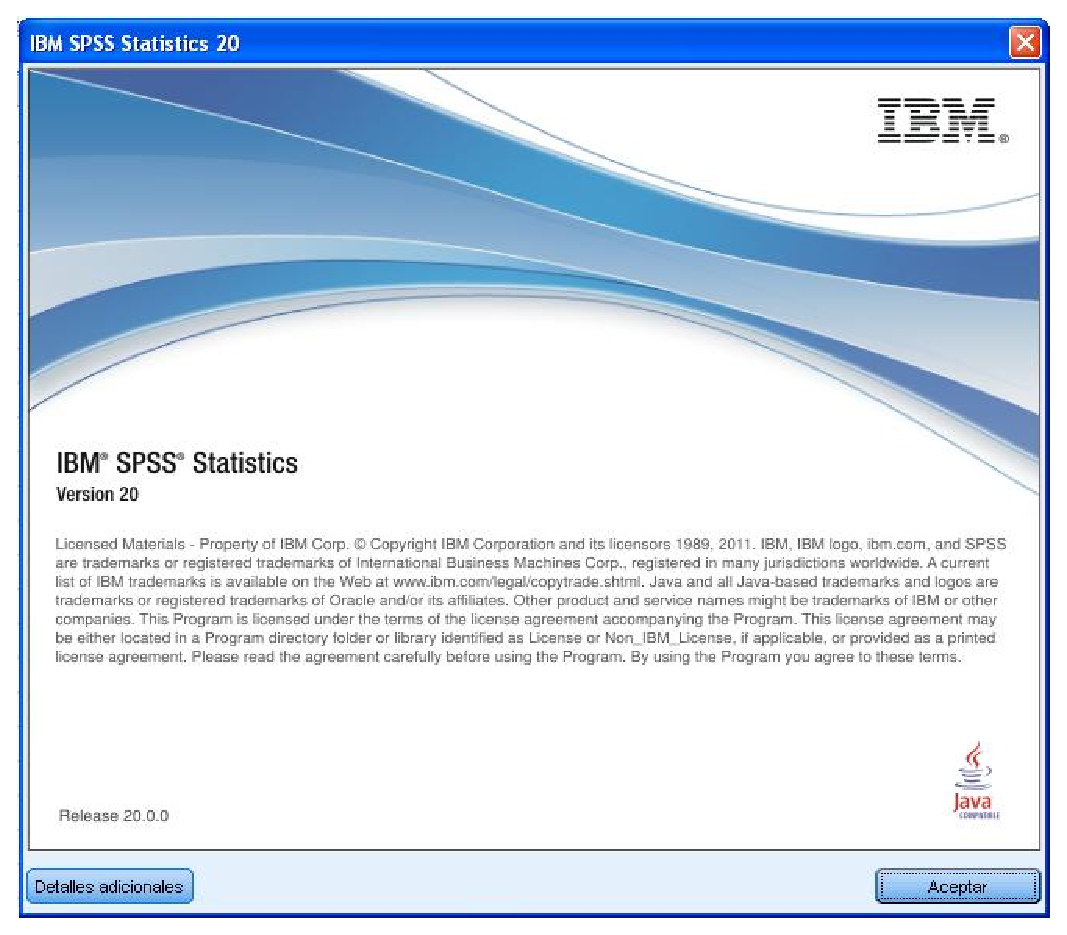
\includegraphics[scale=0.5]{introduccion_spss/img/portada}
\end{center}

El objetivo de esta práctica es introducir al alumno en la utilización de este programa, enseñándole a realizar las operaciones básicas más habituales. A lo largo de la práctica, los alumnos aprenderán a crear variables, introducir datos de las muestras, transformar variables, filtrar datos y fundir e importar archivos de datos.  


\section{Funciones básicas}
\subsection{Arranque}
Como cualquier otra aplicación de Windows, para arrancar el programa
hay que hacer click sobre la opción correspondiente del menú
\menu{Inicio\flecha Programas}, o bien sobre el icono de escritorio
\begin{center}
  
\includegraphics{introduccion_spss/img/icono}
\end{center}

Cuando el programa arranca, aparece la ventana del editor de datos (figura~\ref{g:vista_datos}).
\begin{figure}[h!]
\begin{center}
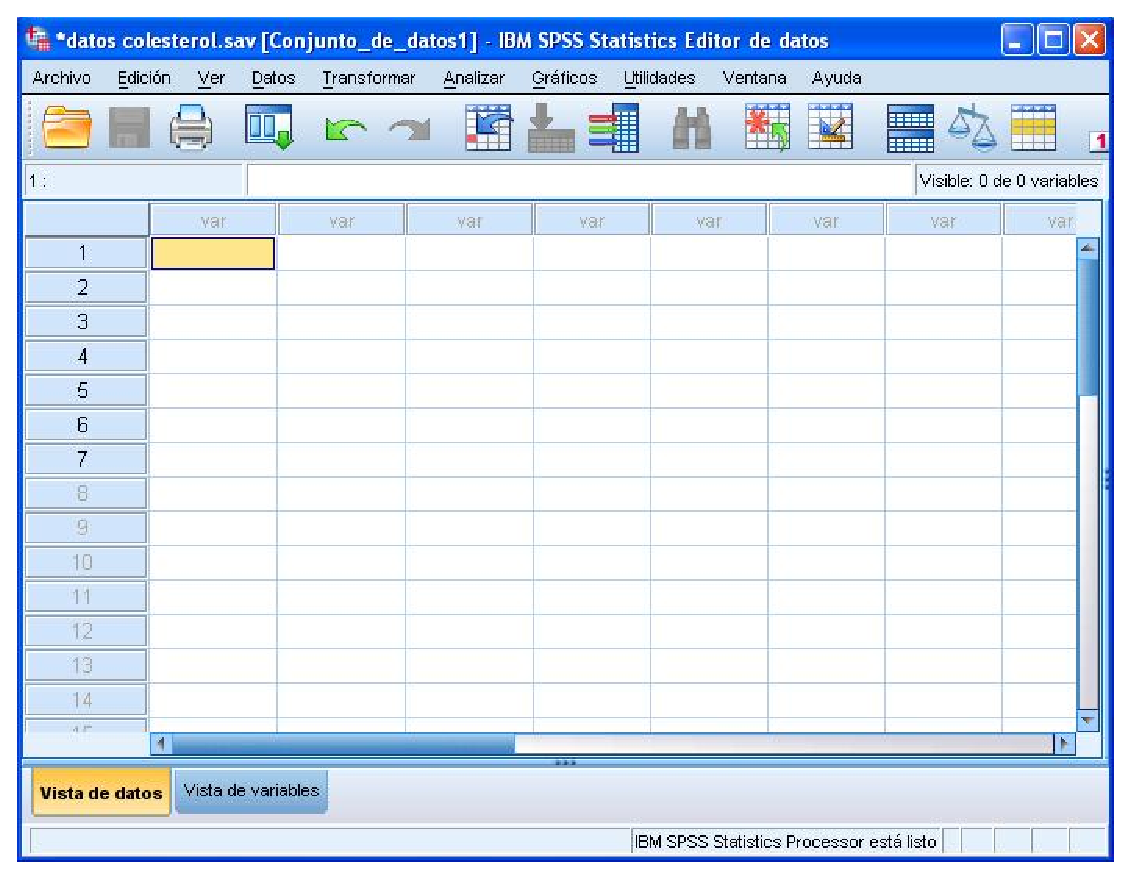
\includegraphics[scale=0.5]{introduccion_spss/img/vista_datos}
\caption{Ventana del editor de datos.}
\label{g:vista_datos}
\end{center}
\end{figure}
 
Como cualquier otra ventana de aplicación de Windows, la ventana del editor de datos tiene una barra de título, una barra de menús con las distintas funciones que puede hacer SPSS, entre ellas los análisis estadísticos de datos, una barra de botones que son atajos a las opciones más habituales de los menús, y una barra de estado en la parte inferior que nos indica lo que hace el programa en cada instante. Además, en la parte inferior aparecen dos pestañas que permiten pasar a la \opcion{Vista de datos} o a la \opcion{Vista de variables}.

\subsection{Introducción de datos}\label{s:introduccion_datos}
Para realizar cualquier análisis, la ventana del editor de datos debe contener la matriz de datos a analizar. Una vez que el usuario obtiene los datos muestrales, estos deben introducirse en esta ventana. Para ello, lo primero es definir las variables que se han considerado en el estudio. Cada variable se corresponderá con una columna de la matriz de datos. 

Para definir una variable debemos pasar a la \opcion{Vista de variables} haciendo click sobre la correspondiente pestaña (figura~\ref{g:vista_variables}). 

\begin{figure}[h!]
\begin{center}
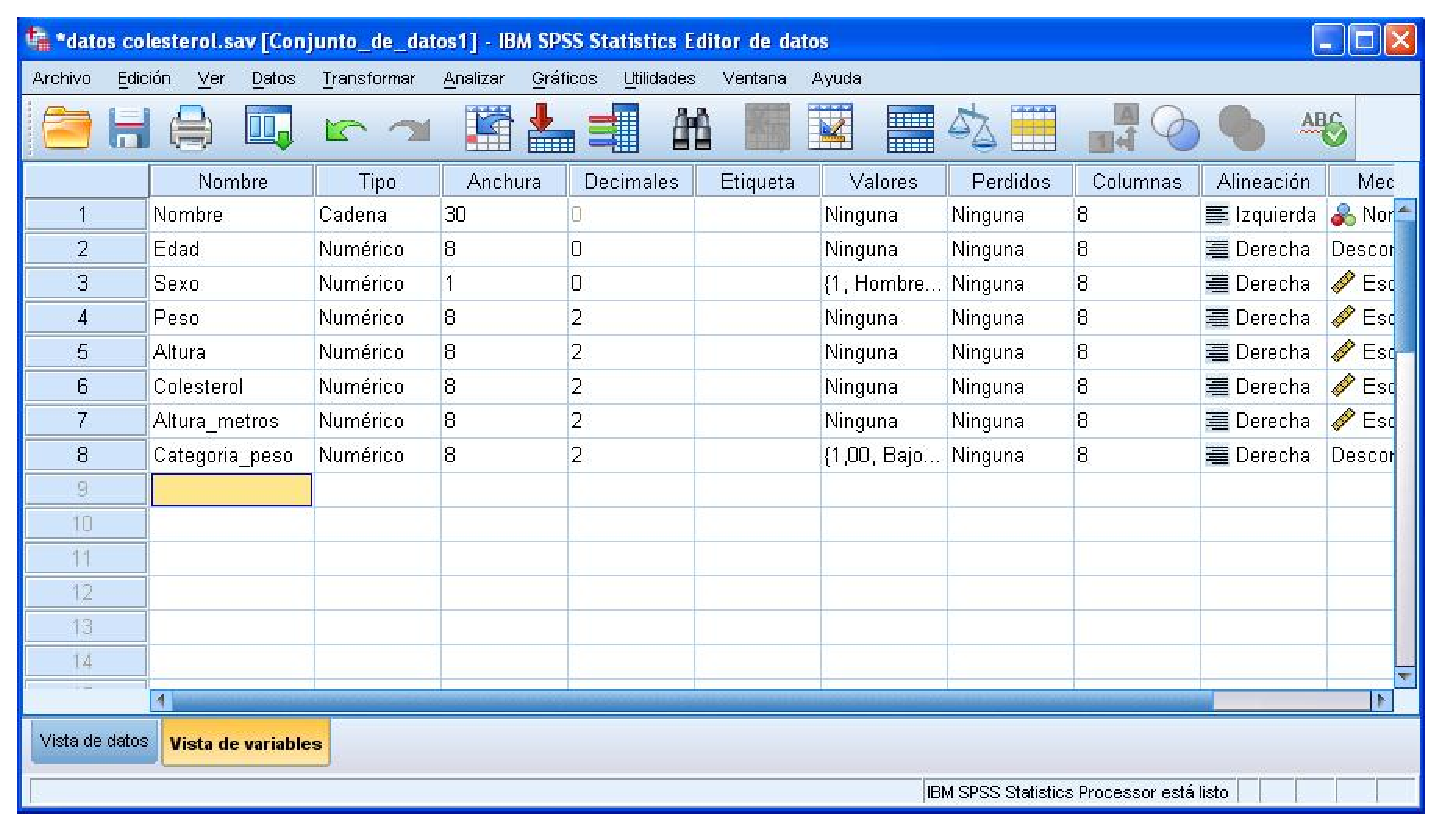
\includegraphics[scale=0.5]{introduccion_spss/img/vista_variables}
\caption{Vista de definición de variables.}
\label{g:vista_variables}
\end{center}
\end{figure}

En esta otra ventana, debemos definir cada variable en una fila, rellenando los siguientes campos:
\begin{description}
\item[Nombre] El nombre de la variable puede ser cualquier cadena de caracteres que comience por una letra y que no contenga espacios en blanco ni caracteres especiales como ?,¿,*, etc. Cada nombre de variable debe ser único y no se distingue entre mayúsculas y minúsculas. 
\item[Tipo] Los tipos más comunes son \texttt{Numérico} (formato numérico estándar), \texttt{Coma} (con comas de separación cada tres cifras y punto para la parte decimal), \texttt{Punto} (con puntos de separación cada tres cifras y coma para la parte decimal), \texttt{Notación Científica} (utiliza la E para la exponenciación), \texttt{Cadena} (para datos alfanuméricos) y \texttt{Fecha}.
\item[Anchura] Es el número máximo de caracteres que pueden tener los valores de la variable.
\item[Decimales] Para las variables numéricas es el número de cifras decimales que podrán escribirse.
\item[Etiqueta] Es una descripción de la variable. Si el nombre de la variable es suficientemente descriptivo se puede omitir. 
\item[Valores] Permite asignar etiquetas a los distintos valores que puede tomar la variable. No es obligatorio pero puede ser útil en algunos casos. 

Al hacer click sobre la casilla aparece un cuadro de diálogo para asignar etiquetas a valores. Para ello basta con escribir un valor en el cuadro de texto \opcion{Valor} y la correspondiente etiqueta en el cuadro de texto \opcion{Etiqueta}. Después hay que hacer click sobre el botón \boton{Añadir} y repetir los mismos pasos para todos los valores de la variable. Para finalizar hay que hacer click en el botón \boton{Aceptar}.
\item[Perdidos] Permite definir qué valores se utilizarán para representar los datos perdidos por el usuario. Es útil para distinguir datos que se han perdido por distintas causas. Por ejemplo, puede ser interesante distinguir el dato perdido correspondiente a un entrevistado que se niega a responder, del dato perdido debido a que la pregunta no le afectaba al entrevistado. Los valores de datos especificados como perdidos por el usuario se excluyen de la mayoría de los cálculos. 

Al hacer click sobre la casilla aparece un cuadro de diálogo donde deben indicarse los valores discretos que representarán valores perdidos (pueden introducirse hasta tres), o bien, el rango de valores que se representarán como valores perdidos. 

\item[Columnas] Permite especificar el ancho de la columna en la que se introducirán los datos correspondientes a la variable. 

\item[Alineación] Permite especificar la alineación de los datos correspondientes a la variable. Puede ser Izquierda, Derecha o Centrado. 

\item[Medida] Permite especificar el tipo de escala utilizada para medir la variable. Puede ser \opcion{Escala} cuando la variable es numérica y la escala es de intervalo, \opcion{Ordinal} cuando los valores de la variable representan categorías con un cierto orden o \opcion{Nominal} cuando los valores representan categorías sin orden.
\item[Rol] Permite especificar la función que una variable tiene en el análisis. Puede ser \opcion{entrada}, cuando se trata de una variable
independiente, \opcion{objetivo}, cuando es una variable dependiente, \opcion{ambos}, cuando la variable puede ser dependiente e
independiente, \opcion{ninguna} si la variable no tiene ninguna función asignada, \opcion{particion}, cuando la variable se utilizará para
dividir los datos en muestras separadas y \opcion{segmentar}, cuando se trata de una variable introducida para asegurar la compatibilidad en
SPSS.
\end{description}


Una vez definidas las variables se procede a introducir los datos de la muestra. Para ello hay que volver a la \opcion{Ventana de datos} haciendo click en la correspondiente pestaña. Ahora aparecerán en las cabeceras de columna los nombres de las variables definidas. Cada individuo de la muestra se corresponde con una fila de la matriz de datos. Para introducir el valor de una variable en un individuo determinado, nos situamos en la celda de la fila de dicho individuo y de la columna de la variable, bien haciendo click sobre la misma, o bien desplazándonos por la matriz de datos con las flechas de movimiento del cursor del teclado, y se teclea el valor seguido de la tecla \boton{Intro} (figura~\ref{g:matriz_datos}).

\begin{figure}[h!]
\begin{center}
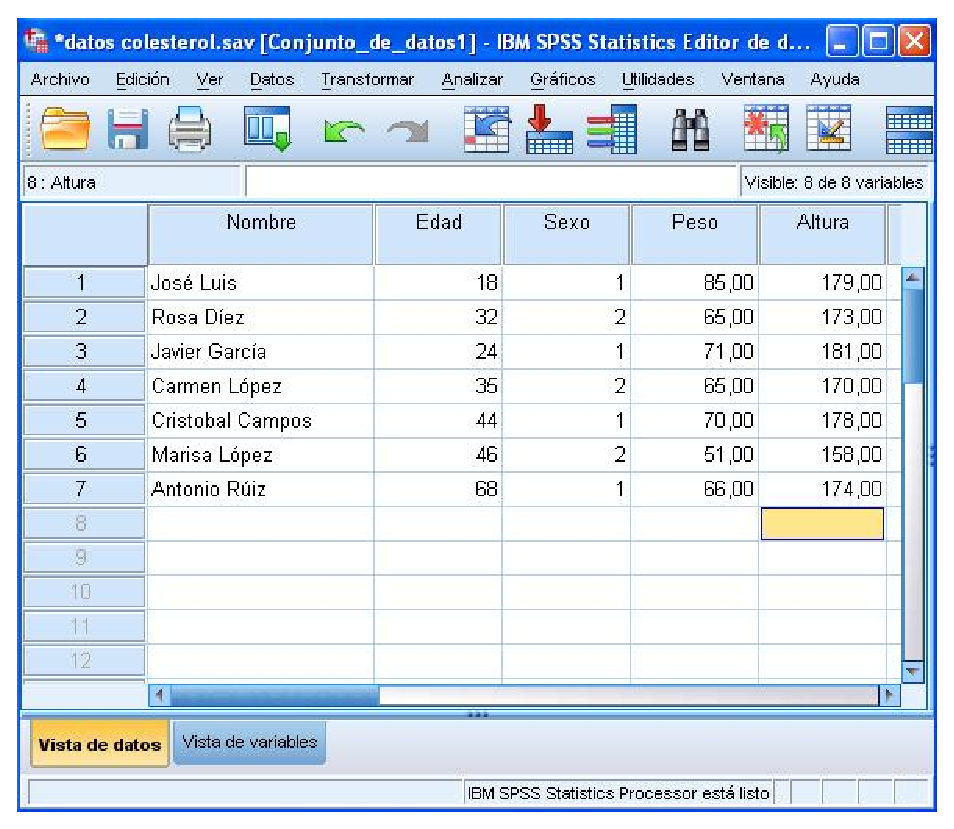
\includegraphics[scale=0.5]{introduccion_spss/img/matriz_datos}
\caption{Introducción de datos en la matriz de datos. Cada columna corresponde a una variable y cada fila a un individuo de la muestra.}
\label{g:matriz_datos}
\end{center}
\end{figure}

\subsection{Guardar datos}\label{s:guardar_datos}
Una vez introducidos los datos, conviene guardarlos en un fichero para no tener que volver a introducirlos en futuras sesiones. Para ello,
se selecciona el menú \menu{Archivo\flecha Guardar}. Si el fichero ya existe, se actualizará su información, y si no, aparecerá un cuadro de
diálogo en el que hay que introducir el nombre que queremos darle al fichero y la carpeta donde lo queremos ubicar. Los ficheros de datos de
SPSS tienen por defecto extensión \texttt{*.sav}. Cuando los datos estén guardados en un fichero, el nombre del fichero aparecerá en el
título de la ventana de datos (figura~\ref{g:matriz_datos}).

\subsection{Recuperar datos}
Si los datos con los que se pretende trabajar ya están guardados en un fichero, entonces tendremos que abrir dicho fichero. Para ello, se
selecciona el menú \menu{Archivo\flecha Abrir\flecha Datos} y se selecciona el fichero que se desea abrir. Automáticamente, los datos aparecerán
en la vista de datos.

\subsection{Modificación de datos}
En ocasiones es necesario modificar los datos de la matriz de datos para corregir errores, añadir nuevos datos o eliminarlos. Para corregir un valor basta con seleccionar la celda que contiene el valor y teclear el nuevo. Otras operaciones habituales son:
\begin{itemize}
\item Insertar una variable nueva entre otras ya existentes. En la vista de variables se selecciona la fila que contiene la variable por encima de la cual queremos insertar la nueva, y se selecciona el menú \menu{Edición\flecha Insertar variable}. 

\item Eliminar una variable. En la vista de variables se selecciona la fila que contiene la variable a eliminar y se pulsa la tecla \boton{Supr}.

\item Insertar un individuo entre otros ya existentes. En la vista de datos se selecciona la fila que contiene los datos del individuo por encima del cual queremos insertar el nuevo, y se selecciona el menú \menu{Edición\flecha Insertar caso}. 

\item Eliminar un individuo.  En la vista de datos se selecciona la fila que contiene los datos del individuo a eliminar y se se presiona la tecla \boton{Supr}. 
\end{itemize}

Cada vez que realicemos modificaciones en la matriz de datos, conviene volver a guardar los datos para que se actualice el fichero que los contiene.

\textbf{¡Importante!}: Cuando por equivocación realicemos una operación no deseada, podemos deshacerla mediante el menú \menu{Edición\flecha Deshacer}.

\subsection{Transformación y generación de datos}
En muchos análisis estadísticos se suelen transformar los datos de las variables originales en otros más convenientes para el análisis que se vaya a efectuar. Para generar una nueva variable mediante una transformación de otra ya existente o bien mediante funciones ya predefinidas se selecciona el menú \menu{Transformar\flecha Calcular Variable..}. Entonces aparece la ventana de transformación de variables tal y como se muestra en la figura~\ref{g:transformacion}.

\begin{figure}[h!]
\begin{center}
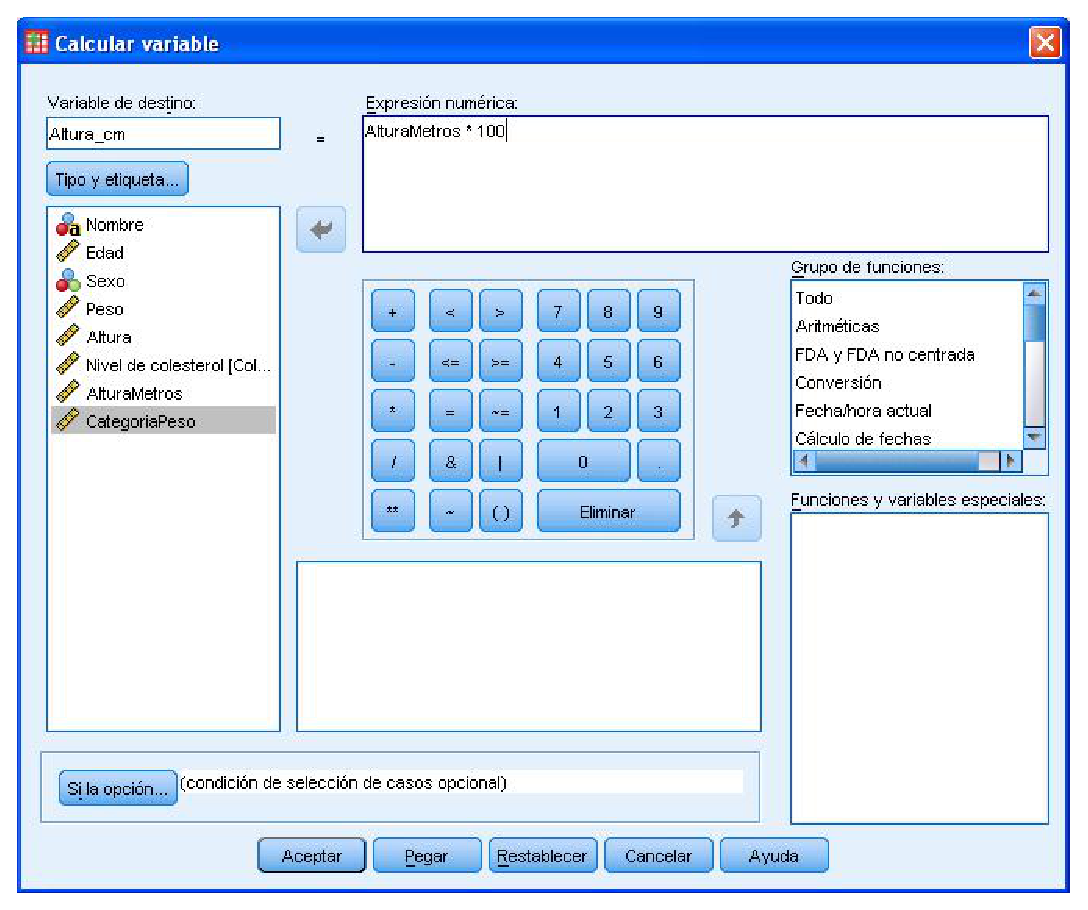
\includegraphics[scale=0.6]{introduccion_spss/img/transformacion}
\caption{Ventana de transformación de variables. A la izquierda aparecen las variables ya definidas, a la derecha las funciones predefinidas que pueden utilizarse, y en el centro los operadores aritméticos y relacionales más comunes.}
\label{g:transformacion}
\end{center}
\end{figure}

En esta ventana se debe introducir el nombre de la nueva variable en el cuadro \opcion{Variable de destino}, y la expresión cuyo resultado será el contenido de la nueva variable en el cuadro \opcion{Expresión numérica}. Para ello aparecen toda una serie de operadores y funciones para realizar la transformación, así como la lista de variables ya definidas que pueden utilizarse como argumentos de las distintas funciones de transformación.

Los operadores más habituales para construir expresiones son los aritméticos \texttt{+}, \texttt{-}, \texttt{*}, \texttt{/}, \texttt{**} (potenciación), los relacionales \texttt{=}, \texttt{<}, \texttt{>}, \verb"~=", \texttt{<=}, \texttt{>=} y los lógicos \texttt{\&} (Y), \texttt{|} (O) y \verb"~" (negación). Y algunas de las funciones más habituales son: \texttt{ABS} (valor absoluto), \texttt{SQRT} (raíz cuadrada), \texttt{EXP} (exponencial), \texttt{LN} (logaritmo neperiano), \texttt{SIN} (seno), \texttt{COS} (coseno), \texttt{TAN} (tangente), \texttt{SUM} (suma), \texttt{MEAN} (media aritmética), \texttt{SD} (desviación estándar), \texttt{RND} (redondeo al entero más cercano), \texttt{TRUNC} (parte entera de un número). 

Haciendo click en el botón \boton{Si la opción...} se pueden establecer condiciones de aplicación de la transformación. Para establecer una condición debemos activar la opción \opcion{Incluir si el caso satisface la condición} y  después introducir una condición lógica como por ejemplo \texttt{Sexo=1}. De este modo, la transformación sólo se aplicará a los individuos que cumplan dicha condición.

Una vez definida la expresión hay que hacer click sobre el botón \boton{Aceptar} y automáticamente aparecerá en la vista de datos una nueva columna con los datos transformados de la nueva variable. 

\subsection{Recodificación de datos}
Otra forma de transformar una variable es crear otra cuyos valores sean una recodificación de los de la primera, por ejemplo agrupando en intervalos. Esta recodificación podemos hacerla tanto en la misma variable como en variables diferentes. Para ello se selecciona el menú \menu{Transformar\flecha Recodificar en distintas variables}. Automáticamente aparece la ventana de recodificación de variables tal y como se ve en la figura~\ref{g:recodificacion}.

\begin{figure}[h!]
\begin{center}
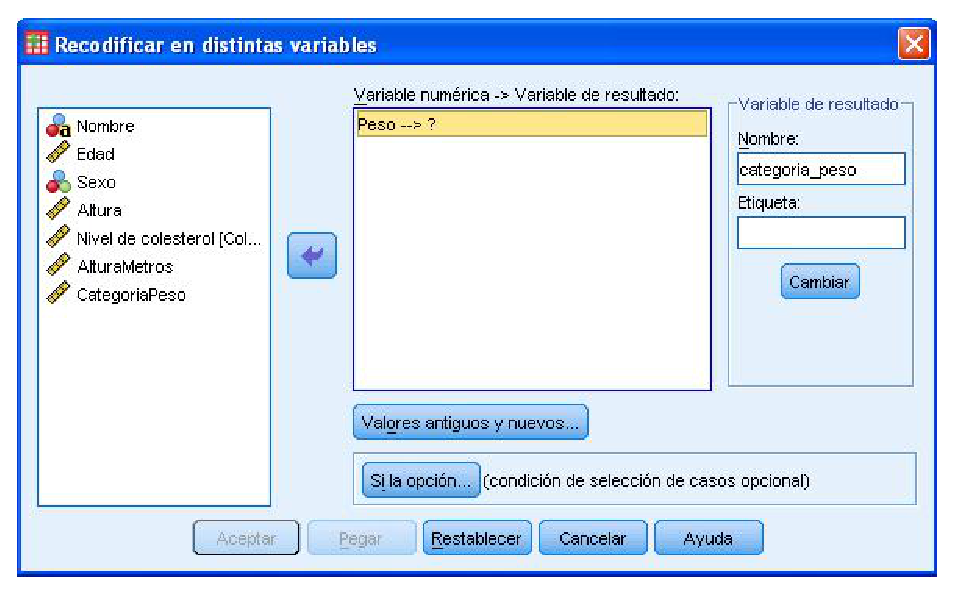
\includegraphics[scale=0.6]{introduccion_spss/img/recodificacion}
\caption{Ventana de recodificación de variables. A la izquierda aparecen las variables ya definidas, a la derecha deben especificarse las reglas de recodificación.}
\label{g:recodificacion}
\end{center}
\end{figure}

Para recodificar una variable en otra nueva, primero debemos seleccionar la variable que queremos recodificar y hacer click sobre el botón con una flecha que aparece al lado. Después hay que escribir el nombre de la nueva variable en el cuadro \opcion{Nombre} y hacer click sobre el botón \boton{Cambiar}. A continuación hay que establecer las reglas de recodificación. Para ello hay que hacer click en el botón \boton{Valores antiguos y nuevos} para que aparezca la ventana de definición de reglas (figura~\ref{g:definicion_intervalos}). Las reglas pueden establecer la conversión del valor de la variable original que introduzcamos en el cuadro \opcion{Valor antiguo} en el valor de la variable nueva que introduzcamos en el cuadro \opcion{Valor nuevo}, o bien la conversión de todo un intervalo de valores de la variable original en un valor de la variable nueva. Una vez definidos dichos valores hay que hacer click sobre el botón \boton{Continuar}, y después sobre \boton{Aceptar}.

\begin{figure}[h!]
\begin{center}
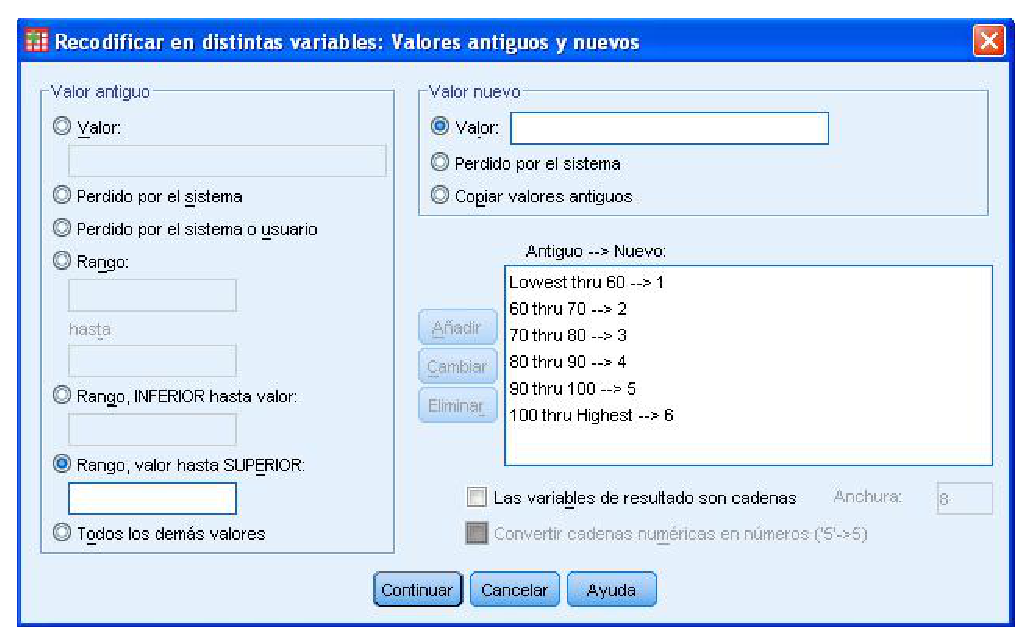
\includegraphics[scale=0.6]{introduccion_spss/img/definicion_intervalos}
\caption{Ventana de definición de reglas.}
\label{g:definicion_intervalos}
\end{center}
\end{figure}

\subsection{Impresión}
Para imprimir se utiliza el menú \menu{Archivo\flecha Imprimir}. Al instante aparece un cuadro de diálogo para la impresión donde debemos indicar si queremos imprimir todo o bien la selección que hayamos hecho. Tras esto se hace click sobre el botón \boton{Aceptar} y la información se envía a la impresora.

Antes de imprimir conviene hacer una previsualización de lo que se va a enviar a la impresora para estar seguros de que es eso lo que se
quiere. Para ello se utiliza el menú \menu{Archivo\flecha Presentación preliminar}. Entonces aparece un visor donde se ve la página, tal y como
se enviará a la impresora. Si todo parece correcto se puede hacer click sobre el botón \boton{Imprimir} y aparecerá el cuadro de diálogo de
impresión desde el que se puede enviar a la impresora definitivamente.

\subsection{Salir del programa}
Para terminar una sesión de trabajo se utiliza el menú \menu{Archivo\flecha Salir}, o bien se hace click sobre el aspa para cerrar la ventana del programa. Si quedan datos o resultados que no se han guardado, el programa nos preguntará antes de salir si deseamos guardarlos.

\subsection{Ayuda}
En esta práctica sólo hemos descrito las operaciones básicas en una sesión de trabajo. Pero quedan por describir todos los análisis estadísticos que pueden realizarse con los menús de la barra de menús. Aunque muchos de estos menús se explicarán en las siguientes prácticas, el programa dispone del menú de ayuda \menu{Ayuda} en el que podemos encontrar una descripción de todos estos menús y al que podemos recurrir cada vez que tengamos dudas.

\clearpage
\newpage

\section{Ejercicios resueltos}
\begin{enumerate}[leftmargin=*]
\item Introducir en la matriz de datos los datos de la siguiente muestra y guardarlos en un fichero con el nombre \texttt{datos\_colesterol.sav}.
\begin{center}
\begin{tabular}{|l|c|r|r|r|}
\hline
\multicolumn{1}{|c|}{Nombre} & \multicolumn{1}{c|}{Sexo} & \multicolumn{1}{c|}{Peso} & \multicolumn{1}{c|}{Altura} & \multicolumn{1}{c|}{Colesterol}\\
\hline
José Luis Martínez Izquierdo  & H &  85 & 179 & 182\\
Rosa Díaz Díaz & M & 65 & 173 & 232\\
Javier García Sánchez  & H & 71 & 181 & 191\\
Carmen López Pinzón & M &  65 & 170 & 200\\
Marisa López Collado & M &  51 & 158 & 148\\
Antonio Ruiz Cruz & H & 66 & 174 & 249\\
Antonio Fernández Ocaña & H &  62 & 172 & 276\\
Pilar Martín González & M &  60 & 166 & 213\\
Pedro Gálvez Tenorio & H &  90 & 194 & 241\\
Santiago Reillo Manzano & H &  75 & 185 & 280\\
Macarena Álvarez Luna & M &  55 & 162 & 262\\
José María de la Guía Sanz & H &  78 & 187 & 198\\
Miguel Angel Cuadrado Gutiérrez & H &  109  & 198 & 210\\
Carolina Rubio Moreno & M &  61 & 177 & 194\\
\hline
\end{tabular}
\end{center}


\begin{indicacion}
\begin{enumerate}
\item En la ventana de \opcion{Vista de variables}, crear las variables \variable{Nombre}, \variable{Sexo},  \variable{Peso}, \variable{Altura} y \variable{Colesterol} e introducir los datos anteriores, siguiendo las indicaciones del apartado~\ref{s:introduccion_datos}.

\item Una vez introducidos los datos, se guardan en un fichero de nombre \texttt{datos colesterol}
siguiendo lo indicado en el apartado~\ref{s:guardar_datos}.
\end{enumerate}
\end{indicacion}


\item Sobre la matriz de datos del ejercicio anterior realizar las siguientes operaciones:

\begin{enumerate}
\item Insertar detrás de la variable \variable{Nombre} una nueva variable \variable{Edad} con las edades
de todos los individuos de la muestra.
\begin{center}
\begin{tabular}{|l|r|}
\hline
\multicolumn{1}{|c|}{Nombre} & \multicolumn{1}{c|}{Edad} \\
\hline
José Luis Martínez Izquierdo & 18 \\
Rosa Díaz Díaz & 32 \\
Javier García Sánchez & 24 \\
Carmen López Pinzón & 35 \\
Marisa López Collado & 46 \\
Antonio Ruiz Cruz & 68 \\
Antonio Fernández Ocaña & 51 \\
Pilar Martín González & 22 \\
Pedro Gálvez Tenorio & 35 \\
Santiago Reillo Manzano & 46 \\
Macarena Álvarez Luna & 53 \\
José María de la Guía Sanz & 58 \\
Miguel Angel Cuadrado Gutiérrez & 27 \\
Carolina Rubio Moreno & 20 \\
\hline
\end{tabular}
\end{center}

\begin{indicacion}
\begin{enumerate}
\item En la \opcion{Vista de variables} seleccionar la fila correspondiente a la variable \variable{Sexo} haciendo click con el ratón sobre
la cabecera de la misma y a continuación seleccionar el menú \menu{Edición\flecha Insertar variable}, con lo que aparece una
nueva fila entre las variables \variable{Nombre} y \variable{Sexo}.
\item En la nueva fila definir la variable \variable{Edad} e introducir los datos anteriores.
\item En la \opcion{Vista de datos} rellenar los datos de la columna correspondiente a la \variable{Edad}.
\end{enumerate}
\end{indicacion}

\item Insertar entre los individuos 4º y 5º los datos correspondientes al siguiente individuo
\begin{quote}
Nombre: Cristóbal Campos Ruiz.\\
Edad: 44 años.\\
Sexo: Hombre.\\
Peso: 70 Kg.\\
Altura: 178 cm.\\
Colesterol: 220 mg/dl.
\end{quote}

\begin{indicacion}
\begin{enumerate}
\item Seleccionar la fila correspondiente al 5º individuo, haciendo click con el ratón sobre la cabecera de la misma y a continuación seleccionar el menú \menu{Edición\flecha Insertar caso}, con lo que aparece una nueva fila entre las correspondientes a los individuos 4º y 5º.
\item Introducir en la nueva fila los datos que se indican.
\end{enumerate}
\end{indicacion}


\item Cambiar el valor de la variable \variable{Peso} de Macarena Álvarez Luna por 58.
\begin{indicacion}
Hacer click con el ratón en la casilla cuyo contenido se desea modificar, escribir $58$ y pulsar \boton{Enter}.
\end{indicacion}

\item Transformar la variable \variable{Altura} para que aparezca expresada en metros.
\begin{indicacion}
\begin{enumerate}
\item Seleccionar el menú~\menu{Transformar\flecha Calcular variable}.
\item En la ventana de transformación de datos introducir el nombre \variable{Altura\_metros} en el cuadro \opcion{Variable de destino}.
\item Introducir la expresión \texttt{Altura/100} en el cuadro \opcion{Expresión numérica}.
\item Hacer click sobre el botón~\boton{Aceptar}. 
\end{enumerate}
\end{indicacion}

\item Recodificar la variable peso en las siguientes cuatro categorias, teniendo en cuenta el sexo:
\begin{center}
  \begin{tabular}{|l|c|c|}  
  \hline
    Categoria & Hombres & Mujeres \\
    \hline
    Bajo      &  $\leq 70$ & $\leq 60$ \\
    Medio     &  (70,85] & (60,70] \\
    Alto      &  (85,100] & (70,80] \\
    Muy Alto  &  $>100$ & $>80$ \\ 
    \hline
  \end{tabular}
\end{center}
\begin{indicacion}
\begin{enumerate}
\item Seleccionar el menú~\menu{Transformar\flecha Recodificar en distintas variables}.
\item En la ventana de recodificación de datos seleccionar la variable \variable{Peso} y hacer click sobre el botón con una flecha que aparece al lado. 
\item Escribir el nombre de la variable recodificada \texttt{Categoria\_Peso} en el cuadro \opcion{Nombre} de la \opcion{Variable de resultado} y hacer click sobre el botón \boton{Cambiar}. 
\item Hacer click en el botón \boton{Valores antiguos y nuevos} para abrir la ventana de definición de reglas de recodificación. 
\item Para definir las reglas de recodificación de los hombres,
\begin{enumerate}[i]
\item Seleccionar la opción \opcion{Rango INFERIOR hasta valor} del cuadro \opcion{Valor antiguo} e introducir 70 en el cuadro
correspondiente. Introducir 1 en el cuadro de la opción \opcion{Valor} del cuadro \opcion{Valor nuevo} y hacer click en el botón
\boton{Añadir}.
\item Seleccionar la opción \opcion{Rango} del cuadro \opcion{Valor antiguo} e introducir 70 en el cuadro correspondiente y 85 en el cuadro
\opcion{hasta}. Introducir 2 en el cuadro de la opción \opcion{Valor} del cuadro \opcion{Valor nuevo} y hacer click en el botón
\boton{Añadir}.
\item Seleccionar la opción \opcion{Rango} del cuadro \opcion{Valor antiguo} e introducir 85 en el cuadro correspondiente y 100 en el cuadro
\opcion{hasta}. Introducir 3 en el cuadro de la opción \opcion{Valor} del cuadro \opcion{Valor nuevo} y hacer click en el botón
\boton{Añadir}.
\item Seleccionar la opción \opcion{Rango valor hasta SUPERIOR} del cuadro \opcion{Valor antiguo} e introducir 100 en el cuadro
correspondiente. Introducir 4 en el cuadro de la opción \opcion{Valor} del cuadro \opcion{Valor nuevo} y hacer click en el botón
\boton{Añadir}.
\end{enumerate}
\item Hacer click en el botón \boton{Continuar} para cerrar la ventana. 
\item Hacer click en el botón \boton{Si la opción...} para abrir la ventana de definición de concidiones.
\item Seleccionar la opción \opcion{Incluir si el caso satisface la condición} e introducir la condición \texttt{Sexo=``H''} en el cuadro
correspondiente.
\item Hacer click en el botón \boton{Continuar} para cerrar la ventana.
\item Hacer click en el botón \boton{Aceptar}.
\item Repetir los mismos pasos para establecer las reglas de codificación de las mujeres.
\item En \menu{Vista de variables} hacer clik en \boton{Valores de Categoria\_Peso}, y en \opcion{Etiquetas de valor} ir asignando a los
valores $1$, $2$, $3$ y $4$ las etiquetas \texttt{Bajo}, \texttt{Medio}, \texttt{Alto} y \texttt{Muy alto} respectivamente, haciendo click
en el botón \boton{Añadir} después de cada asignación, y una vez terminado hacer click en el \boton{Aceptar}.
\end{enumerate}
\end{indicacion}

\item Volver a guardar los cambios en el fichero anterior y salir del programa.
\begin{indicacion}
\begin{enumerate}
\item Seleccionar el menú \menu{Archivo\flecha Guardar}.
\item Seleccionar el menú \menu{Archivo\flecha Salir}.
\end{enumerate}
\end{indicacion}

\end{enumerate}
\end{enumerate}

%\section{Caso práctico}
%Se ha diseñado un ensayo clínico aleatorizado, doble-ciego y
%controlado con placebo, para estudiar el efecto de dos
%alternativas terapéuticas en el control de la hipertensión
%arterial. Se han reclutado 100 pacientes hipertensos y estos han
%sido distribuidos aleatoriamente en tres grupos de tratamiento. A
%uno de los grupos (control) se le administró un placebo, a otro
%grupo se le administró un inhibidor de la enzima conversora de la
%angiotensina (IECA) y al otro un tratamiento combinado de un
%diurético y un Antagonista del Calcio. Las variables respuesta
%final fueron las presiones arteriales sistólica y diastólica.
%
%
%Los datos con las claves de aleatorización han sido introducidos
%en una base de datos que reside en la central de aleatorización,
%mientras que los datos clínicos han sido archivados en dos
%archivos distintos, uno para cada uno de los dos centros
%participantes en el estudio.
%
%Las variables almacenadas en estos archivos clínicos son las
%siguientes:
%
%\begin{itemize}
%\item CLAVE Clave de aleatorización
%\item NOMBRE  Iniciales del paciente
%\item F\_NACIM  Fecha de Nacimiento
%\item F\_INCLUS Fecha de inclusión
%\item SEXO  Sexo (0: Hombre 1: Mujer)
%\item ALTURA Altura en cm.
%\item PESO  Peso en Kg.
%\item PAD\_INI  Presión diastólica basal (inicial)
%\item PAD\_FIN  Presión diastólica final
%\item PAS\_INI Presión sistólica basal (inicial)
%\item PAS\_FIN  Presión sistólica final
%\end{itemize}
%
%El archivo de claves de aleatorización contiene sólo dos
%variables.
%
%\begin{itemize}
%    \item CLAVE Clave de aleatorización
%    \item FARMACO Fármaco administrado (0: Placebo, 1: IECA,  2:Ca Antagonista + diurético)
%\end{itemize}
%
%Se pide:
%
%\begin{enumerate}
%\item Leer los datos del centro con 10 pacientes, incluidos en el
%archivo \textsf{Hipertensos HA.xls}, este hospital trabaja con la
%hoja de cálculo Excel.
%
%\begin{indicacion}
%Desplegar el menú \menu{Archivo\flecha Abrir\flecha Datos}, e ir hasta el
%directorio que contiene el archivo \textsf{Hipertensos HA.xls},
%escogiendo como tipo de archivo el formato de Excel. Una vez tenemos
%delante el nombre del archivo, para abrirlo será suficiente con un
%doble clik, pero teniendo en cuenta que hay que activar la opción
%\opcion{Leer nombres de variables} si queremos que utilice la primera
%fila del archivo de Excel para dar nombre a las variables en el
%archivo de datos de SPSS.
%\end{indicacion}
%
%\item Añadir a estos, los datos de los pacientes 11 al 100,
%incluidos en el archivo \textsf{Hipertensos HB} y guardar los datos
%como \textsf{Hipertensos totales}.
%
%
%\begin{indicacion}
%\begin{enumerate}
%\item Teniendo en cuenta que lo que pretendemos es añadir nuevos casos
%a un archivo de datos ya abierto, el menú a utilizar es
%\menu{Datos\flecha Fundir archivos\flecha Añadir casos}. Después activamos la
%opción \opcion{Un archivo de datos de SPSS Statistics externo}, y con el botón
%\boton{Examinar} accedemos hasta la carpeta que contenga el archivo
%\textsf{Hipertensos HB}. Una vez seleccionado, utilizamos el botón
%\boton{Continuar}, y posteriormente el botón \boton{Aceptar} en el
%siguiente cuadro de diálogo que aparece.
%\item Una vez generado el archivo de datos, para guardarlo podemos
%utilizar el menú \menu{Archivo\flecha Guardar como}.
%\end{enumerate}
%\end{indicacion}
%
%\item Fusionar los datos clínicos con las claves de
%aleatorización. El fichero con las claves se denomina
%\textsf{Claves aleatorizacion}. Grabar el archivo resultante con
%el nombre \textsf{Hipertensos Datos Claves}
%
%\begin{indicacion}
%De forma similar al apartado anterior pero teniendo en cuenta que
%ahora lo que pretendemos es añadir variables. Para ello utilizamos el menú:
%\menu{Datos\flecha Fundir archivos\flecha Añadir variables}, para acceder
%después hasta el archivo \textsf{Claves aleatorizacion}, y
%posteriormente vamos aceptando en todos los cuadros de diálogo que
%aparecen. Una vez generado, guardamos el nuevo archivo de datos y
%claves: menú \menu{Archivo\flecha Guardar como}.
%\end{indicacion}
%
%\item Crear un archivo para cada uno de los grupos de tratamiento.
%Denominar a estos archivos \textsf{Hipertensos placebo},
%\textsf{Hipertensos IECA} e \textsf{Hipertensos Ca}
%respectivamente.
%
%\begin{indicacion}
%Se podría lograr el mismo resultado de múltiples maneras. Por
%ejemplo:
%\begin{enumerate}
%\item Segmentando el archivo mediante el menú \menu{Datos\flecha Dividir archivo...}, y \opcion{Organizar los resultados por grupos} basados en
%la variable \variable{farmaco}. Una vez dividido el archivo,
%podemos marcar los casos correspondientes a cada uno de los fármacos
%y hacer un cortar y pegar en un nuevo archivo específico para cada
%fármaco.
%\item También podemos generar los nuevos archivos utilizando el
%sistema de filtros de SPSS. Para ello el menú a utilizar es
%\menu{Datos\flecha Seleccionar Casos...}, con la opción \opcion{Si se
%satisface la condición}, botón \boton{Si la op...}, y entramos en un cuadro
%de diálogo en el que damos forma a la condición, que en primera
%instancia será \variable{farmaco=0}, para volver al cuadro de
%diálogo anterior y escoger la opción \opcion{Copiar casos seleccionados 
%a un nuevo conjunto de datos} y poner en \opcion{Nombre de 
%conjunto de datos:} \textsf{Hipertensos\_placebo}. Igualmente, 
%repetiríamos el proceso para los otros dos fármacos.
%\end{enumerate}
%\end{indicacion}
%
%\item Calcular, para cada paciente, la edad en años el día de la
%incorporación al estudio (redondeando al entero más próximo).
%Denominar la nueva variable \variable{edad} y etiquetarla
%correspondientemente.
%
%\begin{indicacion}
%Internamente SPSS trabaja con las variables en formato fecha
%almacenando el número de segundos transcurridos desde el comienzo
%del Calendario Gregoriano en el año 1582 hasta la fecha que
%introducimos. Por lo tanto, si restamos dos variables en formato
%fecha, no nos da el número de años transcurridos entre una y otra,
%sino el número de segundos. Por ello, la nueva variable obtenida
%como resultado de la resta hay que dividirla entre el número de
%segundos que tiene un año a razón de 3600 segundos la hora, 24 horas
%el día, y $365.25$ días el año, aproximadamente. Teniendo en cuenta
%lo anterior, el proceso a utilizar es: Menú
%\menu{Transformar\flecha Calcular variable}, y en \opcion{Variable de
%destino}, escribimos \variable{edad}. Como
%expresión numérica para su cálculo introducimos:
%
%\begin{center}
%\comando{(F\_INCLUS - F\_NACIM)/(365.25 * 24 * 3600)}
%\end{center}
%\end{indicacion}
%
%\item Recodificar dicha edad de forma que la nueva variable, de
%nombre \variable{grupoedad}, tome los siguientes valores y etiquetas
%de valor:
%
%\begin{center}
%
%\begin{tabular}{|l|l|l|}
%\hline
%\multicolumn{1}{|c|}{Edad en años} & \multicolumn{1}{c|}{Grupo edad} & \multicolumn{1}{c|}{Etiqueta} \\
%\hline
%\multicolumn{1}{|c|}{Edad $\leq 37$} & \multicolumn{1}{c|}{1} & \multicolumn{1}{c|}{Hasta 37 inclusive} \\
%\hline
%\multicolumn{1}{|c|}{$37<$ Edad $\leq 44$} & \multicolumn{1}{c|}{2} & \multicolumn{1}{c|}{De 37 a 44} \\
%\hline
%\multicolumn{1}{|c|}{$44<$ Edad $\leq 51$} & \multicolumn{1}{c|}{3} & \multicolumn{1}{c|}{De 44 a 51} \\
%\hline
%\multicolumn{1}{|c|}{Edad $>51$} & \multicolumn{1}{c|}{4} & \multicolumn{1}{c|}{Mayores de 51} \\
%\hline
%\end{tabular}
%
%\end{center}
%
%\begin{indicacion}
%Para recodificar una variable, se utiliza el proceso ya explicado en
%la práctica de Introducción a SPSS, con el menú
%\menu{Transformar\flecha Recodificar en distintas variables}, 
%escogiendo \variable{edad}
%como \opcion{Variable de entrada}, y dando el nombre 
%\variable{grupoedad} a la \opcion{Variable
%de resultado}, utilizando el botón \boton{Cambiar}, y posteriormente
%el botón \boton{Valores antiguos y nuevos} para delimitar las
%categorías de la nueva variable.
%\end{indicacion}
%
%
%
%
%\item Calcular, para cada paciente, el índice de masa corporal (se
%obtiene dividiendo el peso, expresado en kg, entre la altura,
%expresada en m, elevada al cuadrado) y almacenar el resultado en la
%variable \variable{masacorp}.
%
%\begin{indicacion}
%Con el menú \menu{Transformar\flecha Calcular variable}, escogiendo como
%variable de destino \variable{masacorp}, y como expresión numérica
%la indicada en el enunciado.
%\end{indicacion}
%
%\item Recodificar dicho índice de masa corporal, de forma que la
%nueva variable, de nombre \variable{obesidad}, tome los siguientes
%valores y etiquetas de valor según el sexo del paciente.
%
%\begin{center}
%\begin{tabular}{|l|l|l|l|}
%\hline
%\multicolumn{1}{|c|}{Sexo} & \multicolumn{1}{c|}{Masacorp} & \multicolumn{1}{c|}{Obesidad} & \multicolumn{1}{c|}{Etiqueta} \\
%\hline
%\multicolumn{1}{|c|}{} & \multicolumn{1}{c|}{$\leq 21$} & \multicolumn{1}{c|}{1} & \multicolumn{1}{c|}{Desnutrido} \\
%\cline{2-4}
%\multicolumn{1}{|c|}{} & \multicolumn{1}{c|}{$(21,\,26.94]$} & \multicolumn{1}{c|}{2} & \multicolumn{1}{c|}{Normal} \\
%\cline{2-4}
%\multicolumn{1}{|c|}{0} & \multicolumn{1}{c|}{$(26.94,\, 32.94]$} & \multicolumn{1}{c|}{3} & \multicolumn{1}{c|}{Sobrepeso} \\
%\cline{2-4}
%\multicolumn{1}{|c|}{} & \multicolumn{1}{c|}{$(32.94,\, 43.94]$} & \multicolumn{1}{c|}{4} & \multicolumn{1}{c|}{Obeso} \\
%\cline{2-4}
%\multicolumn{1}{|c|}{} & \multicolumn{1}{c|}{$>43.94$} & \multicolumn{1}{c|}{5} & \multicolumn{1}{c|}{Muy obeso} \\
%\hline
%\multicolumn{1}{|c|}{} & \multicolumn{1}{c|}{$\leq 19$} & \multicolumn{1}{c|}{1} & \multicolumn{1}{c|}{Desnutrido} \\
%\cline{2-4}
%\multicolumn{1}{|c|}{} & \multicolumn{1}{c|}{$(19,\, 24.94]$} & \multicolumn{1}{c|}{2} & \multicolumn{1}{c|}{Normal} \\
%\cline{2-4}
%\multicolumn{1}{|c|}{1} & \multicolumn{1}{c|}{$(24.94,\,29.94]$} & \multicolumn{1}{c|}{3} & \multicolumn{1}{c|}{Sobrepeso} \\
%\cline{2-4}
%\multicolumn{1}{|c|}{} & \multicolumn{1}{c|}{$(29.94,\,39.94]$} & \multicolumn{1}{c|}{4} & \multicolumn{1}{c|}{Obeso} \\
%\cline{2-4}
%\multicolumn{1}{|c|}{} & \multicolumn{1}{c|}{$>39,94$} & \multicolumn{1}{c|}{5} & \multicolumn{1}{c|}{Muy obeso} \\
%\hline
%\end{tabular}
%
%\begin{indicacion} 
%Se trata de un problema de recodificación, muy parecido al explicado en la indicación del punto 6, con la única novedad
%de que ahora hay que hacer una doble recodificación: por un lado para hombres y por el otro para mujeres. Para ello, después de escoger las
%variables de entrada y de resultado, haciendo uso del botón condicional \boton{Si la opción} podemos escoger únicamente los casos que
%cumplen la condición impuesta por la variable \variable{Sexo}; es decir, con la condición \variable{Sexo=0}, recodificamos en primera
%instancia el índice de masa corporal de los hombres, y con \variable{Sexo=1} recodificamos el de las mujeres.
%\end{indicacion}
%
%\end{center}
%
%\end{enumerate}

% Version control information:
%$HeadURL: https://practicas-spss.googlecode.com/svn/trunk/distribuciones_graficas/distribuciones_graficas.tex $
%$LastChangedDate: 2010-09-27 16:37:11 +0200 (lun, 27 sep 2010) $
%$LastChangedRevision: 3 $
%$LastChangedBy: asalber $
%$Id: distribuciones_graficas.tex 3 2010-09-27 14:37:11Z asalber $

\chapter[Distribuciones de Frecuencias y Representaciones Gráficas]{Distribuciones de Frecuencias \\ y Representaciones Gráficas}

\section{Fundamentos teóricos}
Uno de los primeros pasos en cualquier estudio estadístico es el resumen y la descripción de la información contenida en una muestra.
Para ello se van a aplicar algunos métodos de análisis descriptivo, que nos permitirán clasificar y estructurar la información al igual que representarla gráficamente.

Las características que estudiamos pueden ser o no susceptibles de medida; en este sentido definiremos una \emph{variable} como un carácter susceptible de ser medido, es decir, cuantitativo y cuantificable mediante la observación, (por ejemplo el peso de las personas, la edad, etc...), y definiremos un \emph{atributo} como un carácter no susceptible de ser medido, y en consecuencia observable tan sólo cualitativamente (por ejemplo el color de ojos, estado de un paciente, etc...).
Se llaman modalidades a las posibles observaciones de un atributo.

Dentro de los atributos, podemos hablar de \emph{atributos ordinales}, los que presentan algún tipo de orden entre las distintas modalidades, y de \emph{atributos nominales}, en los que no existe ningún orden entre ellas.

Dentro de las variables podemos diferenciar entre \emph{discretas}, si sus valores posibles son valores aislados, y \emph{continuas}, si pueden tomar cualquier valor dentro de un intervalo.

En algunos textos no se emplea el término \emph{atributo} y se denominan a todos los caracteres \emph{variables}. En ese caso se distinguen \emph{variables cuantitativas} para designar las que aquí hemos definido como \emph{variables}, y \emph{variables cualitativas} para las que aquí se han llamado \emph{atributos}.
En lo sucesivo se aplicará este criterio para simplificar la exposición.

\subsection{Cálculo de frecuencias}

Para estudiar cualquier característica, lo primero que deberemos hacer es un recuento de las observaciones, y el número de repeticiones de éstas. Para cada valor $x_i$ de la muestra se define:
\begin{description}
\item[Frecuencia absoluta] Es el número de veces que aparece cada uno de los valores $x_i$ y se denota por $n_i$.

\item [Frecuencia relativa] Es el número de veces que aparece cada valor $x_i$ dividido entre el tamaño muestral y se denota por $f_i$

\[f_i=\frac{n_i}{n}\]

Generalmente las frecuencias relativas se multiplican por $100$ para que representen el tanto por ciento.
\end{description}

En el caso de que exista un orden entre los valores de la variable, a veces nos interesa no sólo conocer el número de veces que se repite un determinado valor, sino también el número de veces que aparece dicho valor y todos los anteriores.
A este tipo de frecuencias se le denomina \emph{frecuencias acumuladas}.

\begin{description}
\item [Frecuencia absoluta acumulada] Es la suma de las frecuencias absolutas de los valores menores que $x_i$ más la frecuencia absoluta de $x_i$, y se denota por $N_i$

\[N_i=n_1+n_2+\ldots+n_i\]

\item [Frecuencia relativa acumulada] Es la suma de las frecuencias relativas de los valores menores que $x_i$ más la frecuencia relativa de $x_i$, y se denota por $F_i$

\[F_i=f_1+f_2+\ldots+f_i\]
\end{description}

Los resultados de las observaciones de los valores de una variable estadística en una muestra suelen representarse en forma de tabla.
En la primera columna se representan los valores $x_i$ de la variable colocados en orden creciente, y en la siguiente columna los valores de las frecuencias absolutas correspondientes $n_i$.

Podemos completar la tabla con otras columnas, correspondientes a las frecuencias relativas, $f_i$, y a las frecuencias acumuladas, $N_i$ y $F_i$.
Al conjunto de los valores de la variable observados en la muestra junto con sus frecuencias se le conoce como \emph{distribución de frecuencias muestral}.

\begin{ejemplo}
En una encuesta a 25 matrimonios, sobre el número de hijos que tienen, se obtienen los siguientes datos:

1, 2, 4, 2, 2, 2, 3, 2, 1, 1, 0, 2, 2, 0, 2, 2, 1, 2, 2, 3, 1, 2,
2, 1, 2.

Los valores distintos de la variable son: 0, 1, 2, 3 y 4. Así frecuencia absoluta sería:
\[
\begin{array}{|c|l|r|}
\hline
x_i & Recuento & n_i \\ \hline
0 & II & 2 \\
1 & IIIII I & 6 \\
2 & IIIII IIIII IIII & 14 \\
3 & II & 2 \\
4 & I & 1 \\ \hline
\end{array}
\]

Y la tabla de distribución de las frecuencias sería:
\[
\begin{array}{|c|c|c|c|c|}
\hline
x_i & n_i & f_i & N_i & F_i \\ \hline
0 & 2 & 0.08 & 2 & 0.08 \\ \hline
1 & 6 & 0.24 & 8 & 0.32 \\ \hline
2 & 14 & 0.56 & 22 & 0.88 \\ \hline
3 & 2 & 0.08 & 24 & 0.96 \\ \hline
4 & 1 & 0.04 & 25 & 1 \\ \hline
\mbox{Suma} & 25 & 1 & \multicolumn{2}{c}{} \\
\cline{1-3}
\end{array}
\]

\end{ejemplo}

Cuando el tamaño de la muestra es grande en el caso de variables discretas con muchos valores distintos de la variable, y en cualquier caso si se trata de variables continuas, se agrupan las observaciones en \emph{clases}, que son intervalos contiguos, preferiblemente de la misma amplitud.

Para decidir el número de clases a considerar, una regla frecuentemente utilizada es tomar el entero más próximo a $\sqrt{n}$ donde $n$ es el número de observaciones en la muestra.
Pero conviene probar con distintos números de clases y escoger el que proporcione una descripción más clara.
Así se prefijan los intervalos $(a_{i-1},a_i] , i=1,2,\ldots,l$ siendo $a=a_0<a_1<....<a_l=b$ de tal modo que todos los valores observados estén dentro del intervalo $(a, b]$, y sin que exista ambig\"{u}edad a la hora de decidir a qué intervalo pertenece cada dato.

Llamaremos \emph{marca de clase} al punto medio de cada intervalo. 
Así la \emph{marca de la clase} $(a_{i-1},a_i]$ es el punto medio
$x_i$ de dicha clase, es decir
\[ x_i=\frac{a_{i-1}+a_i}{2} \]

En el tratamiento estadístico de los datos agrupados, todos los valores que están en una misma clase se consideran
iguales a la marca de la clase.
De esta manera si en la clase $(a_{i-1},a_i]$ hay $n_i$ valores observados, se puede asociar la marca de la clase $x_i$ con esta frecuencia $n_i$.


\subsection{Representaciones gráficas}

Hemos visto que la tabla estadística resume los datos de una muestra, de forma que ésta se puede analizar de una manera más sistemática y resumida.
Para conseguir una percepción visual de las características de la población resulta muy útil el uso de gráficas y diagramas. Dependiendo del tipo de variable y de si trabajamos con datos agrupados o no, se utilizarán distintos tipos.


\subsubsection{Diagrama de barras y polígono de frecuencias}

Consiste en representar sobre el eje de abscisas de un sistema de ejes coordenados los distintos valores de la variable $X$, y levantar sobre cada uno de esos puntos una barra cuya altura sea igual a la frecuencia absoluta o relativa correspondiente a ese valor, tal y como se muestra en la figura \ref{g:diagramaabsolutas}.
Esta representación se utiliza para distribuciones de frecuencias con pocos valores distintos de la variable, tanto cuantitativas como cualitativas, y en este ultimo caso se suele representar con rectángulos de altura igual a la frecuencia de cada modalidad.

En el caso de variables cuantitativas se puede representar también el diagrama de barras de las frecuencias acumuladas, tal y como se muestra en la figura \ref{g:diagramaacumuladas}.

Otra representación habitual es el \emph{polígono de frecuencias} que consiste en la línea poligonal cuyos vertices son los puntos $(x_i,n_i)$, tal y como se ve en la figura \ref{g:poligonoabsolutas}, y si en vez de considerar las frecuencias absolutas o relativas se consideran las absolutas o relativas acumuladas, se obtiene el \emph{polígono de frecuencias acumuladas}, como se ve en la figura \ref{g:poligonoacumuladas}.

\begin{figure}[h!]
\centering
\subfigure[Diagrama de barras de frecuencias absolutas.]{\label{g:diagramaabsolutas}
\scalebox{0.65}{\input{distribuciones_graficas/img/diagrama_barras_frecuencia_absoluta}}}\qquad
\subfigure[Diagrama de barras de frecuencias absolutas acumuladas.]{\label{g:diagramaacumuladas}
\scalebox{0.65}{\input{distribuciones_graficas/img/diagrama_barras_frecuencia_acumulada}}}\\
\subfigure[Polígono de frecuencias absolutas.]{\label{g:poligonoabsolutas}
\scalebox{0.65}{\input{distribuciones_graficas/img/poligono_frecuencia_absoluta}}}\qquad
\subfigure[Polígono de frecuencias absolutas acumuladas]{\label{g:poligonoacumuladas}
\scalebox{0.65}{\input{distribuciones_graficas/img/poligono_frecuencia_acumulada}}}
\caption{Diagramas de barras y polígonos asociados para datos no
agrupados.}
\end{figure}


\subsubsection{Histogramas}

Este tipo de representaciones se utiliza en variables continuas y en variables discretas en que se ha realizado una agrupación de las observaciones en clases. Un \emph{histograma} es un conjunto de rectángulos, cuyas bases son los intervalos de clase $(a_{i-1},a_i]$ sobre el eje $OX$ y su altura la correspondiente frecuencia absoluta
, relativa, absoluta acumulada, o relativa acumulada, tal y como se muestra en la figuras~\ref{g:histogramaabsolutas} y \ref{g:histogramaacumuladas}.
 
Si unimos los puntos medios de las bases superiores de los rectángulos del histograma, se obtiene el \emph{polígono de frecuencias} correspondiente a datos agrupados (figura~\ref{g:poligonoabsolutasagrupado}).

El polígono de frecuencias también se puede utilizar para representar las frecuencias acumuladas, tanto absolutas como relativas.
En este caso la línea poligonal se traza uniendo los extremos derechos de las bases superiores de los rectángulos del histograma de frecuencias acumuladas, en lugar de los puntos centrales (figura~\ref{g:poligonoacumuladasagrupado}).

\begin{figure}[h!]
\centering
\subfigure[Histograma de frecuencias absolutas.]{\label{g:histogramaabsolutas}
\scalebox{0.65}{\input{distribuciones_graficas/img/histograma_frecuencia_absoluta}}}\qquad
\subfigure[Histograma de frecuencias absolutas acumuladas.]{\label{g:histogramaacumuladas}
\scalebox{0.65}{\input{distribuciones_graficas/img/histograma_frecuencia_acumulada}}}\\
\subfigure[Polígono de frecuencias absolutas.]{\label{g:poligonoabsolutasagrupado}
\scalebox{0.65}{\input{distribuciones_graficas/img/poligono_frecuencia_absoluta_agrupado}}}\qquad
\subfigure[Polígono de frecuencias absolutas acumuladas]{\label{g:poligonoacumuladasagrupado}
\scalebox{0.65}{\input{distribuciones_graficas/img/poligono_frecuencia_acumulada_agrupado}}}
\caption{Histograma y polígonos asociados para datos agrupados.}
\end{figure}

Para variables cualitativas y cuantitativas discretas también se pueden usar las superficies representativas; de éstas, las más empleadas son los \emph{sectores circulares}.


\subsubsection{Sectores circulares o diagrama de sectores}

Es una representación en la que un círculo se divide en sectores, de forma que los ángulos, y por tanto las áreas respectivas, sean proporcionales a la frecuencia.

\begin{ejemplo}
Se está haciendo un estudio en una población el grupo sanguíneo de sus ciudadanos. Para ello disponemos de una muestra de 30 personas, con los siguientes resultados: 5 personas con grupo 0, 14 con grupo A, 8 con grupo B y  3 con grupo AB.

El diagrama de sectores de frecuencias relativas correspondiente aparece en la figura~\ref{g:diagramasectoresgruposanguineo}.

\begin{figure}[h!]
\centering
\scalebox{0.7}{\input{distribuciones_graficas/img/diagrama_sectores_grupo_sanguineo}}
\caption{Diagrama de sectores de frecuencias relativas del grupo sanguineo.}
\label{g:diagramasectoresgruposanguineo}
\end{figure}
\end{ejemplo}


\subsubsection{Diagrama de cajas y datos atípicos}
Los datos extremadamente altos o bajos, en comparación con los del resto de la muestra, reciben el nombre de datos influyentes o \emph{datos atípicos}.
Tales datos que, como su propio nombre indica, pueden modificar las conclusiones de un estudio, deben ser considerados atentamente antes de aceptarlos, pues no pocas veces podrán ser, simplemente, datos erróneos. La representación gráfica más apropiada para detectar estos datos es el \emph{diagrama de cajas}.
Este diagrama está formado por una caja que contiene el 50\% de los datos centrales de la distribución, y unos segmentos que salen de la caja, que indican los límites a partir de los cuales los
datos se consideran atípicos.
En la figura~\ref{g:cajas} se puede observar un ejemplo en el que aparecen dos datos atípicos.

\begin{figure}[h!]
\begin{center}
\scalebox{0.8}{\input{distribuciones_graficas/img/diagrama_caja}}
\caption{Diagrama de cajas para una muestra de recién nacidos. Existen dos niños con pesos atípicos, uno con peso extremadamente bajo $1.9$ kg, y otro con peso extremadamente alto $4.5$ kg.}
\label{g:cajas}
\end{center}
\end{figure}

\clearpage
\newpage

\section{Ejercicios resueltos}

\begin{enumerate}[leftmargin=*]
\item  Se realizó una encuesta a 40 personas de más de 70 años sobre el número de medicamentos distintos que tomaban habitualmente. El resultado de dicha encuesta fue el siguiente:
\begin{eqnarray*}
&&3-1-2-2-0-1-4-2-3-5-1-3-2-3-1-4-2-4-3-2 \\
&&3-5-0-1-2-0-2-3-0-1-1-5-3-4-2-3-0-1-2-3
\end{eqnarray*}
Se pide:

\begin{enumerate}
\item  Crear la variable \variable{medicamentos} e introducir los datos.

\item  Construir la tabla de frecuencias.
\begin{indicacion}
\begin{enumerate}
\item Seleccionar el menú \menu{Analizar\flecha Estadísticos descriptivos\flecha Frecuencias}. 
\item Seleccionar la variable \variable{medicamentos} en el campo \opcion{Variables} del cuadro de diálogo. 
\item Activar la opción \opcion{Mostrar tabla de frecuencias} y hacer click en el botón \boton{Aceptar}.
\end{enumerate}
\end{indicacion}

\item  Dibujar el diagrama de barras de las frecuencias absolutas.
\begin{indicacion}
\begin{enumerate}
\item Seleccionar el menú \menu{Gráficos\flecha Cuadros de diálogo antiguos\flecha Barras\flecha Definir}. 
\item Seleccionar la variable \variable{medicamentos} en el campo \opcion{Eje de categorías} del cuadro de diálogo y seleccionar la opción \opcion{Nº de casos}.
\end{enumerate}
\end{indicacion}

\item  Dibujar el polígono de frecuencias absolutas.
\begin{indicacion}
\begin{enumerate}
\item Seleccionar el menú \menu{Gráficos\flecha Cuadros de diálogo antiguos\flecha Líneas\flecha Definir}. 
\item Seleccionar la variable \variable{medicamentos} en el campo \opcion{Eje de categorías} del cuadro de diálogo
 y seleccionar la opción \opcion{Nº de casos}.
\end{enumerate}
\end{indicacion}

\item  Dibujar el diagrama de barras de las frecuencias relativas acumuladas.
\begin{indicacion}
Repetir los mismos pasos del apartado c) pero seleccionando esta vez la opción \opcion{\% acum}.
\end{indicacion}

\item  Dibujar el diagrama de sectores.
\begin{indicacion}
\begin{enumerate}
\item Seleccionar el menú \menu{Gráficos\flecha Cuadros de diálogo antiguos\flecha Sectores\flecha Definir}.
\item Seleccionar la variable \variable{medicamentos} en el campo \campo{Definir sectores por} del cuadro de diálogo.
\end{enumerate}
\end{indicacion}
\end{enumerate}

\item  En un hospital se realizó un estudio sobre el número de personas que ingresaron en urgencias en el mes de
noviembre. Los datos observados fueron:
\begin{eqnarray*}
&&15-23-12-10-28-7-12-17-20-21-18-13-11-12-26 \\
&&29-6-16-39-22-14-17-21-28-9-16-13-11-16-20
\end{eqnarray*}
Se pide:

\begin{enumerate}
\item  Crear la variable \variable{urgencias} e introducir los datos.

\item  Dibujar el histograma de las frecuencias absolutas agrupando en 5 clases desde el 0 hasta el 40.
\begin{indicacion}
\begin{enumerate}
\item Seleccionar el menú \menu{Gráficos\flecha Cuadros de diálogo antiguos\flecha Histograma}.
\item Seleccionar la variable \variable{urgencias} en el campo \campo{Variable} del cuadro de diálogo y hacer click en el botón
\boton{Aceptar}.
\item Editar el histograma haciendo doble click sobre él.
\item En el editor de gráficos hacer click con el botón derecho del ratón 
en la zona del histograma, el cual quedará rodeado de una línea amarilla 
y hacer click en la ventana emergente sobre \opcion{Ventana Propiedades}.  
\item Seleccionar la opción \opcion{Clases de punto}, en \opcion{Eje X} elegir \opcion{Personalizado} y en \opcion{Número de Intervalos}
poner 5. 
\item Hacer click sobre el botón \boton{Aplicar}, después sobre el botón \boton{Cerrar} de la ventana de propiedades y cerrar el editor de
gráficos.
\end{enumerate}
\end{indicacion}

\item  Dibujar el diagrama de cajas. ¿Existe algún dato atípico?
\begin{indicacion}
\begin{enumerate}
\item Seleccionar el menú \menu{Gráficos\flecha Cuadros de diálogo antiguos\flecha 
Diagramas de caja}.
\item Seleccionar la opción \opcion{Resúmenes para distintas variables} y hacer click en el botón \boton{Definir}.
\item Seleccionar la variable \variable{urgencias} en el campo \opcion{Las cajas representan} del cuadro de diálogo y hacer click sobre el botón \boton{Aceptar}.
\end{enumerate}
\end{indicacion}

\item  En el caso de que exista algún dato atípico, eliminarlo y dibujar el histograma de frecuencias absolutas, de forma que aparezcan clases de amplitud 5, comenzando en el 5 y terminando en el 30.
\begin{indicacion}
\begin{enumerate}
\item Identificar el caso que corresponde al dato atípico y eliminarlo en el editor de datos. 
\item Repetir los pasos del apartado b) para dibujar el histograma.
\end{enumerate}
\end{indicacion}
\end{enumerate}

\end{enumerate}


\section{Ejercicios propuestos}
\begin{enumerate}[leftmargin=*]
\item  El número de lesiones padecidas durante una temporada por cada jugador de un equipo de fútbol fue el siguiente:
\begin{center}
0 -- 1 -- 2 -- 1 -- 3 -- 0 -- 1 -- 0 -- 1 -- 2 -- 0 -- 1 \\
1 -- 1 -- 2 -- 0 -- 1 -- 3 -- 2 -- 1 -- 2 -- 1 -- 0 -- 1
\end{center}

Se pide:
\begin{enumerate}
\item Crear la variable lesiones e introducir los datos.
\item Construir la tabla de frecuencias.
\item Dibujar el diagrama de barras de las frecuencias relativas acumuladas.
\item Dibujar el polígono de frecuencias de las frecuencias absolutas acumuladas.
\item Dibujar el diagrama de sectores.
\end{enumerate}


\item Para realizar un estudio sobre la estatura de los estudiantes universitarios, seleccionamos, mediante un proceso de muestreo aleatorio, una muestra de 30 estudiantes, obteniendo los siguientes resultados (medidos en centímetros):
\begin{center}
179, 173, 181, 170, 158, 174, 172, 166, 194, 185,\\
162, 187, 198, 177, 178, 165, 154, 188, 166, 171,\\
175, 182, 167, 169, 172, 186, 172, 176, 168, 187.
\end{center}

Se pide:
\begin{enumerate}
\item  Crear la variable estatura e introducir los datos.
\item  Dibujar el histograma de las frecuencias absolutas agrupando desde 150 a 200 en clases de amplitud 10.
\item  Dibujar el diagrama de cajas. ¿Existe algún dato atípico?.
\end{enumerate}

\end{enumerate}

% Version control information:
%$HeadURL: https://practicas-spss.googlecode.com/svn/trunk/estadisticos/estadisticos.tex $
%$LastChangedDate: 2010-09-27 16:37:11 +0200 (lun, 27 sep 2010) $
%$LastChangedRevision: 3 $
%$LastChangedBy: asalber $
%$Id: estadisticos.tex 3 2010-09-27 14:37:11Z asalber $

\chapter{Estadísticos Muestrales}

\section{Fundamentos teóricos}

Hemos visto cómo podemos presentar la información que obtenemos de
la muestra, a través de tablas o bien a través de gráficas. La tabla
de frecuencias contiene toda la información de la muestra pero
resulta difícil sacar conclusiones sobre determinados aspectos de la
distribución con sólo mirarla. Ahora veremos cómo a partir de esos
mismos valores observados de la variable estadística, se calculan
ciertos números que resumen la información muestral. Estos números,
llamados \emph{Estadísticos}, se utilizan para poner de manifiesto
ciertos aspectos de la distribución, tales como la dispersión o
concentración de los datos, la forma de su distribución, etc. Según
sea la característica que pretenden reflejar se pueden clasificar en
Medidas de posición, Medidas de dispersión y Medidas de forma.

\subsection{Medidas de posición}

Son valores que indican cómo se sitúan los datos. Los más
importantes son la Media aritmética, la Mediana y la Moda.

\subsubsection{Media aritmética $ \overline{\mbox{\textit{x}}}$}

Se llama \emph{media aritmética} de una variable estadística $X$, y
se representa por $\overline{x}$ , a la suma de todos los resultados
observados, dividida por el tamaño muestral. Es decir, la media de
la variable estadística $X$, cuya distribución de frecuencias
$(x_i,n_i)$, viene dada por

\[\overline{x}=\frac{x_1+\ldots+x_1+\ldots+x_k+\ldots+x_k}{n_1+\ldots+n_k}=\frac{x_1n_1+\ldots+x_kn_k}{n}=\frac{1}{n}\sum_{i=1}^{k}x_in_i
\]

La media aritmética sólo tiene sentido en variables cuantitativas.

\subsubsection{Mediana \textit{Me}}
Se llama \emph{mediana} y lo denotamos por $Me$, a aquel valor de la
muestra que, una vez ordenados todos los valores de la misma en
orden creciente, tiene tantos términos inferiores a él como
superiores. En consecuencia, divide la distribución en dos partes
iguales.

La mediana sólo tiene sentido en atributos ordinales y en
variables cuantitativas.

\subsubsection{Moda \textit{Mo}}
La \emph{moda} es el valor de la variable que presenta una mayor
frecuencia en la muestra. Cuando haya más de un valor con frecuencia
máxima diremos que hay más de una moda. En variables continuas o
discretas agrupadas llamaremos clase modal a la que tenga la máxima
frecuencia. Se puede calcular la moda tanto en variables
cuantitativas como cualitativas.

\subsubsection{Cuantiles}
Si el conjunto total de valores observados se divide en $r$ partes
que contengan cada una $\frac{n}{r}$ observaciones, los puntos de
separación de las mismas reciben el nombre genérico de
\emph{cuantiles}.


Según esto la mediana también es un cuantil con $r=2$.
Algunos cuantiles reciben determinados nombres como:
\begin{description}

\item [Cuartiles.] Son los puntos que dividen la distribución en 4
partes, con igual número de observaciones en cada una de ellas y se 
designan por $C_1,C_2,C_3$. Es claro que $C_2=Me$.

\item[Deciles.] Son los puntos que dividen la distribución en 10
partes, con igual número de observaciones en cada una de ellas y
se designan por $D_1,D_2,\ldots,D_9$.

\item [Percentiles.] Son los puntos que dividen la distribución en
100 partes, con igual número de observaciones en cada una de ellas y
se designan por $P_1,P_2,\ldots,P_{99}$.
\end{description}

\subsection{Medidas de dispersión}
Miden la separación existente entre los valores de la muestra. Las
más importantes son el Rango o Recorrido, el Rango Intercuartílico,
la Varianza, la Desviación Típica y el Coeficiente de Variación.
\subsubsection{Rango o Recorrido \textit{Re}}
La medida de dispersión más inmediata es el rango. Llamamos
\emph{recorrido} o \emph{rango} y lo designaremos por \textit{Re} a
la diferencia entre los valores máximo y mínimo que toma la variable
en la muestra. Es decir

    \[Re = max\{x_i, i=1,2,\ldots,n\} - min\{x_i, i=1,2,\ldots,n\}\]


Este estadístico sirve para medir el campo de variación de la
variable, aunque es la medida de dispersión que menos información
proporciona sobre la mayor o menor agrupación de los valores de la
variable alrededor de las medidas de tendencia central. Además tiene
el inconveniente de que se ve muy afectado por los datos atípicos.

\subsubsection{Rango intercuartílico \textit{RI}}
El \emph{rango intercuartílico} \textit{RI} es la diferencia entre
el tercer y el primer cuartil, y mide, por tanto, el campo de
variación del 50\% de los datos centrales de la distribución. Por
consiguiente
\[ RI=C_3-C_1\]
La ventaja del rango intercuartílico frente al recorrido es que no se ve tan afectado por los datos atípicos.

\subsubsection{Varianza $\textit{s}_\textit{x}^\textrm{2}$}
Llamamos \emph{varianza} de una variable estadística $X$, y la
designaremos por $\textit{s}_\textit{x}^\textrm{2}$, a la media de
los cuadrados de las desviaciones de los valores observados respecto
de la media de la muestra. Así
\[s_x^{2}=\frac{1}{n}\sum_{i=1}^{k}(x_i-\overline{x})^{2}n_i\]

\subsubsection{Desviación típica $\textit{s}_\textit{x}$}
La raíz cuadrada positiva de la varianza se conoce como
\emph{desviación típica} de la variable $X$, y se representa por $s$
\[s=+\sqrt{s_{x}^{2}}\]

\subsubsection{Coeficiente de variación de Pearson $\textit{Cv}_\textit{x}$}
Al cociente entre la desviación típica y el valor absoluto de la
media se le conoce como \emph{coeficiente de variación de Pearson} o
simplemente \emph{coeficiente de variación}:
\[ Cv_x=\frac{s_x}{|\overline{x}|}\]
 El coeficiente de variación es adimensional, y por tanto
permite hacer comparaciones entre variables expresadas en distintas
unidades. Cuanto más próximo esté a 0, menor será la dispersión de
la muestra en relación con la media, y más representativa será ésta
última del conjunto de observaciones.

\subsection{Medidas de forma}
Indican la forma que tiene la distribución de valores en la muestra.
Se pueden clasificar en dos grupos: Medidas de \emph{asimetría}
y medidas de \emph{apuntamiento o curtosis}.

\subsubsection{Coeficiente de asimetría de Fisher $\textit{g}_\textit{1}$}
El \emph{coeficiente de asimetría de Fisher}, que se representa por $g_1$, se define como

\[g_1=\frac{\sum_{i=1}^{k}(x_i-\overline{x})^{3}f_i}{s_x^{3}}\]

Dependiendo del valor que tome tendremos:

\begin{itemize}
  \item  $g_1=0$. Distribución simétrica.
  \item $g_1<0$. Distribución asimétrica hacia la izquierda.
  \item $g_1>0$. Distribución asimétrica hacia la derecha.
\end{itemize}

\subsubsection{Coeficiente de apuntamiento o curtosis $\textit{g}_\textit{2}$}
El grado de apuntamiento de las observaciones de la muestra, se
caracteriza por el \emph{coeficiente de apuntamiento o curtosis} y
se representa por $g_2$

\[g_2=\frac{\sum_{i=1}^{k}(x_i-\overline{x})^{4}f_i}{s_x^{4}}-3\]

Dependiendo del valor que tome tendremos:

\begin{itemize}
  \item $g_2=0$. La distribución tiene un apuntamiento igual que el de la distribución normal de la misma
  media y desviación típica. Se dice que es una distribución \emph{mesocúrtica}.
  \item $g_2<0$. La distribución es menos apuntada que la distribución normal de la misma
  media y desviación típica. Se dice que es una distribución \emph{platicúrtica}.
  \item $g_2>0$. La distribución es más apuntada que la distribución normal de la misma
  media y desviación típica. Se dice que es una distribución \emph{leptocúrtica}.
\end{itemize}

Tanto $g_1$ como $g_2$ suelen utilizarse para comprobar si los datos
muestrales provienen de una población no normal. Cuando $g_1$  está
fuera del intervalo [-2,2] se dice que la distribución es demasiado
asimétrica como para que los datos provengan de una población
normal. Del mismo modo, cuando $g_2$ está fuera del intervalo [-2,2]
se dice que la distribución es, o demasiado apuntada, o demasiado
plana, como para que los datos provengan de una población normal.

\subsection{Estadísticos de variables en las que se definen grupos}
Ya sabemos cómo resumir la información contenida en una muestra
utilizando una serie de estadísticos. Pero hasta ahora sólo hemos
estudiado ejemplos con un único carácter objeto de estudio.

En la mayoría de las investigaciones no estudiaremos un único
carácter, sino un conjunto de caracteres, y muchas veces será
conveniente obtener información de un determinado carácter, en
función de los grupos creados por otro de los caracteres estudiados
en la investigación. A estas variables que se utilizan para formar
grupos se les conoce como \emph{variables clasificadoras} o
\emph{discriminantes}.

Por ejemplo, si se realiza un estudio sobre un conjunto de niños
recién nacidos, podemos estudiar su peso. Pero si además sabemos si
la madre de cada niño es fumadora o no, podremos hacer un estudio
del peso de los niños de las madres fumadoras por un lado y los de
las no fumadoras por otro, para ver si existen diferencias entre
ambos grupos.


\clearpage
\newpage


\section{Ejercicios resueltos}
\begin{enumerate}[leftmargin=*]

\item  Se realizó una encuesta a 40 personas de más de 70
años sobre el número de medicamentos distintos que tomaban
habitualmente. El resultado de dicha encuesta fue el siguiente:
\begin{eqnarray*}
&&3-1-2-2-0-1-4-2-3-5-1-3-2-3-1-4-2-4-3-2 \\
&&3-5-0-1-2-0-2-3-0-1-1-5-3-4-2-3-0-1-2-3
\end{eqnarray*}
Se pide:

\begin{enumerate}
\item  Crear la variable \variable{medicamentos} e introducir los
datos. Si ya se tienen los datos, simplemente recuperarlos.

\item  Calcular la media aritmética, mediana, moda, varianza y
desviación típica de dicha variable. Interpretar los estadísticos.
\begin{indicacion}
\begin{enumerate}
\item Seleccionar el menú \menu{Analizar\flecha Estadísticos
descriptivos\flecha Frecuencias}. \item Seleccionar la variable
\variable{medicamentos} en el campo \opcion{Variables} del cuadro
de diálogo. \item Hacer click sobre el botón \boton{Estadísticos}.
Para seleccionar únicamente los estadísticos que nos piden, marcar
las casillas correspondientes a dichos estadísticos y hacer click
sobre los botones \boton{Continuar} y \boton{Aceptar}.
\end{enumerate}
\end{indicacion}


\item  Calcular el coeficiente de asimetría y el de curtosis e
interpretar los resultados
\begin{indicacion}
Seguir los mismos pasos del apartado anterior, seleccionando ahora los estadísticos que se piden.
\end{indicacion}

\item  Calcular los cuartiles.
\begin{indicacion}
Seguir los mismos pasos de los apartados anteriores, activando la opción \opcion{Cuartiles}.
\end{indicacion}
\end{enumerate}


\item En un grupo de 20 alumnos, las calificaciones obtenidas en
Matemáticas fueron:
\begin{center}
SS - AP - SS - AP - AP - NT - NT - AP - SB - SS \\
SB - SS - AP - AP - NT - AP - SS - NT - SS - NT
\end{center}

Se pide:

\begin{enumerate}
\item  Crear la variable \variable{calificaciones} e introducir
los datos.

\item  Recodificar esta variable, asignando $2.5$ al
SS, $5.5$ al AP, $7.5$ al NT y $9.5$ al SB.
\begin{indicacion}
\begin{enumerate}
\item Seleccionar el menú \menu{Transformar\flecha Recodificar en
distintas variables}.
\item Seleccionar la variable \variable{calificaciones} y hacer click 
sobre el botón con la flecha del cuadro de diálogo para llevarla 
a \variable{Variable de entrada}. 
\item Introducir el nombre de la
nueva variable en el campo \opcion{Nombre} del cuadro de diálogo y
hacer click en el botón \boton{Cambiar}. 
\item Hacer click en el botón \boton{Valores antiguos y nuevos} e 
introducir las reglas de recodificación y hacer click
sobre los botones \boton{Continuar} y \boton{Aceptar}.
\end{enumerate}
\end{indicacion}

\item  Calcular la moda y la mediana.
\begin{indicacion}
\begin{enumerate}
\item Seleccionar el menú \menu{Analizar\flecha Estadísticos
descriptivos\flecha Frecuencias}. \item Seleccionar la variable
recodificada en el campo \opcion{Variables} del cuadro de diálogo.
\item Hacer click sobre el botón \boton{Estadísticos}, seleccionar
los estadísticos que se piden y hacer click sobre los 
botones \boton{Continuar} y \boton{Aceptar}.
\end{enumerate}
\end{indicacion}
\end{enumerate}



\item Para realizar un estudio sobre la estatura de los
estudiantes universitarios, seleccionamos, mediante un proceso de
muestreo aleatorio, una muestra de 30 estudiantes, obteniendo los
siguientes resultados (medidos en centímetros):
\begin{center}
179, 173, 181, 170, 158, 174, 172, 166, 194, 185,\\
162, 187, 198, 177, 178, 165, 154, 188, 166, 171,\\
175, 182, 167, 169, 172, 186, 172, 176, 168, 187.
\end{center}
Se pide:

\begin{enumerate}
\item  Crear la variable \variable{estatura} e introducir los
datos.

\item  Obtener un resumen de estadísticos en el que se muestren la
media aritmética, mediana, moda, varianza, desviación típica y
cuartiles. Interpretar los estadísticos.
\begin{indicacion}
\begin{enumerate}
\item Seleccionar el menú \menu{Analizar\flecha Estadísticos
descriptivos\flecha Frecuencias}. 
\item Seleccionar la variable \variable{estatura} en el 
campo \opcion{Variables} del cuadro de
diálogo. 
\item Hacer click sobre el botón \boton{Estadísticos},
seleccionar los estadísticos que se piden y hacer click sobre los 
botones \boton{Continuar} y \boton{Aceptar}.
\end{enumerate}
\end{indicacion}

\item  Calcular el tercer decil e interpretarlo.
\begin{indicacion}
Seguir los mismos pasos de los apartados anteriores, activando la
opción \opcion{Percentiles} e introduciendo el percentil deseado
en el correspondiente cuadro de texto.}
\end{indicacion}

\item Con los datos obtenidos en apartados anteriores, calcular el
coeficiente de variación de Pearson y el rango intercuartílico, e
interpretar los resultados.
\end{enumerate}

\item Para realizar un estudio sobre la estatura de los
estudiantes universitarios, seleccionamos, mediante un proceso de
muestreo aleatorio, una muestra de 30 estudiantes, obteniendo los
siguientes resultados (medidos en centímetros):

\[
\begin{array}{|c|c|c|c|c|c|}
\hline
   x_i   & $Marca$ & n_i & f_i  & N_i & F_i  \\
\hline
 \mbox{[150,160)} &  155   &  2   & 0,07    & 2   &  0,07 \\
 \mbox{[160,170)} &  165   &  7   & 0,23    & 9   &  0,3 \\
 \mbox{[170,180)} &  175   &  12  & 0,4     & 21  &  0,7 \\
 \mbox{[180,190)} &  185   &  7   & 0,23    & 28  &  0,93 \\
 \mbox{[190,200)} &  195   &  2   & 0,07    & 30  &  1 \\
\hline
\end{array}
\]


Se pide:

\begin{enumerate}

\item  Crear la variable \variable{estatura}, en la que vamos a
introducir las marcas de la clase y crear la variable
\variable{frecuencias}, en la que se introducirán las frecuencias
absolutas.

\item Ponderar los casos de la variable  \variable{estatura} con
las frecuencias de la variable \variable{frecuencias}
\begin{indicacion}
\begin{enumerate}
\item Seleccionar el menú \menu{Datos\flecha Ponderar casos}. \item
Activar la opción \opcion{Ponderar casos mediante}, seleccionar la
variable \variable{frecuencias} y hacer click sobre el botón
\boton{Aceptar}.
\end{enumerate}
\end{indicacion}

\item  Obtener un resumen de estadísticos en el que se muestren la
media aritmética, mediana, moda, varianza, desviación típica y
cuartiles.
\begin{indicacion}
\begin{enumerate}
\item Seleccionar el menú \menu{Analizar\flecha Estadísticos
descriptivos\flecha Frecuencias}. 
\item Seleccionar la variable \variable{estatura} en el 
campo \opcion{Variables} del cuadro de diálogo. 
\item Hacer click sobre el botón \boton{Estadísticos},
seleccionar los estadísticos que se piden y hacer click sobre los 
botones \boton{Continuar} y \boton{Aceptar}.
\end{enumerate}
\end{indicacion}
¿Existen diferencias entre estos estadísticos y los del ejercicio 
anterior? ¿A qué se deben?

\item  Calcular el tercer decil.
\begin{indicacion}
Seguir los mismos pasos de los apartados anteriores, activando la
opción \opcion{Percentiles} e introduciendo el percentil
correspondiente en el cuadro de texto.
\end{indicacion}

\item  Calcular el percentil 62.
\begin{indicacion}
Seguir los pasos de los apartados anteriores seleccionando el estadístico deseado.
\end{indicacion}

\item Con los datos obtenidos en apartados anteriores, calcular el
coeficiente de variación de Pearson y el rango intercuartílico, e
interpretar los resultados.
\end{enumerate}

\item  En un hospital se ha tomado nota de la concentración de
anticuerpos de inmunoglobulina M en el suero sanguíneo de
personas sanas, y han resultado los siguientes datos por litro.
Entre paréntesis figura el sexo de la persona (H para hombre y
M para mujer).
\begin{center}
\begin{tabular}{lllll}
(H) 1.071 & (H) 0.955 & (H) 0.73 & (M) 0.908 & (M) 0.859  \\
(H) 0.927 & (M) 0.962 & (M) 1.543 & (H) 1.094 & (M) 0.847  \\
(H) 1.214 & (M) 1.456 & (M) 1.516 & (M) 1.002 & (M) 0.799  \\
(M) 0.881 & (M) 1.096 & (M) 0.964 & (H) 0.973 & (H) 1.222  \\
(H) 0.887 & (H) 1.022 & (M) 0.881 & (M) 1.42 & (M) 1.205  \\
%      (M) 0.822 & (M) 0.92 & (M) 0.544 & (H) 1.254 & (H) 2.048  \\
%      (M) 1.053 & (M) 0.673 & (M) 1.454 & (H) 1.16 & (H) 1.327  \\
%      (M) 1.005 & (H) 1.017 & (M) 0.806 & (H) 1.337 & (H) 0.926  \\
%      (M) 1.029 & (H) 1.516 & (M) 1.231 & (H) 1.249 & (M) 1.627  \\
%      (M) 1.081 & (H) 1.416 & (M) 1.033 & (M) 1.417 & (M) 1.031  \\
\end{tabular}
\end{center}
Se pide
\begin{enumerate}
\item  Crear las variables \variable{sexo} e \variable{inmunoglobulina} e introducir los datos.
\item  Dividir el archivo, usando como variables de segmentación la variable sexo
\begin{indicacion}
\begin{enumerate}
\item Seleccionar el menú \menu{Datos\flecha Dividir archivo...} 
\item Seleccionar la opción \opcion{comparar los grupos} u
\opcion{Organizar los resultados por grupos} (Se diferencian en la
forma de presentar los resultados).
\item Seleccionar la variable \variable{sexo} en el campo \opcion{Grupos basados en} del cuadro
de diálogo y hacer clic sobre el botón \boton{Aceptar}.
\end{enumerate}
\end{indicacion}

\item  Calcular la media aritmética, la moda y la mediana de la inmunoglobolina, tanto en hombres como en mujeres.
\begin{indicacion}
\begin{enumerate}
\item Seleccionar el menú \menu{Analizar\flecha Estadísticos descriptivos\flecha Frecuencias}.
\item Seleccionar la variable \variable{inmunoglobulina} en el campo \opcion{Variables} del cuadro de diálogo.
\item Hacer click sobre el botón \boton{Estadísticos}, seleccionar los estadísticos que se piden, hacer click sobre el
botón \boton{Continuar} y finalmente hacer click sobre el botón \boton{Aceptar}.
\end{enumerate}
\end{indicacion}

\item  Calcular la varianza y la desviación típica tanto en hombres como en mujeres.
\begin{indicacion}
Seguir los mismos pasos del apartado anterior.
\end{indicacion}

\item  ¿En qué población es más representativa la media, en la de hombres o en la de mujeres?
\begin{indicacion}
Para responder a la pregunta será necesario calcular el coeficiente de variación.
\end{indicacion}
\end{enumerate}

\item Se reciben dos lotes de un determinado fármaco,
fabricados con dos modelos de maquinaria diferentes, además uno
proviene de Madrid y el otro de Valencia, se toma una muestra de
10 cajas, cinco de cada lote y se mide la concentración del
principio activo, obteniendo los siguientes resultados:
\[
\begin{tabular}{|l|c|c|c|c|c|}
  \hline
  Modelo Maquinaria & A & B & A & B & A\\
  \hline
  Procedencia & Madrid & Madrid & Valencia & Madrid & Valencia   \\
  \hline
  Concentraci\'{o}n ($mg/mm^{3}$)  & 17,6 & 19,2 & 21,3 & 15,1 & 17,6\\ 
\hline
\end{tabular}
\]

\[
\begin{tabular}{|l|c|c|c|c|c|}
  \hline
  Modelo Maquinaria & B & A & B & B & A\\
  \hline
  Procedencia & Valencia & Madrid & Valencia & Madrid & Valencia  \\ \hline
  Concentraci\'{o}n ($mg/mm^{3}$) & 18,9 & 16,2 & 18,3 & 19 & 16,4
  \\ \hline
\end{tabular}
\]
Se pide :
\begin{enumerate}
\item Crear las variables \variable{procedencia}, \variable{maquinaria} y \variable{concentracion} e introducir los
datos.

\item Calcular la media aritmética, desviación típica, coeficiente
de asimetría y curtosis de la concentración según el lugar de
procedencia.

\begin{indicacion}
\begin{enumerate}
\item Seleccionar el menú \menu{Datos\flecha Dividir archivo...} 
\item Seleccionar la opción \opcion{comparar los grupos} u \opcion{Organizar los resultados por grupos}.

\item Seleccionar la variable \variable{procedencia} en el campo \opcion{Grupos basados en} del cuadro de diálogo y
hacer clic sobre el botón \boton{Aceptar}. 
\item Seguir los mismos pasos del ejercicio anterior para seleccionar los estadísticos.
\end{enumerate}
\end{indicacion}

\item Dibujar el diagrama de cajas de la concentración de principio activo, según la maquinaria de fabricación.
\begin{indicacion}
\begin{enumerate}
\item Seleccionar el menú \menu{Datos\flecha Dividir archivo...} 
\item Seleccionar la opción \opcion{comparar los grupos} u \opcion{Organizar los resultados por grupos}.
\item Seleccionar la variable \variable{maquinaria} en el campo \opcion{Grupos basados en} del cuadro de diálogo y
hacer clic sobre el botón \boton{Aceptar}.
\item Seleccionar el menú \menu{Gráficos\flecha Cuadros de diálogo antiguos\flecha Diagramas de caja...}.
\item Seleccionar la opción \opcion{Resúmenes para distintas variables} y hacer click en el botón \boton{Definir}. 
\item Seleccionar la variable \variable{concentracion} en el campo \opcion{Las cajas representan} del cuadro de diálogo
y hacer click sobre el botón \boton{Aceptar}.
\end{enumerate}
\end{indicacion}
\end{enumerate}
\end{enumerate}


\section{Ejercicios propuestos}
\begin{enumerate}[leftmargin=*]

\item  El número de lesiones padecidas durante una temporada
por cada jugador de un equipo de fútbol fue el siguiente:
\begin{center}
0 -- 1 -- 2 -- 1 -- 3 -- 0 -- 1 -- 0 -- 1 -- 2 -- 0 -- 1 \\
1 -- 1 -- 2 -- 0 -- 1 -- 3 -- 2 -- 1 -- 2 -- 1 -- 0 -- 1
\end{center}

Se pide:
\begin{enumerate}
  \item Crear la variable lesiones e introducir los datos. Si
ya se tienen los datos, simplemente recuperarlos.
  \item Calcular: media aritmética, mediana, moda, varianza y desviación típica.
  \item Calcular los coeficientes de asimetría y curtosis e interpretar los resultados.
  \item Calcular el cuarto y el octavo decil.
\end{enumerate}



\item En una encuesta sobre la intención de voto en unas
elecciones en las que se presentaban tres partidos $A$, $B$ y $C$,
se preguntó a 30 personas y se obtuvieron las siguientes
respuestas:
\[
\begin{array}{c}
A - B - VB - A - C - A - VB - C - A - A - B - B - A - B - B\\
B - A - A - C - B - B - B - A - VB - A - B - VB - A - B - B
\end{array}
\]

Se pide:

\begin{enumerate}
\item  Crear la variable voto e introducir los datos.

\item  Calcular aquellos estadísticos que sea posible para este
atributo

\end{enumerate}



\item  La siguiente tabla expresa la distribución de las puntuaciones obtenidas por un grupo de alumnos.
\[
\begin{tabular}{|c|c|c|c|c|c|c|c|c|c|}
\hline 0-10 & 10-20 & 20-30 & 30-40 & 40-50 & 50-60 & 60-70 &
70-80 & 80-90 & 90-100
\\ \hline
7 & 8 & 13 & 6 & 7 & 6 & 6 & 5 & 6 & 2 \\ \hline
\end{tabular}
\]
Se pide:

\begin{enumerate}
\item  Calcular la media aritmética, la mediana y la moda.
\item  Calcular el percentil 92.
\item  Calcular la desviación típica.
\item  Calcular el coeficiente de asimetría.
\item  Calcular del coeficiente de curtosis.
\end{enumerate}


\item  En un estudio de población se tomó una muestra de
27 personas, y se les preguntó por su edad y estado civil,
obteniendo los siguientes resultados:
\[\begin{tabular}{|l|c|c|c|c|c|c|c|c|c|}
  \hline
  Estado Civil & Casado & Soltero & Soltero & Viudo & Casado
  & Casado & Divorciado & Soltero & Soltero \\
  \hline
  Edad & 62 & 31 & 45 & 100 & 39 & 62 & 31 & 45 & 100
  \\ \hline
\end{tabular}
\]

\[\begin{tabular}{|l|c|c|c|c|c|c|c|c|c|}
  \hline
  Estado Civil & Soltero & Viudo & Casado
  & Soltero & Divorciado & Viudo & Divorciado & Soltero & Viudo \\ \hline
  Edad & 21 & 38 & 59 & 62 & 65 & 38 & 59 & 62 & 65
  \\ \hline
\end{tabular}
\]

\[\begin{tabular}{|l|c|c|c|c|c|c|c|c|c|}
  \hline
  Estado Civil & Casado & Viudo & Casado
  & Divorciado & Divorciado & Viudo & Viudo & Soltero & Viudo \\ \hline
  Edad & 21 & 31 & 62 & 59 & 65 & 38 & 59 & 31 & 65
  \\ \hline
\end{tabular}
\]

Se pide:
\begin{enumerate}
\item Crear las variables adecuadas e introducir los datos.
\item Calcular la media y la desviación típica de la edad según el estado civil.
\item Dibujar el diagrama de barras para las frecuencias absolutas de la edad según el estado civil.
\end{enumerate}



\item En un estudio se ha medido la tensión arterial de 25 individuos. Además se les ha preguntado si fuman y beben:
\begin{center}
\begin{tabular}{l|ccccccccccccc}
Fumador  & si & no & si & si & si & no & no & si & no & si & no & si & no \\
\hline
Bebedor & no & no & si & si & no & no & si & si & no & si & no & si & si \\
\hline
Tensión arterial & 80 & 92 & 75 & 56 & 89 & 93 & 101 & 67 & 89 & 63 & 98 & 58 & 91 \\
\end{tabular}

\begin{tabular}{l|cccccccccccc}
Fumador  & si & no & no & si & no & no & no & si & no & si & no & si \\
\hline
Bebedor & si & no & si & si & no & no & si & si & si & no & si & no \\
\hline
Tensión arterial & 71 & 52 & 98 & 104 & 57 & 89 & 70 & 93 & 69 & 82 & 70 & 49 \\
\end{tabular}
\end{center}

Se pide :
\begin{enumerate}
\item Crear las variables correspondientes e introducir los datos.

\item Calcular la media aritmética, desviación típica, coeficiente
de asimetría y curtosis de la tensión arterial por grupos
dependiendo de si beben y/o fuman.

\item Dibujar el histograma para las frecuencias absolutas de la
tensión arterial según lo grupos hechos anteriormente.
\end{enumerate}

\end{enumerate}

%\include{regresion_lineal_simple/regresion_lineal_correlacion}
%% Version control information:
%$HeadURL: https://practicas-spss.googlecode.com/svn/trunk/regresion_no_lineal/regresion_no_lineal.tex $
%$LastChangedDate: 2010-09-27 16:37:11 +0200 (lun, 27 sep 2010) $
%$LastChangedRevision: 3 $
%$LastChangedBy: asalber $
%$Id: regresion_no_lineal.tex 3 2010-09-27 14:37:11Z asalber $

\chapter{Regresión No Lineal}

\section{Fundamentos teóricos}
La regresión simple tiene por objeto la construcción de un modelo
funcional $y=f(x)$ que explique lo mejor posible la relación entre
dos variables $Y$ (variable dependiente) y $X$ (variable
independiente) medidas en una misma muestra.

Ya vimos que, dependiendo de la forma de esta función, existen muchos tipos de regresión simple. Entre los más habituales están:
\begin{center}
\begin{tabular}{|l|c|}
\hline
 Familia de curvas       &     Ecuación genérica      \\
\hline\hline
 Lineal                  &          $y=b_0+b_1x$          \\
\hline
 Cuadrática              &       $y=b_0+b_1x+b_2x^2$        \\
\hline
 Cúbica & $y=b_0+b_1x+b_2x^2+b_3x^3$ \\
\hline
 Potencia               &       $y=b_0\cdot x^{b_1}$       \\
\hline
 Exponencial             &     $y=b_0\cdot e^{b_1x}$      \\
\hline
 Logarítmica             &       $y=b_0+b_1\ln x$        \\
\hline
Inversa             &       $y=b_0+\frac{b_1}{x}$        \\
\hline
Compuesto              &       $y=b_0b_1^x$        \\
\hline
Crecimiento             &       $y= e^{b_0 + b_1x}$        \\
\hline
G (Curva-S)             &       $y= e^{b_0 +\frac{b_1}{x} }$        \\
\hline
\end{tabular}
\end{center}

La elección de un tipo de modelo u otro suele hacerse según la forma
de la nube de puntos del diagrama de dispersión. A veces estará
claro qué tipo de modelo se debe construir, tal y como ocurre en los
diagramas de dispersión de la figura~\ref{g:tiposrelaciones2}. Pero
otras veces no estará tan claro, y en estas ocasiones, lo normal es
ajustar los dos o tres modelos que nos parezcan más convincentes,
para luego quedarnos con el que mejor explique la relación entre $Y$
y $X$, mirando el coeficiente de determinación\footnote{Ver la
práctica de correlación.} de cada modelo.

\begin{figure}[h!]
\centering 
\subfigure[Sin relación.]{\scalebox{0.5}{\input{regresion_lineal_simple/img/diagrama_dispersion_sin_relacion}}}\qquad
\subfigure[Relación lineal.]{\scalebox{0.5}{\input{regresion_lineal_simple/img/diagrama_dispersion_relacion_lineal}}}\qquad
\subfigure[Relación polinómica.]{\scalebox{0.5}{\input{regresion_lineal_simple/img/diagrama_dispersion_relacion_parabolica}}}\\
\subfigure[Relación exponencial.]{\scalebox{0.5}{\input{regresion_lineal_simple/img/diagrama_dispersion_relacion_exponencial}}}\qquad
\subfigure[Relación logarítmica.]{\scalebox{0.5}{\input{regresion_lineal_simple/img/diagrama_dispersion_relacion_logaritmica}}}\qquad
\subfigure[Relación inversa.]{\scalebox{0.5}{\input{regresion_lineal_simple/img/diagrama_dispersion_relacion_inversa}}}\\
\caption{Diagramas de dispersión correspondientes a distintos tipos de relaciones
entre variables.} \label{g:tiposrelaciones2}
\end{figure}

Ya vimos en la práctica sobre regresión lineal simple, cómo
construir rectas de regresión. En el caso de que optemos por ajustar
un modelo no lineal, la construcción del mismo puede realizarse
siguiendo los mismos pasos que en el caso lineal. Básicamente se
trata de determinar los parámetros del modelo que minimizan la suma
de los cuadrados de los residuos en $Y$. En los modelos
potencia y exponencial, el sistema aplica transformaciones
logarítmicas a las variables y después ajusta un modelo lineal a los
datos transformados. En el modelo inverso, el sistema sustituye la
variable dependiente por su inverso antes de estimar la ecuación
de regresión.

\clearpage
\newpage


\section{Ejercicios resueltos}
\begin{enumerate}[leftmargin=*]
\item En un experimento se ha medido el número de bacterias por unidad de volumen en un cultivo, cada hora transcurrida, obteniendo los siguientes resultados:
\begin{center}
\begin{tabular}{c|ccccccccc}
Horas & 0 & 1 & 2 & 3 & 4 & 5 & 6 & 7 & 8  \\
\hline
Nº Bacterias & 25 & 32 & 47 & 65 & 92 & 132 & 190 & 275 & 362
\end{tabular}
\end{center}

Se pide:
\begin{enumerate}
\item  Crear las variables \variable{horas} y \variable{bacterias} e introducir estos datos.

\item  Dibujar el diagrama de dispersión correspondiente. En vista del diagrama, ¿qué tipo de modelo crees que
explicará mejor la relación entre el número de bacterias y el tiempo transcurrido?
\begin{indicacion}
\begin{enumerate}
\item Seleccionar el menú \menu{Gráficos\flecha Cuadros de diálogo antiguos\flecha 
Dispersión/Puntos...}, elegir la opción \opcion{Dispersión simple} y  
hacer click sobre el botón \boton{Definir}.
\item Seleccionar la variable \variable{bacterias} en el 
campo \campo{Eje Y} del cuadro de diálogo. 
\item Seleccionar la variable \variable{horas} en el campo \campo{Eje X} 
del cuadro de diálogo y hacer click sobre el botón \boton{Aceptar}.
\end{enumerate}
\end{indicacion}

\item Hacer una comparativa de los distintos modelos de regresión en función del coeficiente de determinación. ¿Qué
tipo de modelo es el mejor?
\begin{indicacion}
\begin{enumerate}
\item Seleccionar el menú \menu{Analizar\flecha Regresión\flecha Estimación curvilínea...}.
\item Seleccionar la variable \variable{bacterias} en el campo \campo{Dependientes} del cuadro de diálogo.
\item Seleccionar la variable \variable{horas} en el campo  \campo{Independiente/variable} del cuadro de diálogo.
\item Desmarcar la opción \opcion{Representar los modelos}.
\item Marcar las opciones lineal, cuadrático, cúbico, exponencial y logarítmico, y hacer click sobre el botón \boton{Aceptar}.
\end{enumerate}
\end{indicacion}
\item En  vista de lo anterior, calcular el modelo de regresión que 
mejor explique la relación entre \variable{bacterias} y \variable{horas}.
\begin{indicacion}Utilizar los coeficientes que aparecen en el punto 
anterior y la tabla de la parte de fundamentos teóricos.
\end{indicacion}

\item Según el modelo anterior, ¿cuántas bacterias habrá al cabo de 3 
horas y media del inicio del cultivo? ¿Y al cabo
de 10 horas? ¿Son fiables estas predicciones?
\begin{indicacion}
\begin{enumerate}
\item Crear una nueva variable \variable{valores} e introducir 
los valores de las horas para los que queremos predecir las bacterias.
\item Seleccionar el menú \menu{Transformar\flecha Calcular variable...}.
\item Introducir el nombre de la nueva variable 
\variable{prediccion} en el campo \campo{Variable de destino}
del cuadro de diálogo.
\item Introducir la ecuación del mejor modelo en el campo 
\campo{Expresión numérica}, utilizando los coeficientes obtenidos 
anteriormente y la variable \variable{valores} y hacer click sobre 
el botón \boton{Aceptar}.
\end{enumerate}
\end{indicacion}

\item Dar una predicción lo más fiable posible del tiempo que tendría 
que transcurrir para que en el cultivo hubiese 100 bacterias.
\begin{indicacion}
Repetir los pasos del apartado anterior introduciendo la variable 
\variable{horas} en el campo \campo{Dependientes} y
la variable \variable{bacterias} en el campo 
\campo{Independiente/Variables}.
\end{indicacion}
\end{enumerate}

\item Se han medido dos variables $S$ y $T$ en 10 individuos, 
obteniéndose los siguientes resultados:
\begin{center}
$(-1.5 \,,\, 2.25)$\,,\, $(0.8 \,,\, 0.64)$\,,\, $(-0.2 \,,\, 0.04)$\,,\, $(-0.8 \,,\, 0.64)$\,,\, $(0.4 \,,\, 0.16)$\,,\,\\
$(0.2 \,,\, 0.04)$\,,\, $(-2.1 \,,\, 4.41)$\,,\, $(-0.4 \,,\, 0.16)$\,,\, $(1.5 \,,\, 2.25)$\,,\, $(2.1 \,,\, 4.41)$.
\end{center}
Se pide:
\begin{enumerate}
\item  Crear las variables \variable{S} y \variable{T} e introducir estos datos.
\item Calcular la recta de regresión de \variable{T} sobre \variable{S}. 
Dibujar dicha recta sobre el diagrama de dispersión. ¿Podemos afirmar 
que $S$ y $T$ son independientes?
\begin{indicacion}
\begin{enumerate}
\item Seleccionar el menú \menu{Analizar\flecha Regresión\flecha Lineales...}.
\item Seleccionar la variable \variable{T} en el campo 
\variable{Dependientes} del cuadro de diálogo.
\item Seleccionar la variable \variable{S} en el campo 
\campo{Independientes} del cuadro de diálogo y hacer click sobre
el botón \boton{Aceptar}.
\item Para escribir la ecuación de la recta, observaremos en la ventana 
de resultados obtenida, la tabla denominada
\resultado{Coeficientes}, y en la columna \resultado{B} de los 
\resultado{Coeficientes no estandarizados}, encontramos en la primera 
fila la \resultado{constante} de la recta y en la segunda 
la \resultado{pendiente}.
\item Seleccionar el menú \menu{Gráficos\flecha Cuadros de diálogo antiguos\flecha 
Dispersión/Puntos...}, elegir la opción \opcion{Dispersión simple} y  
hacer click sobre el botón \boton{Definir}.
\item Seleccionar la variable \variable{T} en el campo \campo{Eje Y} 
del cuadro de diálogo. 
\item Seleccionar la variable \variable{S} en el campo \campo{Eje X} 
del cuadro de diálogo y hacer click sobre el botón \boton{Aceptar}.
\item Editar el gráfico realizado anteriormente haciendo un doble 
click sobre él.
\item Seleccionar los puntos haciendo click sobre alguno de ellos.
\item Seleccionar el menú \menu{Elementos\flecha Linea de ajuste total} 
(También se podría usar en lugar del menu, la barra de herramientas) 
\item Cerrar la ventana \texttt{Propiedades}.
\item Cerrar el editor de gráficos, cerrando la ventana.
\end{enumerate}
\end{indicacion}

\item Hacer una comparativa de los distintos modelos de regresión en 
función del coeficiente de determinación. ¿Qué
tipo de relación existe entre $T$ y $S$?
\begin{indicacion}
\begin{enumerate}
\item Seleccionar el menú \menu{Analizar\flecha Regresión\flecha Estimación curvilínea...}.
\item Seleccionar la variable \variable{T} en el campo \campo{Dependientes} 
del cuadro de diálogo.
\item Seleccionar la variable \variable{S} en el campo 
\texttt{Independiente/variable} del cuadro de diálogo.
\item Desmarcar la opción \opcion{Representar los modelos}.
\item Marcar las opciones lineal, cuadrático, cúbico y exponencial y hacer click sobre el botón \boton{Aceptar}.
\end{enumerate}
\end{indicacion}

\item En vista de lo anterior, ajustar el modelo de regresión más apropiado.
\begin{indicacion}
Utilizar los coeficientes que aparecen en el punto anterior y la tabla 
de la parte de fundamentos teóricos.
\end{indicacion}
\end{enumerate}

\end{enumerate}


\section{Ejercicios propuestos}
\begin{enumerate}[leftmargin=*]
\item En un centro dietético se está probando una nueva dieta de adelgazamiento en una
muestra de 12 individuos. Para cada uno de ellos se ha medido el número de días que
lleva con la dieta y el número de kilos perdidos desde entonces, obteniéndose los
siguientes resultados:
\begin{center}
(33 , 3.9), (51 , 5.9), (30 , 3.2), (55 , 6.0), (38 , 4.9), (62 , 6.2),\\
(35 , 4.5), (60 , 6.1), (44 , 5.6), (69 , 6.2), (47 , 5.8), (40 , 5.3)
\end{center}
Se pide:
\begin{enumerate}
  \item Dibujar el diagrama de dispersión. Según la nube de puntos, ¿qué tipo de
  modelo explicaría mejor la relación entre los kilos perdidos y los días de dieta?
  \item Construir el modelo de regresión que mejor explique la relación entre los kilos perdidos  y los días de dieta.
  \item Utilizar el modelo construido para predecir el número de kilos perdidos tras 40
  días de dieta y tras 100 días. ¿Son fiables estas predicciones?
\end{enumerate}

\item La concentración de un fármaco en sangre, $C$ en mg/dl, es función del tiempo, $t$ en horas, y viene dada por la
siguiente tabla: 
\[
\begin{array}{|l|r|r|r|r|r|r|r|}
\hline
\text{t} & 2 & 3 & 4 & 5 & 6 & 7 & 8\\
\hline
\text{C} & 25 & 36 & 48 & 64 & 86 & 114 & 168\\
\hline
\end{array}
\]
Se pide: 
\begin{enumerate}
\item Según el modelo exponencial, ¿qué concentración de fármaco habría a las $4.8$ horas? ¿Es fiable la predicción?
Justificar adecuadamente la respuesta.
\item Según el modelo logarítmico, ¿qué tiempo debe pasar para que la concentración sea de 100 mg/dl?
\end{enumerate}

\end{enumerate}
%% Version control information:
%$HeadURL: https://practicas-spss.googlecode.com/svn/trunk/variables_aleatorias_discretas/variables_aleatorias_discretas.tex $
%$LastChangedDate: 2010-09-27 16:37:11 +0200 (lun, 27 sep 2010) $
%$LastChangedRevision: 3 $
%$LastChangedBy: asalber $
%$Id: variables_aleatorias_discretas.tex 3 2010-09-27 14:37:11Z asalber $

\chapter{Variables Aleatorias Discretas}

\section{Fundamentos teóricos}
\subsection{Variables aleatorias}
Se define una \emph{variable aleatoria} asignando a cada resultado del experimento aleatorio un número. Esta asignación
puede realizarse de distintas maneras, obteniéndose de esta forma diferentes variables aleatorias. Así, en el lanzamiento
de dos monedas podemos considerar el número de caras o el número de cruces. En general, si los resultados del experimento
son numéricos, se tomarán dichos números como los valores de la variable, y si los resultados son cualitativos, se hará
corresponder a cada modalidad un número arbitrariamente.

Formalmente, una \emph{variable aleatoria} $X$ es una función real definida sobre los puntos del espacio muestral $E$ de
un experimento aleatorio. \[ X:E\rightarrow \mathbb{R}\]

De esta manera, la distribución de probabilidad del espacio muestral $E$, se transforma en una distribución de
probabilidad para los valores de $X$.

El conjunto formado por todos los valores distintos que puede tomar la variable aleatoria se llama \emph{Rango} o
\emph{Recorrido} de la misma.

Las variables aleatorias pueden ser de dos tipos: discretas o continuas. Una variable es \emph{discreta} cuando sólo
puede tomar valores aislados, mientras que es \emph{continua} si puede tomar todos los valores posibles de un intervalo.

\subsection{Variables aleatorias discretas (v.a.d.)}
Se considera una v.a.d. $X$ que puede tomar los valores $x_i$, $i=1,2,...,n$.

\subsubsection{Función de probabilidad}
La \emph{distribución de probabilidad} de $X$ se suele caracterizar mediante una función $f(x)$, conocida como \emph{función de probabilidad}, que asigna a cada valor de la variable su probabilidad. Esto es
\[f(x_i)=P(X=x_i),\ i=1,..,n\]
verificándose que
\[\sum_{i=1}^{n} f(x_i)=1\]

\subsubsection{Función de distribución}
Otra forma equivalente de caracterizar la distribución de probabilidad de $X$ es mediante otra función $F(x)$, llamada \emph{función de distribución}, que asigna a cada $x\in \mathbb{R}$ la probabilidad de que $X$ tome un valor menor o igual que dicho número $x$. Así,

\[
F(x) = P(X \le x) = \sum\limits_{x_i  \le x} {f(x_i)}
\]

Tanto la función de probabilidad como la función de distribución pueden representarse de forma gráfica, tal y como se muestra en la figura \ref{g:graficasvad}.

\begin{figure}[h!]
\centering \subfigure[Función de probabilidad.]{
\scalebox{0.6}{\input{variables_aleatorias_discretas/img/funcion_probabilidad_lanzamiento_2_monedas}}}\qquad
\subfigure[Función de distribución.]{
\scalebox{0.6}{\input{variables_aleatorias_discretas/img/funcion_distribucion_lanzamiento_2_monedas}}}
\caption{Función de probabilidad y función de distribución de la variable aleatoria $X$ que mide el número de caras obtenido en el lanzamiento de dos monedas.} \label{g:graficasvad}
\end{figure}

\subsubsection{Estadísticos poblacionales}
Los parámetros descriptivos más importantes de una v.a.d. $X$ son:
\begin{description}
\item [Media o Esperanza]
\[
E[X]=\mu  = \sum\limits_{i = 1}^n {x_i f(x_i )}
\]

\item [Varianza]
\[
V[X]=\sigma ^2  = \sum\limits_{i = 1}^n {(x_i  - \mu )^2 f(x_i ) = }
\sum\limits_{i = 1}^n {x_i ^2 f(x_i ) - \mu ^2 }
\]

\item [Desviación típica]
\[
D[X]=\sigma  =  + \sqrt {\sigma ^2 }
\]
\end{description}

La media es una medida de tendencia central, mientras que la
varianza y la desviación típica son medidas de dispersión.

Entre las v.a.d. cabe destacar las denominadas \emph{Binomial} y de \emph{Poisson}.

\subsubsection{Variable Binomial}

Se considera un experimento aleatorio en el que puede ocurrir el suceso $A$ o su contrario $\overline{A}$,
con probabilidades $p$ y $1-p$ respectivamente.

Si se realiza el experimento anterior $n$ veces, la v.a.d. $X$ que
recoge el número de veces que ha ocurrido el suceso $A$, se denomina
\emph{Variable Binomial} y se designa por $X\sim B(n,\ p)$.

El recorrido de la variable $X$ es $\{0,1,...,n\}$ y su función de
probabilidad viene dada por
\[
f(x)= \binom{n}{x} p^x  \left( {1 - p} \right)^{n - x}
\]
cuya gráfica se puede apreciar en la figura~\ref{g:binomial}.

\begin{figure}[h!]
  \centering
  \scalebox{0.8}{\input{variables_aleatorias_discretas/img/funcion_probabilidad_binomial}} 
  \caption{Función de probabilidad de una variable aleatoria binomial de 10 repeticiones y probabilidad de éxito 0.5}\label{g:binomial}
\end{figure}

A partir de la expresión anterior se puede demostrar que
\begin{align*}
\mu  &= n p\\
\sigma ^2  &= n p (1 - p)\\
\sigma  &=  + \sqrt {n p (1 - p)}
\end{align*}

En el caso particular de que el experimento se realice una sola vez,
la variable aleatoria recibe el nombre de \variable{Variable de
Bernouilli}. Una variable Binomial $X\sim B(n,\ p)$ se puede
considerar como suma de $n$ variables de Bernouilli idénticas con
distribución $B(1,\ p)$.

\subsubsection{Variable de Poisson}

Las variables de Poisson surgen de la observación de un conjunto discreto de fenómenos puntuales en un soporte continuo de tiempo, longitud o espacio. Por ejemplo: nº de llamadas que llegan a una centralita telefónica en un tiempo establecido, nº de hematíes en un volumen de sangre, etc. Se supone además que en un soporte continuo suficientemente grande, el número medio de fenómenos ocurridos por unidad de soporte considerado, es una constante que designaremos por $\lambda$.

A la v.a.d. $X$, que recoge el número de fenómenos puntuales que ocurren en un intervalo de amplitud establecida, se le denomina \emph{Variable de Poisson} y se designa por $X\sim P(\lambda)$.

El recorrido de la variable $X$ es $\{0,1,2,...\}$, no existiendo un
valor máximo que pueda alcanzar. Su función de probabilidad viene
dada por
\[
f(x) = \frac{{\lambda ^x }}{{x!}}\  e^{ - \lambda }
\]
y su gráfica aparece en la figura~\ref{g:poisson}

\begin{figure}[h!]
  \centering
  \scalebox{0.8}{\input{variables_aleatorias_discretas/img/funcion_probabilidad_poisson}} 
  \caption{Función de probabilidad de una variable aleatoria de Poisson de media $\lambda=4$}\label{g:poisson}
\end{figure}

Se puede demostrar que
\begin{align*}
\mu  &= \lambda\\
\sigma ^2  &= \lambda\\
\sigma  &=  + \sqrt {\lambda}
\end{align*}

La distribución de Poisson aparece como límite de la distribución
Binomial cuando el número $n$ de repeticiones del experimento es muy
grande y la probabilidad $p$ de que ocurra el suceso $A$ considerado
es muy pequeña. Por ello, la distribución de Poisson se llama
también \emph{Ley de los Casos Raros}. En la práctica se considera
aceptable realizar los cálculos de probabilidades correspondientes a
una variable $B(n,\ p)$ mediante las fórmulas correspondientes a una
variable $P(\lambda)$ con $\lambda=n p$, siempre que $n\geq 50$
y $p<0.1$.

\clearpage
\newpage


\section{Ejercicios resueltos}

En los ejercicios prácticos vamos a utilizar las
siguientes funciones matemáticas, también llamadas operadores, de
SPSS:

\begin{description}[leftmargin=*]
\item[PDF.BINOM $(c,n,p)$] que calcula el valor de la función de probabilidad
en el valor $c$, de la variable binomial de parámetros $n$ y $p$.

\item[PDF.POISSON $(c,\lambda)$] que calcula el valor de la función de probabilidad
en el valor $c$, de la variable de Poisson de parámetro $\lambda$.

\item[CDF.BINOM $(c,n,p)$] que calcula el valor de la función de distribución
en el valor $c$, de la variable binomial de parámetros $n$ y $p$.

\item[CDF.POISSON $(c,\lambda)$] que calcula el valor de la función de distribución
en el valor $c$, de la variable de Poisson de parámetro $\lambda$.
\end{description}

\begin{enumerate}[leftmargin=*]
\item Dada la v.a.d. con distribución Binomial $X\sim B(10\,,\,0.4)$ se 
pide:

\begin{enumerate}
\item Crear la variable \variable{X} e introducir todos sus posibles
valores en el editor de datos.

\item  Crear la variable \variable{probabilidad} que contenga la
probabilidad de cada uno de los valores de la variable \variable{X}.
Interpretar los valores de la variable obtenidos.

\begin{indicacion}
\begin{enumerate}
\item Seleccionar el menú \menu{Transformar\flecha Calcular variable}.

\item Introducir el nombre de la nueva variable que vamos a crear, en este caso \variable{probabilidad}, dentro del
campo \campo{Variable de destino:}.

\item En el cuadro de diálogo \campo{Expresión numérica:},
escribir la función \comando{PDF.BINOM(c,n,p)} o seleccionar del cuadro 
de diálogo \campo{Grupo de funciones} la opción \comando{Todo} y en el 
cuadro de diálogo \campo{Funciones y variables especiales} la 
función \comando{Pdf.Binom}. El primer parámetro de la función 
\comando{PDF.BINOM(c,n,p)} puede ser
un único valor o el nombre de una variable para calcular todos sus
valores a la vez, en cuyo caso se debe introducir la variable \variable{X}.
El segundo parámetro es el número de veces que se repite el
experimento, que en nuestro caso es 10 y el último parámetro es la
probabilidad de éxito, en nuestro caso 0.4. En este caso al
introducir expresiones numéricas, se utilizará el punto como
separador de decimales, ya que la coma se usa como separador de
parámetros. Por último hacer click sobre el botón
\boton{Aceptar}.

\end{enumerate}
\end{indicacion}

\item Dibujar la gráfica de la función de probabilidad de la
variable \variable{X}.

\begin{indicacion}
\begin{enumerate}
\item Seleccionar el menú \menu{Gráficos\flecha Cuadros de diálogo 
antiguos\flecha Dispersión/Puntos}.

\item Seleccionar la opción \opcion{Dispersión simple} y hacer click sobre el
botón \boton{Definir}.

\item Introducir la variable \variable{X} en el cuadro de diálogo
\campo{Eje X}.

\item Introducir la variable creada \variable{probabilidad} en el
cuadro de diálogo \campo{Eje Y} y hacer click sobre el botón
\boton{Aceptar}.

\end{enumerate}
\end{indicacion}


\item  Crear la variable \variable{probacumulada} que contenga la
función de distribución (probabilidad acumulada) de cada uno de
los valores de la variable \variable{X}. Interpretar los valores de
la variable obtenidos.

\begin{indicacion}
\begin{enumerate}
\item Seleccionar el menú \menu{Transformar\flecha Calcular variable}.

\item Introducir el nombre de la nueva variable que vamos a crear,
en este caso \variable{probacumulada}, dentro del campo
\campo{Variable de destino:}.


\item En el cuadro de diálogo \campo{Expresión numérica:},
escribir la función \comando{CDF.BINOM(c,n,p)} o seleccionar del cuadro 
de diálogo \campo{Grupo de funciones} la opción \comando{Todo} y en el 
cuadro de diálogo \campo{Funciones y variables especiales} la 
función \comando{Cdf.Binom}. El primer parámetro de la función 
\comando{CDF.BINOM(c,n,p)} puede ser
un único valor o el nombre de una variable para calcular todos sus
valores a la vez, en cuyo caso se debe introducir la variable \variable{X}.
El segundo parámetro es el número de veces que se repite el
experimento, que en nuestro caso es 10 y el último parámetro es la
probabilidad de éxito, en nuestro caso 0.4. En este caso al
introducir expresiones numéricas, se utilizará el punto como
separador de decimales, ya que la coma se usa como separador de
parámetros. Por último hacer click sobre el botón
\boton{Aceptar}.


\end{enumerate}
\end{indicacion}

\item Dibujar la gráfica de la función de distribución de la
variable \variable{X}.

\begin{indicacion}
\begin{enumerate}

\item Seleccionar el menú \menu{Gráficos\flecha Cuadros de diálogo 
antiguos\flecha Dispersión/Puntos}.

\item Seleccionar la opción \opcion{Dispersión simple} y hacer click sobre el
botón \boton{Definir}.

\item Introducir la variable \variable{X} en el cuadro de diálogo
\campo{Eje X}.

\item Introducir la variable creada \variable{probacumulada} en el
cuadro de diálogo \campo{Eje Y} y hacer click sobre el botón
\texttt{Aceptar}.

\end{enumerate}
\end{indicacion}


\item Calcular las siguientes probabilidades:
\begin{enumerate}
\item $P(X=7)$.

\begin{indicacion}
Calcular \comando{PDF.BINOM(7,10,0.4)}.
\end{indicacion}

\item $P(X\leq 4)$.

\begin{indicacion}
Calcular \comando{CDF.BINOM(4,10,0.4)}.
\end{indicacion}

\item $P(X>5)$.

\begin{indicacion}
Calcular 1-\comando{CDF.BINOM(5,10,0.4)}.
\end{indicacion}

\item $P(2\leq X < 9)$.

\begin{indicacion}
Calcular
\comando{CDF.BINOM(8,10,0.4)}-\comando{CDF.BINOM(1,10,0.4)}.
\end{indicacion}

\end{enumerate}

\begin{indicacion}
Se podrían calcular todos la valores a la vez definiendo la
variable \variable{X}, introduciendo todos los valores que
necesitamos, en nuestro caso 7, 4, 5, 8, y 1 y creando las
variables \variable{probabilidad} y \variable{probacumulada}
utilizando para ello las funciones \comando{PDF.BINOM} y 
\comando{CDF.BINOM} respectivamente.
\end{indicacion}

\end{enumerate}

\item Sea X una variable aleatoria binomial tal que con $X\sim B(40\,,\,0.1)$

\begin{enumerate}
\item Crear la variable \variable{X} e introducir todos sus posibles
valores en el editor de datos.

\item  Crear la variable \variable{probabilidad} que contenga la
probabilidad de cada uno de los valores de la variable \variable{X}.
Interpretar los valores de la variable obtenidos.

\begin{indicacion}
\begin{enumerate}
\item Seleccionar el menú \menu{Transformar\flecha Calcular variable}.

\item Introducir el nombre de la nueva variable que vamos a crear,
en este caso \variable{probabilidad}, dentro del campo
\texttt{Variable de destino:}.

\item En el cuadro de diálogo \campo{Expresión numérica:},
escribir la función \comando{PDF.BINOM(c,n,p)} o seleccionar del cuadro 
de diálogo \campo{Grupo de funciones} la opción \comando{Todo} y en el 
cuadro de diálogo \campo{Funciones y variables especiales} la 
función \comando{Pdf.Binom}. El primer parámetro de la función 
\comando{PDF.BINOM(c,n,p)} puede ser
un único valor o el nombre de una variable para calcular todos sus
valores a la vez, en cuyo caso se debe introducir la variable \variable{X}.
El segundo parámetro es el número de veces que se repite el
experimento, que en nuestro caso es 40 y el último parámetro es la
probabilidad de éxito, en nuestro caso 0.1. En este caso al
introducir expresiones numéricas, se utilizará el punto como
separador de decimales, ya que la coma se usa como separador de
parámetros. Por último hacer click sobre el botón
\boton{Aceptar}.


\end{enumerate}
\end{indicacion}

\item Dibujar la gráfica de la función de probabilidad de la
variable \variable{X}.

\begin{indicacion}
\begin{enumerate}

\item Seleccionar el menú \menu{Gráficos\flecha Cuadros de diálogo 
antiguos\flecha Dispersión/Puntos}.

\item Seleccionar la opción \opcion{Dispersión simple} y hacer click sobre el
botón \boton{Definir}.

\item Introducir la variable \variable{X} en el cuadro de diálogo
\campo{Eje X}.

\item Introducir la variable creada \variable{probabilidad} en el
cuadro de diálogo \campo{Eje Y} y hacer click sobre el botón
\boton{Aceptar}.

\end{enumerate}
\end{indicacion}
\item Calcular:

\begin{enumerate}

\item $P(X=8)$.

\begin{indicacion}
Calcular \comando{PDF.BINOM(8,40,0.1)}.
\end{indicacion}


\item $P(X\geq 7)$.

\begin{indicacion}
Calcular 1-\comando{CDF.BINOM(6,40,0.1)}.
\end{indicacion}

\item $P(X< 4)$.

\begin{indicacion}
Calcular \comando{CDF.BINOM(3,40,0.1)}.
\end{indicacion}

\item $P(3\leq X \leq  9)$.

\begin{indicacion}
Calcular
\comando{CDF.BINOM(9,40,0.1)}-\comando{CDF.BINOM(2,40,0.1)}.
\end{indicacion}

\end{enumerate}

\begin{indicacion}
Se podrían calcular todos la valores a la vez definiendo la
variable \variable{X}, introduciendo todos los valores que
necesitamos, en nuestro caso 8, 6, 3, 9, y 2 y creando las
variables \variable{probabilidad} y \variable{probacumulada}
utilizando para ello las funciones PDF.BINOM y CDF.BINOM
respectivamente.
\end{indicacion}
\end{enumerate}


\item Dada la v.a.d. con distribución de Poisson $X\sim P(4)$, se
pide

\begin{enumerate}
\item Crear la variable \variable{X} e introducir los valores de
dicha variable desde 0 hasta 10 en el editor de datos. ¿Podríamos
introducir todos los valores de la variable \variable{X}?

\item  Crear la variable \variable{probabilidad} que contenga la
probabilidad de cada uno de los valores de la variable \variable{X}.
Interpretar los valores de la variable obtenidos.

\begin{indicacion}
\begin{enumerate}
\item Seleccionar el menú \menu{Transformar\flecha Calcular variable}.

\item Introducir el nombre de la nueva variable que vamos a crear,
en este caso \variable{probabilidad}, dentro del campo
\campo{Variable de destino:}.

\item En el cuadro de diálogo \campo{Expresión numérica:},
escribir la función \comando{PDF.POISSON(c,media)} o seleccionar del cuadro 
de diálogo \campo{Grupo de funciones} la opción \comando{Todo} y en el 
cuadro de diálogo \campo{Funciones y variables especiales} la 
función \comando{Pdf.Poisson}. El primer parámetro de la función 
\comando{PDF.POISSON(c,media)} puede ser
un único valor o el nombre de una variable para calcular todos sus
valores a la vez, en cuyo caso se debe introducir la variable \variable{X} 
y el segundo parámetro es la media de la variable, en nuestro caso 4. En 
este caso al introducir expresiones numéricas, se utilizará el punto como
separador de decimales, ya que la coma se usa como separador de
parámetros. Por último hacer click sobre el botón
\boton{Aceptar}.


\end{enumerate}
\end{indicacion}



\item Dibujar la gráfica de la función de probabilidad de la
variable $X$. ¿Se parece esta gráfica a la gráfica de la función
de probabilidad de la binomial $B(40\,,\, 0.1)$ del ejercicio
anterior? ¿Cuál puede ser la causa del parecido?

\begin{indicacion}
\begin{enumerate}

\item Seleccionar el menú \menu{Gráficos\flecha Cuadros de diálogo 
antiguos\flecha Dispersión/Puntos}.


\item Seleccionar la opción \opcion{Dispersión simple} y hacer click sobre el
botón \boton{Definir}.

\item Introducir la variable \variable{X} en el cuadro de diálogo
\campo{Eje X}.

\item Introducir la variable creada \variable{probabilidad} en el
cuadro de diálogo \campo{Eje Y} y hacer click sobre el botón
\boton{Aceptar}.

\end{enumerate}
\end{indicacion}

\item  Crear la variable \variable{probacumulada} que contenga la
función de distribución (probabilidad acumulada) de cada uno de
los valores de la variable \variable{X}. Interpretar los valores de
la variable obtenidos.

\begin{indicacion}
\begin{enumerate}
\item Seleccionar el menú \menu{Transformar\flecha Calcular variable}.

\item Introducir el nombre de la nueva variable que vamos a crear,
en este caso \variable{probacumulada}, dentro del campo
\campo{Variable de destino:}.



\item En el cuadro de diálogo \campo{Expresión numérica:},
escribir la función \comando{CDF.POISSON(c,media)} o seleccionar del cuadro 
de diálogo \campo{Grupo de funciones} la opción \comando{Todo} y en el 
cuadro de diálogo \campo{Funciones y variables especiales} la 
función \comando{Cdf.Poisson}. El primer parámetro de la función 
\comando{CDF.POISSON(c,media)} puede ser
un único valor o el nombre de una variable para calcular todos sus
valores a la vez, en cuyo caso se debe introducir la variable \variable{X} 
y el segundo parámetro es la media de la variable, en nuestro caso 4.
En este caso al introducir expresiones numéricas, se utilizará el punto 
como separador de decimales, ya que la coma se usa como separador de
parámetros. Por último hacer click sobre el botón
\boton{Aceptar}.
\end{enumerate}
\end{indicacion}


\item Dibujar la gráfica de la función de distribución de la variable \variable{X}.

\begin{indicacion}
\begin{enumerate}

\item Seleccionar el menú \menu{Gráficos\flecha Cuadros de diálogo 
antiguos\flecha Dispersión/Puntos}.


\item Seleccionar la opción \opcion{Dispersión simple} y hacer click sobre el
botón \boton{Definir}.

\item Introducir la variable \variable{X} en el cuadro de diálogo
\campo{Eje X}.

\item Introducir la variable creada \variable{probacumulada} en el
cuadro de diálogo \campo{Eje Y} y hacer click sobre el botón
\boton{Aceptar}.

\end{enumerate}
\end{indicacion}



\item Calcular las siguientes probabilidades:

\begin{enumerate}
\item $P(X=9)$.

\begin{indicacion}
Calcular \comando{PDF.POISSON(9,4)}.
\end{indicacion}

\item $P(X\leq 6)$.

\begin{indicacion}
Calcular \comando{CDF.POISSON(6,4)}.
\end{indicacion}

\item $P(X\geq 5)$.

\begin{indicacion}
Calcular 1-\comando{CDF.POISSON(4,4)}.
\end{indicacion}

\item $P(4\leq X < 50)$.

\begin{indicacion}
Calcular \comando{CDF.POISSON(49,4)}-\comando{CDF.POISSON(3,4)}.
\end{indicacion}

\end{enumerate}

\begin{indicacion}
Si nos falta algún valor, lo introducimos en la variable
\variable{X} y volvemos a calcular las variables
\variable{probabilidad} y \variable{probacumulada}.
\end{indicacion}

\end{enumerate}

\item La probabilidad de curación de un paciente al ser sometido a un determinado tratamiento es $0.85$. Calcular la probabilidad de que en un grupo de 6 enfermos sometidos a tratamiento:
\begin{enumerate}

\item Se curen la mitad.

\begin{indicacion}
El número de enfermos que se curan sigue una distribución Binomial $X\sim B(6\,,\,0.85)$, 
por lo que la probabilidad de que se curen la mitad, es decir $P(X=3)$, se calculará 
mediante \comando{PDF.BINOM(3,6,0.85)}.
\end{indicacion}

\item Se curen al menos 4.
\begin{indicacion}
La $P(X\geq 4)$, se calculará 
mediante 1-\comando{CDF.BINOM(3,6,0.85)}.
\end{indicacion}

\end{enumerate}

\item En un servicio de urgencias de cierto hospital se sabe que, en media, llegan 2 pacientes cada hora. Calcular:

\begin{enumerate}

\item ¿Cuál es la probabilidad de que en una hora lleguen 3 pacientes?
\begin{indicacion}
El número de pacientes que llegan en una hora sigue una distribución de Poisson de media 2, $X\sim P(2)$, por lo que la probabilidad de que en una hora lleguen 3 pacientes, es decir $P(X=3)$, se calculará mediante \comando{PDF.POISSON(3,2)}.
\end{indicacion}

\item Si los turnos de urgencias son de 8 horas, ¿cuál será la probabilidad de que en un turno lleguen más de 5 pacientes?
\begin{indicacion}
El número de pacientes que llegan en un turno de urgencias sigue una distribución de Poisson de media 16,  $X\sim P(16)$, por lo que la probabilidad de que lleguen más de 5, $P(X>5)$, se calculará mediante 1-\comando{CDF.POISSON(5,16)}.
\end{indicacion}


\end{enumerate}

\end{enumerate}


\section{Ejercicios propuestos}
\begin{enumerate}[leftmargin=*]


\item Al lanzar 100 veces una moneda, ¿cuál es la probabilidad de obtener entre 40 y 60 caras?

\item La probabilidad de que al administrar una vacuna dé una determinada reacción es $0.001$. Si se vacunan 2000 personas ¿cuál es la probabilidad de que aparezca alguna reacción adversa?

\item El número medio de llamadas por minuto que llegan a una centralita telefónica es igual a 120. Hallar las probabilidades de los sucesos siguientes:
\begin{enumerate}

\item $A$=durante 2 segundos lleguen a la centralita menos de 4 llamadas.

\item $B$=durante 3 segundos lleguen a la centralita 3 llamadas como mínimo.

\end{enumerate}
\end{enumerate}








%% Version control information:
%$HeadURL: https://practicas-spss.googlecode.com/svn/trunk/variables_aleatorias_continuas/variables_aleatorias_continuas.tex $
%$LastChangedDate: 2010-09-27 16:37:11 +0200 (lun, 27 sep 2010) $
%$LastChangedRevision: 3 $
%$LastChangedBy: asalber $
%$Id: variables_aleatorias_continuas.tex 3 2010-09-27 14:37:11Z asalber $

\chapter{Variables Aleatorias Continuas}

\section{Fundamentos teóricos}
\subsection{Variables aleatorias}
Se define una \emph{variable aleatoria} asignando a cada resultado del experimento aleatorio un número. Esta asignación puede realizarse de distintas maneras, obteniéndose de esta forma diferentes variables aleatorias. Así, en el lanzamiento de dos monedas podemos considerar el número de caras o el número de cruces. En general, si los resultados del experimento son numéricos, se tomarán dichos números como los valores de la variable, y si los resultados son cualitativos, se hará corresponder a cada modalidad un número arbitrariamente.

Formalmente, una \emph{variable aleatoria} $X$ es una función real
definida sobre los puntos del espacio muestral $E$ de un experimento
aleatorio. \[X:E\rightarrow \mathbb{R}\]

De esta manera, la distribución de probabilidad del espacio muestral
$E$, se transforma en una distribución de probabilidad para los
valores de $X$.

El conjunto formado por todos los valores distintos que puede tomar la variable aleatoria se llama \emph{Rango} o \emph{Recorrido} de la misma.

Las variables aleatorias pueden ser de dos tipos: discretas o continuas. Una variable es \emph{discreta} cuando sólo puede tomar valores aislados, mientras que es \emph{continua} si puede tomar todos los valores posibles de un intervalo.

\subsection{Variables aleatorias continuas (v.a.c.)}
Se considera una v.a.c. $X$. En este tipo de variables, a diferencia
de las discretas, la probabilidad de que la variable tome un valor
aislado cualquiera es nula, y sólo hablaremos de probabilidades
asociadas a intervalos.

\subsubsection{Función de densidad}
La \emph{distribución de probabilidad} de $X$ se suele caracterizar
mediante una función $f(x)$, conocida como \emph{función de
densidad}. Formalmente, una función de densidad es una función no
negativa, integrable en $\mathbb{R}$, que cumple
\[
\int_{ - \infty }^\infty  {f(x)dx = 1}
\]

A partir de esta función, se puede calcular la probabilidad de que
el valor de la variable pertenezca a un intervalo $[a,b]$, midiendo
el área encerrada por dicha función y el eje de abscisas entre los
límites del intervalo, como se observa en la
figura~\ref{g:probabilidadintervalo}, es decir
\[
P(a \le X \le b) = \int_a^b {f(x)dx}
\]

\begin{figure}[h!]
  \centering
  \scalebox{0.8}{\input{variables_aleatorias_continuas/img/calculo_probabilidad_funcion_densidad}} 
  \caption{En una v.a.c. la probabilidad asociada a un intervalo $[a,b]$, es el área que queda encerrada por
  la función de densidad y el eje de abscisas entre los límites del intervalo.}\label{g:probabilidadintervalo}
\end{figure}


\subsubsection{Función de distribución}
Otra forma equivalente de caracterizar la distribución de
probabilidad de $X$ es mediante otra función $F(x)$, llamada
\emph{función de distribución}, que asigna a cada $x\in \mathbb{R}$
la probabilidad de que $X$ tome un valor menor o igual que dicho
número $x$. Así,
\[
F(x) = P(X \le x) = \int_{ - \infty }^x {f(t)dt}
\]

A partir de la definición anterior es claro que la probabilidad de que la variable tome un valor en el
intervalo [a,b] puede calcularse a partir de la función de distribución de la siguiente forma:
\[
P(a \le X \le b) = \int_a^b {f(x)dx = } \int_{ - \infty }^b {f(x)dx - } \int_{ - \infty }^a {f(x)dx = } F(b) - F(a)
\]


\subsubsection{Estadísticos poblacionales}
Los parámetros descriptivos más importantes de una v.a.c. $X$ son:
\begin{description}
\item [Media o Esperanza]
\[
E[X]=\mu  = \int_{ - \infty }^\infty  {xf(x)\,dx}
\]

\item [Varianza]
\[
V[X]=\sigma ^2  = \int_{ - \infty }^\infty {(x - \mu )^2 f(x)\,dx =
} \int_{ - \infty }^\infty  {x^2  f(x)\,dx - \mu ^2 }
\]

\item [Desviación típica]
\[
D[X]=\sigma  =  + \sqrt {\sigma ^2 }
\]
\end{description}

La media es una medida de tendencia central, mientras que la varianza y la desviación típica son medidas de dispersión.


\subsubsection{Distribución Uniforme Continua}
Una v.a.c. $X$ se dice que sigue una \emph{Distribución Uniforme Continua} de parámetros $a$ y $b$, y
se designa por $X\sim U(a,\ b)$, si su recorrido es el intervalo $[a,b]$ y su función de densidad es 
\[ 
f(x) = 
\begin{cases}
\frac{1}{b-a} & \mbox{si $a\leq x\leq b$},\\
0 & \mbox{en el resto}
\end{cases}
\]

Esta función es constante en el intervalo $[a,b]$ y nula fuera de él. Se cumple que
\[
\mu=\frac{a+b}{2} \qquad \sigma=+\frac{b-a}{\sqrt{12}}.
\]

\begin{figure}[h!]
\centering
\scalebox{0.8}{\input{variables_aleatorias_continuas/img/funcion_densidad_uniforme}} 
\caption{Función de densidad de una variable aleatoria uniforme continua $U(0,\,1)$.}
\label{g:uniforme}
\end{figure}


\subsubsection{Distribución Normal}

Una v.a.c. $X$ se dice que sigue una \emph{Distribución Normal} o \emph{Gaussiana} de media $\mu$ y desviación típica $\sigma$, y se designa
por $X\sim N(\mu,\ \sigma)$, si su recorrido es todo $\mathbb{R}$ y su función de densidad es 
\[
f(x) = \frac{1}{{\sigma \sqrt {2\pi } }}e^{- \frac{{(x - \mu )^2 }}{{2\sigma ^2 }}}
\]

Esta función tiene forma acampanada y es simétrica con respeto a la media $\mu$.

La distribución Normal es la distribución continua más importante, ya que muchos de los fenómenos que aparecen en la naturaleza presentan
esta distribución. Ello es debido a que, como establece el \emph{Teorema Central del Límite}, cuando los resultados de un experimento están
influidos por muchas causas independientes que actúan sumando sus efectos, se puede esperar que dichos resultados sigan una distribución
normal.

La v.a.c normal de media 0 y desviación típica 1, $Z\sim N(0,1)$, se conoce como \emph{variable normal estándar} o \emph{tipificada} y se
utiliza muy a menudo. Su función de densidad aparece en la figura~\ref{g:funciondensidadnormal} y su función de distribución en la
figura~\ref{g:funciondistribucionnormal}.

\begin{figure}[h!]
\centering \subfigure[Función de
densidad.]{\label{g:funciondensidadnormal}
\scalebox{0.7}{\input{variables_aleatorias_continuas/img/funcion_densidad_normal_estandar}}}\qquad
\subfigure[Función de distribución.]{\label{g:funciondistribucionnormal}
\scalebox{0.7}{\input{variables_aleatorias_continuas/img/funcion_distribucion_normal_estandar}}}
\caption{Función de densidad y función de distribución de la
variable aleatoria continua $Z$ Normal de media 0 y desviación
típica 1 \,\, $Z\sim N(0,1)$} \label{g:graficasvac}
\end{figure}

\subsubsection{Distribución Chi-cuadrado}
Si $Z_1,\ldots,Z_n$ son $n$ v.a.c. normales estándar independientes, entonces la variable
\[ X=Z_1^2+\cdots+Z_n^2\]
se dice que sigue una distribución \emph{Chi-cuadrado} con $n$
grados de libertad, y se designa por $X\sim\chi^2(n)$.

\begin{figure}[h!]
\centering
\scalebox{0.8}{\input{variables_aleatorias_continuas/img/funcion_densidad_chi_cuadrado}} 
\caption{Funciones de densidad de variables aleatorias Chi cuadrado de 1, 3 y 10 grados de libertad.}
\label{g:chicuadrado}
\end{figure}

Se cumple que
\begin{align*}
\mu &= n\\
\sigma &=+\sqrt{2n}
\end{align*}

La distribución Chi-cuadrado se utiliza en inferencia estadística para cálculos de intervalos de confianza y contrastes de hipótesis sobre la varianza de la población.

\subsubsection{Distribución $T$ de Student}
Si $Z$ es una v.a.c. normal estándar y $X$ es una v.a.c chi-cuadrado con $n$ grados de libertad, ambas variables independientes, entonces la variable
\[
T=\frac{Z}{\sqrt{X/n}}
\]
se dice que sigue una distribución \emph{T de Student} con $n$
grados de libertad, y se designa por $T\sim T(n)$.

\begin{figure}[h!]
\centering
\scalebox{0.8}{\input{variables_aleatorias_continuas/img/funcion_densidad_t_student}} 
\caption{Funciones de densidad de variables aleatorias t de student de 1, 3 y 10 grados de libertad.}
\label{g:tstudent}
\end{figure}

Esta variable es muy parecida a la normal estándar pero un poco
menos apuntada, y se parece más a ésta a medida que aumentan los
grados de libertad, de manera que para $n\geq 30$ ambas
distribuciones se consideran prácticamente iguales. Se cumple que
\begin{align*}
\mu &= 0\\
\sigma &=+\sqrt{n/(n-2)}\quad \textrm{con } n>2
\end{align*}

La distribución $T$ de Student se utiliza en inferencia estadística para cálculos de intervalos de confianza y contrastes de hipótesis sobre la media de la población.

\subsubsection{Distribución $F$ de Fisher-Snedecor}
Si $X$ e $Y$ son dos v.a.c chi-cuadrado con $m$ y $n$ grados de libertad respectivamente, ambas variables
independientes, entonces la variable
\[
F=\frac{X/m}{Y/n}
\]
se dice que sigue una distribución $F$ de Fisher-Snedecor con $m$ y
$n$ grados de libertad, y se denota $F\sim F(m,\ n)$.

\begin{figure}[h!]
\centering
\scalebox{0.8}{\input{variables_aleatorias_continuas/img/funcion_densidad_f_fisher}} 
\caption{Funciones de densidad de variables aleatorias F de Fisher-Snedecor.}\label{g:ffisher}
\end{figure}

\begin{align*}
\mu &= \frac{n}{n-2}\quad \textrm{con
} n>2\\
\sigma &=+\sqrt{\frac{2n^2(m+n-2)}{m(n-2)^2(n-4)}}\quad \textrm{con
} n>4
\end{align*}

De la definición se deduce fácilmente que $F(m,\ n)=\dfrac{1}{F(n,\
m)}$, y si llamamos $F(m,\ n)_p$ al valor que cumple que $P(F(m,\
n)\leq F(m,\ n)_p)=p$, entonces se verifica
\[
F(m,\ n)_p = \frac{1}{F(n,\ m)_{1-p}}
\]

La distribución $F$ de Fisher-Snedecor se utiliza en inferencia estadística para cálculos de intervalos
de confianza y contrastes de hipótesis sobre el cociente de varianzas de dos poblaciones, y en análisis de la varianza.


\clearpage
\newpage


\section{Ejercicios resueltos}

En los ejercicios prácticos vamos a utilizar las
siguientes funciones matemáticas, también llamadas operadores, de
SPSS:
\begin{description}[leftmargin=*]
\item[PDF.CHISQ $(c,n)$] que calcula el valor de la función de
densidad en el valor $c$, de la variable Chi-cuadrado con $n$
grados de libertad.

\item[PDF.F $(c,m,n)$] que calcula el valor de la función de
densidad en el valor $c$, de la variable F de Fisher-Snedecor con
$m$ y $n$ grados de libertad.

\item[PDF.NORMAL $(c,\mu,\sigma)$] que calcula el valor de la función de
densidad en el valor $c$, de la variable normal de media $\mu$ y
desviación típica $\sigma$.

\item[PDF.T $(c,n)$] que calcula el valor de la función de
densidad en el valor $c$ de la variable T de Student con $n$
grados de libertad.

\item[PDF.UNIFORM $(c,a,b)$] que calcula el valor de la función de
densidad en el valor $c$ de la variable uniforme U de parámetros
$a$ y $b$.

\item[CDF.CHISQ $(c,n)$] que calcula el valor de la función de
distribución en el valor $c$, de la variable Chi-cuadrado con $n$
grados de libertad.

\item[CDF.F $(c,m,n)$] que calcula el valor de la función de
distribución en el valor $c$, de la variable F de Fisher-Snedecor
con $m$ y $n$ grados de libertad.

\item[CDF.NORMAL $(c,\mu,\sigma)$] que calcula el valor de la función de
distribución en el valor $c$, de la variable normal de media $\mu$
y desviación típica $\sigma$.

\item[CDF.T $(c,n)$] que calcula el valor de la función de
distribución en el valor $c$ de la variable T de Student con $n$
grados de libertad.

\item[CDF.UNIFORM $(c,a,b)$] que calcula el valor de la función de
distribución en el valor $c$ de la variable uniforme U con
parámetros $a$ y $b$.

\item[IDF.CHISQ $(c,n)$] que calcula el valor de la variable
Chi-cuadrado con $n$ grados de libertad, cuando el valor de la
función de distribución es $c$.

\item[IDF.F $(c,m,n)$] que calcula el valor de la variable F de
Fisher-Snedecor con $m$ y $n$ grados de libertad, cuando el valor
de la función de distribución es $c$.

\item[IDF.NORMAL $(c,\mu,\sigma)$] que calcula el valor de la
variable normal de media $\mu$ y desviación típica $\sigma$,
cuando el valor de la función de distribución es $c$.

\item[IDF.T $(c,n)$] que calcula el valor de la variable T de
Student con $n$ grados de libertad, cuando el valor de la función
de distribución es $c$.

\item[IDF.UNIFORM $(c,a,b)$] que calcula el valor de la variable
uniforme U de parámetros $a$ y $b$, cuando el valor de la función
de distribución es $c$.
\end{description}

\begin{enumerate}[leftmargin=*]
\item Dada la v.a.c. con distribución uniforme $X \sim U(0,2)$, se pide:

\begin{enumerate}
\item Definir la variable \variable{X}, dándole valores desde 0 hasta 2, 
con un incremento de $0.1$.

\item Calcular el valor de la función de densidad en los valores de 
\variable{X} introducidos.\\ 
\textbf{Observación}: Los valores de la función de densidad no son las 
probabilidades de cada valor de la variable. 
\begin{indicacion}
\begin{enumerate}
\item Seleccionar el menú \menu{Transformar\flecha Calcular variable}.

\item Introducir el nombre de la nueva variable que vamos a crear, en 
este caso \variable{densidad}, dentro del campo 
\campo{Variable de destino:}.

\item En el cuadro de diálogo \campo{Expresión numérica:}, escribir la 
función \comando{PDF.UNIFORM(c,mín,máx)} o seleccionar del cuadro de 
diálogo \campo{Grupo de funciones} la opción \comando{Todo} y en el 
cuadro de diálogo \campo{Funciones y variables especiales} la 
función \comando{Pdf.Uniform}. El primer parámetro de la función 
\comando{PDF.UNIFORM(c,mín,máx)} puede ser un único valor o el nombre 
de una variable para calcular todos sus valores a la vez, en cuyo caso 
se debe introducir la variable \variable{X}.
El segundo parámetro es el valor mínimo de la variable, en nuestro 
caso 0 y el último parámetro es el valor máximo de
la variable, en nuestro caso 2. En este caso al introducir expresiones 
numéricas, se utilizará el punto como separador de decimales, ya que la 
coma se usa como separador de parámetros. Por último hacer click sobre 
el botón \boton{Aceptar}.
\end{enumerate}
\end{indicacion}

\item Representar la función de densidad.

\begin{indicacion}
\begin{enumerate}
\item Seleccionar el menú \menu{Gráficos\flecha Cuadros de diálogo antiguos\flecha 
Dispersión/Puntos}.
\item Seleccionar la opción \opcion{Dispersión simple} y hacer click sobre el 
botón \boton{Definir}.
\item Introducir la variable \variable{X} en el cuadro de diálogo 
\campo{Eje X}.
\item Introducir la variable creada \variable{densidad} en el cuadro 
de diálogo \campo{Eje Y} y hacer click sobre el botón \boton{Aceptar}.
\item Editar el gráfico haciendo doble click sobre el mismo, y como 
queremos unir los puntos los seleccionaremos todos
haciendo click sobre uno de ellos.
\item Hacer click con el botón derecho del ratón y seleccionar 
\opcion{Añadir Línea de interpolación}
\item Marcar la opción \opcion{Recto}, hacer click sobre el botón 
\boton{Cerrar} y por último cerrar el editor de gráficos.
\end{enumerate}
\end{indicacion}

\item  Calcular el valor de la función de distribución de dicha variable 
en los valores de \variable{X} introducidos.

\begin{indicacion}
\begin{enumerate}
\item Seleccionar el menú \menu{Transformar\flecha Calcular variable}.
\item Introducir el nombre de la nueva variable que vamos a crear, 
en este caso \variable{probacumulada}, dentro del campo 
\campo{Variable de destino}.

\item En el cuadro de diálogo \campo{Expresión numérica:}, escribir la 
función \comando{CDF.UNIFORM(c,mín,máx)} o seleccionar del cuadro de 
diálogo \campo{Grupo de funciones} la opción \comando{Todo} y en el 
cuadro de diálogo \campo{Funciones y variables especiales} la 
función \comando{Cdf.Uniform}. El primer parámetro de la función 
\comando{CDF.UNIFORM(c,mín,máx)} puede ser un único valor o el nombre 
de una variable para calcular todos sus valores a la vez, en cuyo caso 
se debe introducir la variable \variable{X}.
El segundo parámetro es el valor mínimo de la variable, en nuestro 
caso 0 y el último parámetro es el valor máximo de
la variable, en nuestro caso 2. En este caso al introducir expresiones 
numéricas, se utilizará el punto como separador de decimales, ya que la 
coma se usa como separador de parámetros. Por último hacer click sobre 
el botón \boton{Aceptar}.
\end{enumerate}
\end{indicacion}

\item Dibujar la gráfica de la función de distribución.
\begin{indicacion}
\begin{enumerate}
\item Seleccionar el menú \menu{Gráficos\flecha Cuadros de diálogo antiguos\flecha 
Dispersión/Puntos}.
\item Seleccionar la opción \opcion{Dispersión Simple} y hacer click sobre el 
botón \boton{Definir}.
\item Introducir la variable \variable{X} en el cuadro de diálogo 
\campo{Eje X}.
\item Introducir la variable creada \variable{probacumulada} en el cuadro 
de diálogo \campo{Eje Y} y hacer click sobre el botón \boton{Aceptar}.
\item Editar el gráfico haciendo doble click sobre el mismo, y como 
queremos unir los puntos los seleccionaremos todos
haciendo click sobre uno de ellos.
\item Hacer click con el botón derecho del ratón y seleccionar 
\opcion{Añadir Línea de interpolación}
\item Marcar la opción \opcion{Recto}, hacer click sobre el botón 
\boton{Cerrar} y por último cerrar el editor de gráficos.
\end{enumerate}
\end{indicacion}
\end{enumerate}



\item Dada la v.a.c. con distribución normal $X\sim N(0,\,1)$, se pide:
\begin{enumerate}
\item Crear la variable \variable{X} e introducir en el editor de datos 
de entre sus infinitos valores (toda la recta real), por ejemplo aquellos 
que van desde -3 hasta 3, en incrementos de 0.2 (para introducir los 31 
valores diferentes resulta aconsejable la utilización de un programa de 
hoja de cálculo como Excel).
\item  Calcular el valor de la función de densidad en los valores 
de \variable{X} introducidos.
\begin{indicacion}
\begin{enumerate}
\item Seleccionar el menú \menu{Transformar\flecha Calcular variable}.
\item Introducir el nombre de la nueva variable que vamos a crear, en 
este caso \variable{densidad}, dentro del campo \campo{Variable de 
destino:}.


\item En el cuadro de diálogo \campo{Expresión numérica:}, escribir la 
función \comando{PDF.NORMAL(c,media,desv\_tip)} o seleccionar del cuadro 
de diálogo \campo{Grupo de funciones} la opción \comando{Todo} y en el 
cuadro de diálogo \campo{Funciones y variables especiales} la 
función \comando{Pdf.Normal}. El primer parámetro de la función 
\comando{PDF.NORMAL(c,media,desv\_tip)} puede ser un único valor o el 
nombre de una variable para calcular todos sus valores a la vez, en cuyo 
caso se debe introducir la variable \variable{X}.
El segundo parámetro es la media de la variable, en nuestro caso 0, y el 
último parámetro es la desviación típica, en nuestro caso 1. En este caso 
al introducir expresiones numéricas, se utilizará el punto como 
separador de decimales, ya que la coma se usa como separador de 
parámetros. Por último hacer click sobre el botón \boton{Aceptar}.
\end{enumerate}
\end{indicacion}


\item Dibujar la gráfica de la función de densidad de la variable 
\variable{X}.
\begin{indicacion}
\begin{enumerate}
\item Seleccionar el menú \menu{Gráficos\flecha Cuadros de diálogo antiguos\flecha 
Dispersión/Puntos}.
\item Seleccionar la opción \opcion{Dispersión simple} y hacer click sobre el 
botón \boton{Definir}.
\item Introducir la variable \variable{X} en el cuadro de diálogo 
\campo{Eje X}.
\item Introducir la variable creada \variable{densidad} en el cuadro 
de diálogo \campo{Eje Y} y hacer click sobre el botón \boton{Aceptar}.
\item Editar el gráfico haciendo doble click sobre el mismo, y como 
queremos unir los puntos los seleccionaremos todos
haciendo click sobre uno de ellos.
\item Hacer click con el botón derecho del ratón y seleccionar 
\opcion{Añadir Línea de interpolación}
\item Marcar la opción \opcion{Recto}, hacer click sobre el botón 
\boton{Cerrar} y por último cerrar el editor de gráficos.
\end{enumerate}
\end{indicacion}


\item  Calcular el valor de la función de distribución de dicha variable 
en los valores de \variable{X} introducidos.
\begin{indicacion}
\begin{enumerate}
\item Seleccionar el menú \menu{Transformar\flecha Calcular variable}.
\item Introducir el nombre de la nueva variable que vamos a crear, en 
este caso \variable{probacumulada}, dentro del campo 
\campo{Variable de destino}.


\item En el cuadro de diálogo \campo{Expresión numérica:}, escribir la 
función \comando{CDF.NORMAL(c,media,desv\_tip)} o seleccionar del cuadro 
de diálogo \campo{Grupo de funciones} la opción \comando{Todo} y en el 
cuadro de diálogo \campo{Funciones y variables especiales} la 
función \comando{Cdf.Normal}. El primer parámetro de la función 
\comando{CDF.NORMAL(c,media,desv\_tip)} puede ser un único valor o el 
nombre de una variable para calcular todos sus valores a la vez, en cuyo 
caso se debe introducir la variable \variable{X}.
El segundo parámetro es la media de la variable, en nuestro caso 0, y el 
último parámetro es la desviación típica, en nuestro caso 1. En este caso 
al introducir expresiones numéricas, se utilizará el punto como 
separador de decimales, ya que la coma se usa como separador de 
parámetros. Por último hacer click sobre el botón \boton{Aceptar}.
\end{enumerate}
\end{indicacion}



\item Dibujar la gráfica de la función de distribución.
\begin{indicacion}
\begin{enumerate}
\item Seleccionar el menú \menu{Gráficos\flecha Cuadros de diálogo antiguos\flecha 
Dispersión/Puntos}.
\item Seleccionar la opción \opcion{Dispersión simple} y hacer click sobre el 
botón \boton{Definir}.
\item Introducir la variable \variable{X} en el cuadro de diálogo 
\campo{Eje X}.
\item Introducir la variable creada \variable{probacumulada} en el cuadro 
de diálogo \campo{Eje Y} y hacer click sobre el botón \boton{Aceptar}.
\item Editar el gráfico haciendo doble click sobre el mismo, y como 
queremos unir los puntos los seleccionaremos todos
haciendo click sobre uno de ellos.
\item Hacer click con el botón derecho del ratón y seleccionar 
\opcion{Añadir Línea de interpolación}
\item Marcar la opción \opcion{Recto}, hacer click sobre el botón 
\boton{Cerrar} y por último cerrar el editor de gráficos.
\end{enumerate}
\end{indicacion}


\item Crear la variable \variable{invprobacumu} que, aplicada al valor 
de la función de distribución (probabilidad
acumulada), nos devuelva el valor de \variable{X}.
Interpretar los valores de la variable obtenidos.
\begin{indicacion}
\begin{enumerate}
\item Seleccionar el menú \menu{Transformar\flecha Calcular variable}.
\item Introducir el nombre de la nueva variable que vamos a crear, en 
este caso \variable{invprobacumu}, dentro del campo 
\campo{Variable de destino}.


\item En el cuadro de diálogo \campo{Expresión numérica:}, escribir la 
función \comando{IDF.NORMAL(c,media,desv\_tip)} o seleccionar del cuadro 
de diálogo \campo{Grupo de funciones} la opción \comando{Todo} y en el 
cuadro de diálogo \campo{Funciones y variables especiales} la 
función \comando{Idf.Normal}. El primer parámetro de la función 
\comando{IDF.NORMAL(c,media,desv\_tip)} puede ser un único valor o el 
nombre de una variable para calcular todos sus valores a la vez, en cuyo 
caso se debe introducir la variable \variable{probacumulada}.
El segundo parámetro es la media de la variable, en nuestro caso 0, y el 
último parámetro es la desviación típica, en nuestro caso 1. En este caso 
al introducir expresiones numéricas, se utilizará el punto como 
separador de decimales, ya que la coma se usa como separador de 
parámetros. Por último hacer click sobre el botón \boton{Aceptar}.
\end{enumerate}
\end{indicacion}


\item Calcular las siguientes probabilidades:
\begin{enumerate}
\item $P(X< -1)$.
\begin{indicacion}
Calcular \comando{CDF.NORMAL(-1,0,1)}.
\end{indicacion}

\item $P(X\leq 2)$.
\begin{indicacion}
Calcular \comando{CDF.NORMAL(2,0,1)}.
\end{indicacion}

\item $P(X> 1.2)$.
\begin{indicacion}
Calcular \comando{1-CDF.NORMAL(1.2,0,1)}.
\end{indicacion}

\item $P(-2\leq X < 2.5)$.
\begin{indicacion}
Calcular
\comando{CDF.NORMAL(2.5,0,1)}-\comando{CDF.NORMAL(-2,0,1)}.
\end{indicacion}

\item $P(-2.223\leq X \leq 2.581)$.
\begin{indicacion}
Calcular
\comando{CDF.NORMAL(2.581,0,1)}-\comando{CDF.NORMAL(-2.223,0,1)}.
\end{indicacion}

\item $P(1.002< X < 6.234)$.
\begin{indicacion}
Calcular
\comando{CDF.NORMAL(6.234,0,1)}-\comando{CDF.NORMAL(1.002,0,1)}.
\end{indicacion}

\end{enumerate}

\begin{indicacion}
Se podrían calcular todos la valores a la vez definiendo la variable 
\variable{X}, introduciendo todos los valores que
necesitamos, en nuestro caso $-1, 2, 1.2, 2.5, -2, 2.581, -2.223, 6.234$ 
y $1.002$ y creando la variable \variable{probacumulada} utilizando 
para ello la función \comando{CDF.NORMAL}.
\end{indicacion}

\item Calcular los valores $x_0$ que cumplan lo siguiente.
\begin{enumerate}
\item $P(X\leq x_0)=0.995$.
\begin{indicacion}
Calcular \comando{IDF.NORMAL(0.995,0,1)}.
\end{indicacion}

\item $P(X> x_0)=0.025$.
\begin{indicacion}
Calcular \comando{IDF.NORMAL(1-0.025,0,1)}.
\end{indicacion}
\end{enumerate}

\begin{indicacion}
Se podrían calcular todos la valores a la vez definiendo la variable 
\variable{X}, introduciendo todos los valores que
necesitamos, en nuestro caso $0.995$ y $1-0.025$ y creando la variable 
\variable{invprobacumu} utilizando para ello la
función \comando{IDF.NORMAL}.
\end{indicacion}
\end{enumerate}

\item Dada la v.a.c. con distribución normal $X\sim N(2.5\,,\,5)$, se 
pide:
\begin{enumerate}
\item Calcular las siguientes probabilidades:
\begin{enumerate}
\item $P(X>4.5)$.
\begin{indicacion}
Calcular 1-\comando{CDF.NORMAL(4.5,2.5,5)}.
\end{indicacion}

\item $P(2.58 \leq X \leq 3.65)$.
\begin{indicacion}
Calcular
\comando{CDF.NORMAL(3.65,2.5,5)}-\comando{CDF.NORMAL(2.58,2.5,5)}.
\end{indicacion}
\end{enumerate}

\begin{indicacion}
Se podría calcular todos la valores a la vez definiendo la variable 
\variable{X}, introduciendo todos los valores que
necesitamos, en nuestro caso $4.5, 3.65$ y $2.58$ y creando la variable 
\variable{probacumulada} utilizando para ello la
función \comando{CDF.NORMAL}.
\end{indicacion}

\item Calcular los valores de $x_{0}$ que cumplen:
\begin{enumerate}
\item $P(X<x_{0})=0.238$.
\begin{indicacion}
Calcular \comando{IDF.NORMAL(0.238,2.5,5)}.
\end{indicacion}

\item $P(X > x_{0})=0.621$.
\begin{indicacion}
Calcular \comando{IDF.NORMAL(1-0.621,2.5,5)}.
\end{indicacion}
\end{enumerate}
\begin{indicacion}
Se podría calcular todos la valores a la vez definiendo la variable 
\variable{X}, introduciendo todos los valores que
necesitamos, en nuestro caso $0.238$ y $1-0.621$ y creando la variable 
\variable{invprobacumu} utilizando para ello la
función \comando{IDF.NORMAL}.
\end{indicacion}
\end{enumerate}


\item Dada la v.a.c. con distribución $T$ de Student $X\sim T(6)$, 
calcular las siguientes probabilidades:
\begin{enumerate}
\item $P(X\leq 0)$
\begin{indicacion}
Calcular \comando{CDF.T(0,6)}.
\end{indicacion}

\item $P(X\leq 1.2)$
\begin{indicacion}
Calcular \comando{CDF.T(1.2,6)}.
\end{indicacion}

\item $P(X>1.2)$
\begin{indicacion}
Calcular 1-\comando{CDF.T(1.2,6)}.
\end{indicacion}

\item $P(0 \leq X \leq 1.2)$

\begin{indicacion}
Calcular \comando{CDF.T(1.2,6)}-\comando{CDF.T(0,6)}.
\end{indicacion}

\begin{indicacion}
Se podría calcular todos la valores a la vez definiendo la variable 
\variable{X}, introduciendo todos los valores que
necesitamos, en nuestro caso $0$ y $1.2$ y creando la variable 
\variable{probabilidad} utilizando para ello la función
\comando{CDF.T}.
\end{indicacion}
\end{enumerate}


\item Dada la v.a.c. con distribución Chi-cuadrado $X\sim\chi(5)$ se 
pide calcular los valores $x_0$ que cumplan lo
siguiente:
\begin{enumerate}
\item $P(X\leq x_0)=0.90$
\begin{indicacion}
Calcular \comando{IDF.CHISQ(0.90,5)}.
\end{indicacion}

\item $P(X\leq x_0)=0.99$
\begin{indicacion}
Calcular \comando{IDF.CHISQ(0.99,5)}.
\end{indicacion}

\item $P(X> x_0)=0.025$
\begin{indicacion}
Calcular \comando{IDF.CHISQ(1-0.025,5)}.
\end{indicacion}

\begin{indicacion}
Se podría calcular todos la valores a la vez definiendo la variable 
\textsf{X}, introduciendo todos los valores que
necesitamos, en nuestro caso $0.90$, $0.99$ y $1-0.025$ y creando 
la variable \variable{invprobacumu} utilizando para
ello la función \comando{IDF.CHISQ}.
\end{indicacion}
\end{enumerate}

\item Un autobús pasa por una parada cada 15 minutos. Si una persona llega a la parada en un momento cualquiera:

\begin{enumerate}

\item Calcular la probabilidad de que tenga que esperar más de diez minutos al autobús.

\begin{indicacion}
El tiempo de espera sigue una distribución Uniforme continua de parámetros 0 y 15, es decir, $X\sim U(0,\ 15)$, y la probabilidad de que tenga que esperar más de 10 minutos vendrá dada por 
1-\comando{CDF.UNIFORM(10,0,15)}.
\end{indicacion}

\item Calcular la probabilidad de que tenga que esperar entre 7 y 10 minutos
\begin{indicacion}
La probabilidad de que tenga que esperar entre 7 y 10 minutos vendrá dada por 
\comando{CDF.UNIFORM(10,0,15)}-\comando{CDF.UNIFORM(7,0,15)}.
\end{indicacion}

\end{enumerate}

\item Se sabe que en una población la estatura de sus habitantes varones de entre 20 y 40 años sigue una distribución aproximadamente Normal de media 176 cm. y desviación típica 5 cm. 

\begin{enumerate}

\item Si se elige aleatoriamente un varón de entre 20 y 40 años, ¿cuál es la probabilidad de que mida menos de 165 cm.?

\begin{indicacion}
La estatura sigue una distribución Normal de media 176 cm. y desviación típica 5 cm., es decir, $X\sim N(176,\ 5)$, y la probabilidad de que mida menos de 165 cm. vendrá dada por \comando{CDF.NORMAL(165,176,5)}.
\end{indicacion}

\item ¿Cuál será la estatura por encima de la cual estará el 10 \% de los varones? 
\begin{indicacion}
Si por encima de la estatura buscada está el 10 \% de los varones, por debajo de dicha estatura estará el 90 \%, por lo que para calcular dicho valor habrá que hacer \comando{IDF.NORMAL(1-0.10,176,5)}.
\end{indicacion}
\end{enumerate}

\end{enumerate}


\section{Ejercicios propuestos}
\begin{enumerate}[leftmargin=*]
\item Hallar las siguientes probabilidades:
\begin{enumerate}
\item $P(-2.4\leq Z \leq-1.2)$ si $Z$ es $N(0,1)$
\item $P(|Z|>1.2)$ si $Z$ es $N(0,1)$
\item $P(1.3\leq X \leq3.3)$ si $X$ es $N(2,1)$
\item $P(|X-3|>2)$ si $X$ es $N(3,4)$
\end{enumerate}

\item Entre los diabéticos, el nivel de glucosa en la sangre en ayunas $X$, puede suponerse de distribución
aproximadamente normal, con media 106mg/100ml y desviación típica 8mg/100ml.
\begin{enumerate}
\item Hallar $P(X\leq120\textrm{mg}/100\textrm{ml})$
\item ¿Qué porcentaje de diabéticos tendrá niveles entre 90 y 120mg/100ml?
\item Encontrar un valor que tenga la propiedad de que el 25\% de los diabéticos tenga un nivel de glucosa por debajo de dicho valor.
\end{enumerate}

\item Se sabe que el nivel de colesterol en varones de más de 30 años sigue una distribución normal, de media 220 y
desviación típica 30.
Realizado un estudio sobre 20000 varones mayores de 30 años,
\begin{enumerate}
\item ¿Cuántos se espera que tengan su nivel de colesterol entre 210 y 240?
\item ¿Cuántos se espera que tengan su nivel de colesterol por encima de 250?
\item ¿Cuál será el nivel de colesterol, por encima del cual se espera que esté el 20\% de la población?
\end{enumerate}
\end{enumerate}

%\include{intervalos_confianza_1_muestra/intervalos_confianza_1_muestra}
%% Version control information:
%$HeadURL: https://practicas-spss.googlecode.com/svn/trunk/intervalos_confianza_2_muestras/intervalos_confianza_2_muestras.tex $
%$LastChangedDate: 2010-09-27 16:37:11 +0200 (lun, 27 sep 2010) $
%$LastChangedRevision: 3 $
%$LastChangedBy: asalber $
%$Id: intervalos_confianza_2_muestras.tex 3 2010-09-27 14:37:11Z asalber $

\chapter[Intervalos de Confianza para Comparación de Poblaciones]{Intervalos de Confianza para \\ Comparación de Poblaciones}

\section{Fundamentos teóricos}

\subsection{Inferencia estadística y estimación de parámetros}
El objetivo de un estudio estadístico es doble: describir la muestra elegida de una población en la que se quiere
estudiar alguna característica, y realizar inferencias, es decir, sacar conclusiones sobre la
población de la que se ha extraído dicha muestra.

La metodología que conduce a obtener conclusiones sobre la población, basadas en la información contenida en la muestra,
constituye la \emph{Inferencia Estadística}.

Puesto que la muestra contiene menos información que la población, las conclusiones sobre la población serán aproximadas. Por eso, uno de
los objetivos de la inferencia estadística es determinar la probabilidad de que una conclusión obtenida a partir del
análisis de una muestra sea cierta, y para ello se apoya en la teoría de la probabilidad.

Cuando se desea conocer el valor de alguno de los parámetros de la población, el procedimiento a utilizar es la
\emph{Estimación de Parámetros, }que a su vez se divide en \emph{Estimación Puntual}, cuando se da un único valor como
estimación del parámetro poblacional considerado, y \emph{Estimación por Intervalos}, cuando interesa conocer no sólo un
valor aproximado del parámetro sino también la precisión de la estimación. En este último caso el resultado es un
intervalo, dentro del cual estará, con una cierta confianza, el verdadero valor del parámetro poblacional. A este
intervalo se le denomina \emph{intervalo de confianza}. A diferencia de la estimación puntual, en la que se utiliza un
único estimador, en la estimación por intervalo emplearemos dos estimadores, uno para cada extremo del intervalo.

\subsection{Intervalos de confianza}
Dados dos estadísticos muestrales $L_1$ y $L_2$, se dice que el intervalo $I=(L_1,\ L_2)$ es un \emph{Intervalo de
Confianza} para un parámetro poblacional $\theta$, con \emph{nivel de confianza} $1-\alpha$ (o \emph{nivel de
significación} $\alpha $), si la probabilidad de que los estadísticos que determinan los límites del intervalo tomen
valores tales que $\theta$ esté comprendido entre ellos, es igual a $1-\alpha$, es decir, \[ P\left( L_{1}<\theta
<L_{2}\right) =1-\alpha \]

Los extremos del intervalo son variables aleatorias cuyos valores dependen de la muestra considerada. Es decir, los
extremos inferior y superior del intervalo serían $L_{1}\left( X_{1},...,X_{n}\right) $ y $L_{2}\left(
X_{1},...,X_{n}\right) $ respectivamente, aunque habitualmente escribiremos $L_{1}$ y $L_{2}$ para simplificar la
notación. Designaremos mediante $l_{1}$ y $l_{2}$ los valores que toman dichas variables para una muestra determinada
$\left( x_{1},...,x_{n}\right).$

Cuando en la definición se dice que la probabilidad de que el parámetro $\theta $ esté en el intervalo $\left( L_{1},\
L_{2}\right) $ es $1-\alpha $, quiere decir que en el $100 \left( 1-\alpha \right) \ \% $ de las posibles muestras, el
valor de $\theta $ estaría en los correspondientes intervalos $\left( l_{1},\ l_{2}\right) .$

Una vez que se tiene una muestra, y a partir de ella se determina el intervalo correspondiente $\left( l_{1},\
l_{2}\right) $, no tendría sentido hablar de la probabilidad de que el parámetro $\theta $ esté en el intervalo $\left(
l_{1},\ l_{2}\right) $, pues al ser $l_{1}$ y $l_{2}$ números, el parámetro $\theta $, que también es un número, aunque
desconocido, estará o no estará en dicho intervalo, y por ello hablamos de confianza en lugar de probabilidad.

Así, cuando hablemos de un intervalo de confianza para el parámetro $\theta $ con nivel de confianza $1-\alpha $,
entenderemos que antes de tomar una muestra, hay una probabilidad $1-\alpha $ de que el intervalo que se construya a
partir de ella, contenga el valor del parámetro $\theta .$

Cuando se realiza la estimación de un parámetro mediante un intervalo de confianza, el nivel de confianza se suele fijar
a niveles altos (los más habituales son $0.90$, $0.95$ ó $0.99$), para tener una alta confianza de que el parámetro está
dentro del intervalo. Por otro lado, también interesa que la amplitud del intervalo sea pequeña para delimitar con
precisión el valor del parámetro poblacional (esta amplitud del intervalo se conoce como \emph{imprecisión} de la
estimación). Pero a partir de una muestra, cuanto mayor sea el nivel de confianza deseado, mayor amplitud tendrá el
intervalo y mayor imprecisión la estimación, y si se impone que la estimación sea más precisa (menor imprecisión), el
nivel de confianza correspondiente será más pequeño. Por consiguiente, hay que llegar a una solución de compromiso entre
el nivel de confianza y la precisión de la estimación. No obstante, si con la muestra disponible no es posible obtener un
intervalo de amplitud suficientemente pequeña (imprecisión pequeña) con un nivel de confianza aceptable, hay que emplear
una muestra de mayor tamaño. Al aumentar el tamaño muestral se consiguen intervalos de menor amplitud sin disminuir el
nivel de confianza, o niveles de confianza más altos manteniendo la amplitud.


\subsubsection{Intervalos de confianza para la diferencia de medias}
De igual manera a como ocurría con los intervalos de confianza para la media de una variable, apoyándose en conclusiones
extraídas del Teorema Central del Límite se puede demostrar que, en muestras grandes ($n_1\geq30$ y $n_2\geq30$),
procedentes de poblaciones de dos variables $X_1$ y $X_2$, con distribuciones no necesariamente Normales, de medias $\mu
_{1}$ y $\mu _{2}$ y desviaciones típicas $\sigma_{1}$ y $\sigma_{2}$ respectivamente, la variable \[Z= \dfrac{\left(
\overline{X}_{1}-\overline{X}_{2}\right) -(\mu _{1}-\mu _{2})}{\sqrt{\dfrac{\sigma _{1}^{2}}{n_{1}}+\dfrac{\sigma
_{2}^{2}}{n_{2}}}} \] sigue una distribución Normal tipificada, $N(0,\ 1)$.

De igual manera, si las varianzas de las variables son desconocidas, utilizando como estimadores muestrales sus
correspondientes cuasivarianzas $\hat S^2_{1}$ y $\hat S^2_{2}$, donde 
\[
\hat S_{1}^{2}= \dfrac{\sum \left( X_{1,i}-\overline{X}_{1}\right) ^{2}}{n_{1}-1}
\quad \text{y} \quad \hat S_{2}^{2}= \dfrac{\sum \left( X_{2,i}-\overline{X}_{2}\right) ^{2}}{n_{2}-1}
\]
entonces la variable 
\[
T= \dfrac{\left( \overline{X}_{1}-\overline{X}_{2}\right) -(\mu
_{1}-\mu_{2})}{\sqrt{\dfrac{\hat S_{1}^{2}}{n_{1}}+\dfrac{\hat S_{2}^{2}}{n_{2}}}}
\]
sigue una distribución $t$ de Student, en la que el número de grados de libertad dependerá de si las varianzas, aún
siendo desconocidas, pueden considerarse iguales o no.

Para muestras pequeñas ($n_1<30$ ó $n_2<30$), las distribuciones anteriores son también aplicables siempre que las
variables de partida sigan distribuciones Normales.

A partir de todo ello y teniendo en cuenta los tres factores de clasificación comentados: si las poblaciones de partida
en las que obtenemos las muestras siguen o no distribuciones Normales, si las varianzas de dichas poblaciones son
conocidas o desconocidas, y si la muestras son grandes o no, obtenemos las siguientes expresiones correspondientes a los
diferentes intervalos de confianza.


\subsubsection {Intervalo de confianza para la diferencia de dos medias en poblaciones normales, con varianzas
poblacionales conocidas, independientemente del tamaño de la muestra}
\[
\left( \overline{x}_{1}-\overline{x}_{2}-z_{\alpha /2}\cdot 
\sqrt{\dfrac{\sigma_{1}^{2}}{n_{1}}+\dfrac{\sigma_{2}^{2}}{n_{2}}}\ ,\
\overline{x}_{1}-\overline{x}_{2}+z_{\alpha/2}\cdot \sqrt{\dfrac{\sigma_{1}^{2}}{n_{1}}+\dfrac{\sigma
_{2}^{2}}{n_{2}}}\right)
\]

En la figura~\ref{intervalodiferencia} aparece un esquema explicativo de la construcción de este intervalo.

\begin{figure}[h!]
\begin{center}
\scalebox{0.8}{\input{intervalos_confianza_2_muestras/img/calculo_intervalo_confianza_diferencia_medias}}
\caption{Cálculo del intervalo de confianza para la diferencia de medias en poblaciones normales con varianzas conocidas a partir de la
distribución de la diferencia de medias muestrales $\bar{X_1}-\bar{X_2}\sim
N(\mu_1-\mu_2,\sqrt{\frac{\sigma_1^2}{n_1}+\frac{\sigma_2^2}{n_2}})$.}
\label{intervalodiferencia}
\end{center}
\end{figure}

\subsubsection {Intervalo de confianza para la diferencia de dos medias en poblaciones normales, con varianzas
poblacionales desconocidas, independientemente del tamaño de la muestra}
Si aún siendo desconocidas, las varianzas pueden considerarse iguales, el intervalo es:
\[
\left( \overline{x}_{1}-\overline{x}_{2}-t_{\alpha
/2}^{n_{1}+n_{2}-2}\cdot
\sqrt{s_{p}^{2}\left( \dfrac{1}{n_{1}}+\dfrac{1}{n_{2}}\right) }\ ,\ \overline{
x}_{1}-\overline{x}_{2}+t_{\alpha /2}^{n_{1}+n_{2}-2}\cdot \sqrt{
s_{p}^{2}\left( \dfrac{1}{n_{1}}+\dfrac{1}{n_{2}}\right) }\right)
\]
donde $s_{p}^{2}$ es una cuasivarianza ponderada:
\[
s_{p}^{2}=\dfrac{\left( n_{1}-1\right) \cdot \hat s_{1}^{2}+\left(n_{2}-1\right) \cdot
\hat s_{2}^{2}}{n_{1}+n_{2}-2}
\]

Si las varianzas, desconocidas, no pueden considerarse iguales, el intervalo es:
\[
\left( \overline{x}_{1}-\overline{x}_{2}-t_{\alpha /2}^{\nu }\cdot \sqrt{
\dfrac{\hat s_{1}^{2}}{n_{1}}+\dfrac{\hat s_{2}^{2}}{n_{2}}}\ ,\
\overline{x}_{1}-\overline{x}_{2}+t_{\alpha /2}^{\nu }\cdot \sqrt{\dfrac{
\hat s_{1}^{2}}{n_{1}}+\dfrac{\hat s_{2}^{2}}{n_{2}}}\right)
\]
donde $\nu$ es el número entero que se obtiene redondeando por defecto el valor de la
expresión:
\[
\dfrac{\left( \dfrac{\hat s_{1}^{2}}{n_{1}}+\dfrac{\hat s_{2}^{2}}{
n_{2}}\right) ^{2}}{\dfrac{\left(
\dfrac{\hat s_{1}^{2}}{n_{1}}\right)^{2}}{n_{1}+1}+\dfrac{\left(\dfrac{\hat s_{2}^{2}}{n_{2}}\right) ^{2}}{n_{2}+1}}-2
\]

Si los tamaños muestrales son grandes ($n_{1}\geq30$ y $n_{2}\geq30$) las $t_{\alpha /2}^{\nu}$ y $t_{\alpha
/2}^{n_{1}+n_{2}-2}$ pueden sustituirse por $z_{\alpha/2}$.

\subsubsection {Intervalo de confianza para la diferencia de dos medias en poblaciones no normales, y muestras grandes
($n_{1}\geq30$ y $n_{2}\geq30$)} 
En este caso, como ya sucedía con la media muestral, los intervalos para la diferencia de medias son los mismos que sus
correspondientes en poblaciones normales y, de nuevo, habría que distinguir si las varianzas son conocidas o desconocidas
(iguales o diferentes), lo cual se traduce en que sus correspondientes fórmulas son las mismas que las dadas en los
párrafos anteriores. No obstante, por tratarse de muestras grandes, también es válida la aproximación de $t_{\alpha
/2}^{\nu}$ y $t_{\alpha /2}^{n_{1}+n_{2}-2}$ por $z_{\alpha/2}$, y habitualmente tan sólo se distingue entre varianzas
conocidas y desconocidas.

Para varianzas conocidas:
\[
\left( \overline{x}_{1}-\overline{x}_{2}-z_{\alpha /2}\cdot \sqrt{\dfrac{
\sigma _{1}^{2}}{n_{1}}+\dfrac{\sigma _{2}^{2}}{n_{2}}}\ ,\ \overline{x}_{1}-
\overline{x}_{2}+z_{\alpha /2}\cdot \sqrt{\dfrac{\sigma _{1}^{2}}{n_{1}}+
\dfrac{\sigma _{2}^{2}}{n_{2}}}\right)
\]

Y para varianzas desconocidas:
\[
\left( \overline{x}_{1}-\overline{x}_{2}-z_{\alpha /2}\cdot \sqrt{
\dfrac{\hat s_{1}^{2}}{n_{1}}+\dfrac{\hat s_{2}^{2}}{n_{2}}}\ ,\
\overline{x}_{1}-\overline{x}_{2}+z_{\alpha /2}\cdot \sqrt{\dfrac{
\hat s_{1}^{2}}{n_{1}}+\dfrac{\hat s_{2}^{2}}{n_{2}}}\right)
\]

Si las poblaciones de partida no son normales y las muestras son pequeñas, no puede aplicarse el Teorema Central de
Límite y no se obtienen intervalos de confianza para la diferencia de medias.

Para cualquiera de los anteriores intervalos:
\begin{itemize}[label=--]
\item $n_{1}$ y $n_{2}$ son los tamaños muestrales.
\item $\overline{x}_{1}$ y $\overline{x}_{2}$ son las medias muestrales.
\item $\sigma_{1} $ y $\sigma_{2} $ son las desviaciones típicas
poblacionales.
\item $\hat s_{1}$ y $\hat s_{2}$ son las cuasidesviaciones típicas muestrales: $\hat s_{1}^{2}=
\dfrac{\sum \left( x_{1,i}-\overline{x}_{1}\right) ^{2}}{n_{1}-1}$, y análogamente $\hat s_{2}^{2}$.
\item $z_{\alpha /2}$ es el valor que deja a su derecha una probabilidad $\alpha /2 $ en una distribución Normal
tipificada.
\item $t_{\alpha /2}^{n_{1}+n_{2}-1}$ es el valor que deja a su derecha una probabilidad $\alpha /2$ en una
distribución $t$ de Student con $n_{1}+n_{2}-1$ grados de libertad.
\item $t_{\alpha /2}^{\nu}$ es el valor que deja a su derecha una probabilidad $\alpha /2$ en una distribución $t$ de
Student con $\nu$ grados de libertad.
\end{itemize}

\subsubsection {Intervalos de confianza para la media de la diferencia en datos emparejados}
En muchas ocasiones hay que estudiar una característica en una población en dos momentos distintos, para estudiar cómo
evoluciona con el tiempo, o para analizar la incidencia de algún hecho ocurrido entre dichos momentos.

En estos casos se toma una muestra aleatoria de la población y en cada individuo de la misma se observa la característica
objeto de estudio en los dos momentos citados. Así se tienen dos conjuntos de datos que no son independientes, pues los
datos están emparejados para cada individuo. Por consiguiente, no se pueden aplicar los procedimientos vistos
anteriormente, ya que se basan en la independencia de las muestras.

El problema se resuelve tomando para cada individuo la diferencia entre ambas observaciones. Así, la construcción del
intervalo de confianza para la diferencia de medias, se reduce a calcular el intervalo de confianza para la media de la
variable diferencia. Además, si cada conjunto de observaciones sigue una distribución Normal, su diferencia también
seguirá una distribución Normal.

\subsubsection {Intervalos de confianza para la diferencia de dos proporciones poblacionales $p_1$ y $p_2$}
Para muestras grandes ($n_1\geq30~$ y $n_2\geq30~$) y valores de $p_1$ y $p_2$ (probabilidad de ``éxito'') cercanos a
$0.5$, las correspondientes distribuciones Binomiales pueden aproximarse mediante distribuciones Normales de medias
respectivas $n_1p_1$ y $n_2p_2$, y desviaciones típicas respectivas $\sqrt {n_1p_1(1-p_1)}$ y $\sqrt {n_2p_2(1-p_2)}$. En
la práctica, para que sea válida dicha aproximación, se toma el criterio de que tanto $n_1p_1$ y $n_2p_2$ como
$n_1(1-p_1)$ y $n_2(1-p_2)$ deben ser mayores que 5. Lo anterior hace que también podamos construir intervalos de
confianza para la diferencia de proporciones tomando éstas como medias de variables dicotómicas en las que la presencia o
ausencia de la característica objeto de estudio (``éxito'' ó ``fracaso'') se expresan mediante un 1 ó un 0
respectivamente.

De este modo, en muestras grandes y con distribuciones Binomiales no excesivamente asimétricas (tanto $n_1p_1$ y $n_2p_2$
como $n_1(1-p_1)$ y $n_2(1-p_2)$ deben ser mayores que 5), si denominamos $\widehat{p}_1$ y $\widehat{p}_2$ a la
proporción de individuos que presentan el atributo estudiado en la primera y segunda muestras respectivamente, entonces
el intervalo de confianza para la diferencia de proporciones con un nivel de significación $\alpha$ viene dado por:
\[
\left(
\begin{array}{c}
\widehat{p}_{1}-\widehat{p}_{2}-z_{\alpha /2}\cdot \sqrt{\dfrac{\widehat{p}
_{1}\cdot (1-\widehat{p}_{1})}{n_{1}}+\dfrac{\widehat{p}_{2}\cdot (1-
\widehat{p}_{2})}{n_{2}}}\ , \,
\ \widehat{p}_{1}-\widehat{p}_{2}+z_{\alpha /2}\cdot \sqrt{\dfrac{\widehat{p}
_{1}\cdot (1-\widehat{p}_{1})}{n_{1}}+\dfrac{\widehat{p}_{2}\cdot (1-
\widehat{p}_{2})}{n_{2}}}
\end{array}
\right)
\]
donde:
\begin{itemize}[label=--]
\item $n_1$ y $n_2$ son los respectivos tamaños muestrales. 
\item $\widehat{p_1}$ y $\widehat{p_2}$ son las proporciones de individuos que presentan los atributos estudiados en sus
respectivas muestras.
\item $z_{\alpha /2}$ es el valor que deja a su derecha una probabilidad $\alpha /2 $ en una distribución Normal
tipificada.
\end{itemize}

En muestras pequeñas o procedentes de unas distribuciones Binomiales fuertemente asimétricas ($n_1p_1\leq 5$, $n_2p_2\leq
5$, $n_1(1-p_1)\leq 5$ ó $n_2(1-p_2)\leq 5$) no puede aplicarse el Teorema Central del Límite y la construcción de
intervalos de confianza debe realizarse basándose en la distribución Binomial.

\subsubsection{Intervalo de confianza para la razón de dos varianzas $\sigma _{1}^{2}$ y $\sigma _{2}^{2}$ de
poblaciones normales}

Como ya hemos visto en la sección de los intervalos de confianza para la diferencia de dos medias en poblaciones normales
con varianzas desconocidas, los mismos dependen de si las varianzas, aún siendo desconocidas, pueden considerarse iguales
o no. Para dar respuesta a esta cuestión, previa al cálculo del intervalo para la diferencia de medias, se construye un
intervalo para la razón (cociente) de varianzas de ambas poblaciones. Para ello tenemos en cuenta que si partimos de dos
variables $X_{1}$ y $X_{2}$ que siguen distribuciones normales con varianzas $\sigma_{1}^{2}$ y $\sigma_{2}^{2}$
respectivamente, y tomamos muestras de tamaños $n_{1}$ y $n_{2}$ de las respectivas poblaciones se tiene que la variable
\[
F= \dfrac{\dfrac{\hat S_{1}^{2}}{\sigma_{1}^{2}}}{\dfrac{\hat S_{2}^{2}}{\sigma_{2}^{2}}}
\]
sigue una distribución $F$ de Fisher de $n_{1}-1$ grados de libertad en el numerador y $n_{2}-1$ grados de libertad en
el denominador.

De lo anterior se deduce que el intervalo de confianza con nivel de significación $\alpha$ para $\dfrac{\sigma
_{2}^{2}}{\sigma _{1}^{2}}$ es
\[
\left( \dfrac{\hat s_{2}^{2}}{\hat s_{1}^{2}}\cdot F_{1-\alpha
/2}^{\left( n_{1}-1,n_{2}-1\right) },\ \dfrac{\hat s_{2}^{2}}{
\hat s_{1}^{2}}\cdot F_{\alpha /2}^{\left(n_{1}-1,n_{2}-1\right) }\right)
\]

Si dentro del intervalo de confianza obtenido está el número 1 (el cociente de varianzas vale la unidad), no habrá, por
tanto, evidencia estadística suficiente, con un nivel de significación $\alpha ,$ para rechazar que las varianzas sean
iguales.

\clearpage
\newpage


\section{Ejercicios resueltos}
\begin{enumerate}[leftmargin=*] 
\item  Para ver si una campaña de publicidad sobre un fármaco ha influido en sus ventas,
se tomó una muestra de 8 farmacias y se midió el número de unidades de dicho fármaco vendidas durante un mes, antes y
después de la campaña, obteniéndose los siguientes resultados: 
\[
\begin{tabular}{|c||c|c|c|c|c|c|c|c|}
\hline Antes & 147 & 163 & 121 & 205 & 132 & 190 & 176 & 147 \\
\hline Después & 150 & 171 & 132 & 208 & 141 & 184 & 182 & 145
\\ \hline
\end{tabular}
\]

\begin{enumerate}
\item Crear las variables \variable{antes} y \variable{despues} e introducir los datos de la muestra.

\item Obtener un resumen estadístico en el que aparezcan la media y la desviación típica de ambas variables. A la vista
de los resultados: ¿son las medias diferentes?, ¿ha aumentado la campaña el nivel de ventas?, ¿crees que los resultados
son estadísticamente significativos? 
\begin{indicacion}
\begin{enumerate}
\item Seleccionar el menú \menu{Analizar\flecha Estadísticos descriptivos\flecha Frecuencias}.
\item En el cuadro de diálogo que aparece seleccionar las dos
variables en el campo \campo{Variables} y hacer click en el botón \boton{Estadísticos}.
\item En el cuadro de diálogo que aparece activar los estadísticos 
deseados y hacer click en el botón \boton{Continuar} y \boton{Aceptar}.
\end{enumerate}
\end{indicacion}

\item Obtener los intervalos de confianza para la media de la diferencia entre ambas variables con niveles de
significación $0.05$ y $0.01$.
\begin{indicacion}
\begin{enumerate}
\item Seleccionar el menú \menu{Analizar\flecha Comparar medias\flecha Prueba T para muestras relacionadas}.
\item En el cuadro de diálogo que aparece seleccionar ambas variables en el campo \campo{Variables
emparejadas} y hacer click en el botón \boton{Opciones}.
\item En el cuadro de diálogo que aparece introducir el nivel de confianza deseado en el 
campo \campo{Porcentaje del intervalo de confianza} y hacer click en 
el botón \boton{Continuar} y \boton{Aceptar}.
\end{enumerate}
\end{indicacion}


\item Crear la variable \variable{diferencia}, que se obtiene como \variable{antes-despues}.
\begin{indicacion}
\begin{enumerate}
\item Seleccionar el menú \menu{Transformar\flecha Calcular variable}.
\item En el cuadro de diálogo que aparece introducir el nombre de la nueva variable \variable{diferencia} en el campo
\campo{Variable de destino}, en el campo \campo{Expresión numérica} introducir \comando{antes-despues} y hacer click en
el botón \boton{Aceptar}.
\end{enumerate}
\end{indicacion}

\item Calcular el intervalo de confianza para la media de la variable \variable{diferencia} con un nivel de
significación del $0.05$ y comparar el intervalo obtenido con el del apartado anterior.
\begin{indicacion}
\begin{enumerate}
\item Seleccionar el menú \menu{Analizar\flecha Comparar medias\flecha Prueba T para una muestra}.
\item En el cuadro de diálogo que aparece seleccionar la variable \variable{diferencia} 
en el campo \campo{Variables para contrastar} y hacer click en el botón \boton{Opciones}.
\item En el cuadro de diálogo que aparece introducir el nivel de 
confianza deseado en el campo \campo{Porcentaje del intervalo de
confianza} y hacer click en el botón \boton{Continuar} y \boton{Aceptar}.
\end{enumerate}
\end{indicacion}

\item ¿Existen pruebas suficientes para afirmar con un 95\% de confianza que la campaña de publicidad ha aumentado las
ventas? ¿Y si cambiamos los dos últimos datos de la variable \variable{despues} y ponemos 190 en lugar de 182 y 165 en
lugar de 145? Observar qué le ha sucedido al intervalo para la diferencia de medias y darle una explicación.
\end{enumerate}


\item  Una central de productos lácteos recibe diariamente la leche de dos granjas $X$ e $Y$. Para analizar la calidad de
la leche, durante una temporada, se controla el contenido de materia grasa de la leche que proviene de ambas granjas, con
los siguientes resultados:
\[
\begin{array}{ll|ll}
\multicolumn{2}{c|}{X} & \multicolumn{2}{c}{Y} \\
\hline
0.34 & 0.34 & 0.28 & 0.29 \\
0.32 & 0.35 & 0.30 & 0.32 \\
0.33 & 0.33 & 0.32 & 0.31 \\
0.32 & 0.32 & 0.29 & 0.29 \\
0.33 & 0.30 & 0.31 & 0.32 \\
0.31 & 0.32 & 0.29 & 0.31 \\
 &  & 0.33 & 0.32 \\
 &  & 0.32 & 0.33 \\
\end{array}
\]

\begin{enumerate}
\item Crear las variables \variable{grasa} y \variable{granja}, e introducir los datos de la muestra.

\item Calcular el intervalo de confianza con un 95\% de confianza para la diferencia en el contenido medio de materia
grasa de la leche procedente de ambas granjas. 
\begin{indicacion}
\begin{enumerate}
\item Seleccionar el menú \menu{Analizar\flecha Comparar medias\flecha Prueba T para muestras independien\-tes}.
\item En el cuadro de dialogo que aparece seleccionar la variable \variable{grasa} 
en el campo \campo{Variables para contrastar}, seleccionar la 
variable \variable{granja} en el campo \campo{Variable de agrupación} y hacer click sobre el
botón \boton{Definir grupos}.
\item En el cuadro de diálogo que aparece introducir en el campo \campo{Grupo 1} el valor de la variable
\variable{granja} correspondiente a la granja $X$ y en el campo \campo{Grupo 2} el correspondiente a la granja $Y$, y
hacer click sobre el botón \boton{Continuar}.
\item En el cuadro de diálogo inicial hacer click sobre el botón \boton{Opciones}.
\item En el cuadro de diálogo que aparece introducir el nivel de 
confianza deseado en el campo \campo{Porcentaje del intervalo de
confianza} y hacer click en el botón \boton{Continuar} y \boton{Aceptar}.
\end{enumerate}
\end{indicacion}

\item A la vista de los intervalos obtenidos en el punto anterior, ¿se puede concluir que existen diferencias
significativas en el contenido medio de grasa según la procedencia de la leche?

\item De los dos intervalos de confianza que se obtienen, uno da como supuesta la igualdad de varianzas y el otro no. En
este ejemplo concreto, ¿sería metodológicamente correcto considerar adecuado el que supone igualdad de varianzas?
\begin{indicacion} 
Entre los resultados aparece la prueba de Levene para contrastar la igualdad de varianzas. Se trata de
un contraste de hipótesis cuyo resultado final es un $p$-valor, denominado \resultado{Sig.} por el programa, que
aprenderemos a interpretar en prácticas sucesivas. Por ahora es suficiente tener en cuenta que cuando el $p$-valor es
mayor que el nivel de significación elegido no podemos rechazar la hipótesis de igualdad de varianzas.
\end{indicacion}
\end{enumerate}

\item Un profesor universitario ha tenido dos grupos de clase a lo largo del año: uno con horario de mañana y otro de
tarde. En el de mañana, sobre un total de 80 alumnos, han aprobado 55; y en el de tarde, sobre un total de 90 alumnos,
han aprobado 32.
\begin{enumerate}
\item Crear las variables: \variable{grupo}, cuyos valores serán 0 (mañana) y 1 (tarde); \variable{aprobado}, cuyos
valores serán 1 (aprobado) y 0 (suspenso); y \variable{frecuencia}, cuyos valores serán el número de aprobados y
suspensos en cada grupo.

\item Ponderar los valores de la variable \variable{aprobado} mediante los pesos de la variable \variable{frecuencia}.
\begin{indicacion}
\begin{enumerate}
\item Seleccionar el menú \menu{Datos\flecha Ponderar casos}.
\item En el cuadro de diálogo resultante activar la opción \opcion{Ponderar casos mediante}, seleccionar la variable
\variable{frecuencia} en el campo \campo{Variable de frecuencia} y hacer click en el botón \boton{Aceptar}.
\end{enumerate}
\end{indicacion}

\item Calcular el intervalo para la diferencia de proporciones de alumnos aprobados en cada grupo.
\begin{indicacion}
\begin{enumerate}
\item Seleccionar el menú \menu{Analizar\flecha Comparar medias\flecha Prueba T para muestras independientes}.
\item Seleccionar la variable \variable{aprobado} en el campo \campo{Varaibles para contrastar}, la variable \variable{grupo} en el 
campo \campo{Variable de agrupación} y hacer click en el botón \boton{Definir grupos}.
\item En el cuadro de diálogo que aparece introducir en el campo \campo{Grupo 1} el valor de la variable
\variable{grupo} correspondiente al grupo de mañana y en el campo \campo{Grupo 2} el correspondiente al grupo de tarde,
y hacer click sobre el botón \boton{Continuar}.
\item En el cuadro de diálogo inicial hacer click sobre el botón \boton{Opciones}.
\item En el cuadro de diálogo que aparece introducir el nivel de confianza deseado en el campo \campo{Porcentaje del intervalo de
confianza} y hacer click en el botón \boton{Continuar} y \boton{Aceptar}.
\end{enumerate}
\end{indicacion}

\item Suponiendo que el resto de los factores (temario, complejidad de examen, nivel previo de conocimientos, expediente
académico previo de los alumnos,...) no han influido en el aprobado o suspenso en la asignatura, ¿se puede concluir que
el factor horario ha sido determinante en la proporción de suspensos? Justificar la respuesta.
\end{enumerate}
\end{enumerate}


\section{Ejercicios propuestos}
\begin{enumerate}[leftmargin=*]
\item  Se ha realizado un estudio para investigar el efecto del ejercicio físico en el nivel de colesterol en la
sangre. En el estudio participaron once personas, a las que se les midió el nivel de colesterol antes y después de
desarrollar un programa de ejercicios. Los resultados obtenidos fueron los siguientes:
\begin{center}
\begin{tabular}{|l|l|l|l|l|l|l|l|l|l|l|l|}
\hline
Nivel Previo & 182 & 232 & 191 & 200 & 148 & 249 & 276 & 213 & 241 & 280 & 262 \\
\hline
Nivel Posterior & 198 & 210 & 194 & 220 & 138 & 220 & 219 & 161 & 210 & 213 & 226 \\
\hline
\end{tabular}
\end{center}

\begin{enumerate}
\item Hallar el intervalo de confianza del 90\% para la diferencia del nivel medio de colesterol antes y después del
programa de ejercicios.
\item A la vista de dicho intervalo, ¿se concluye que el ejercicio físico disminuye el nivel de colesterol con una
confianza del 90\%?
\end {enumerate}

\item Dos químicos $A$ y $B$ realizan respectivamente 14 y 16 determinaciones de la actividad radiactiva de una muestra
de material. Sus resultados en Curios fueron:
\begin{center}
\begin{tabular}{ll|ll}
\multicolumn{2}{c|}{A} & \multicolumn{2}{c}{B} \\
\hline
263.36 & 254.68 & 286.53 & 254.54 \\
248.64 & 276.32 & 284.55 & 286.30 \\
243.64 & 256.42 & 272.52 & 282.90 \\
272.68 & 261.10 & 283.85 & 253.75 \\
287.33 & 268.41 & 252.01 & 245.26 \\
287.26 & 282.65 & 275.08 & 266.08 \\
250.97 & 284.27 & 267.53 & 252.05 \\
 &  & 253.82 & 269.81 \\
\end{tabular}
\end{center}
\begin{enumerate}
\item  Calcular el intervalo de confianza para la diferencia de las medias de actividad detectada por cada uno de los
químicos con un 95\% de confianza.
\item ¿Se puede decir que existen diferencias significativas en la media de actividad detectada por cada químico?
\end{enumerate}

\item Utilizar el fichero \textsf{Hipertensos Datos Claves} para calcular el intervalo de confianza del 95\% para la
comparación de la presión sistólica media inicial y final, en cada uno de los tratamientos. ¿Qué tratamiento ha sido más
efectivo para reducir la presión?

\item En una encuesta realizada por la Junta de Comunidades de Castilla la Mancha, en los dos hospitales de una ciudad,
se pregunta a los pacientes hospitalizados cuando salen del hospital por si consideran que el trato recibido ha sido
correcto. En el primero de ellos se pregunta a 200 pacientes y 140 responden que sí, mientras que en el segundo, se
pregunta a 300 pacientes y 160 responden que sí.

\begin{enumerate}
\item Calcular el intervalo de confianza para la diferencia de proporciones de pacientes satisfechos con el trato
recibido.
\item ¿Hay pruebas significativas de que el trato recibido en un hospital es mejor que en el otro?
\end{enumerate}
\end{enumerate}

%% Version control information:
%$HeadURL: https://practicas-spss.googlecode.com/svn/trunk/contrastes/contrastes.tex $
%$LastChangedDate: 2010-09-27 16:37:11 +0200 (lun, 27 sep 2010) $
%$LastChangedRevision: 3 $
%$LastChangedBy: asalber $
%$Id: contrastes.tex 3 2010-09-27 14:37:11Z asalber $

\chapter{Contraste de Hipótesis}

\section{Fundamentos teóricos}
\subsection{Inferencia estadística y contrastes de hipótesis}
Cualquier afirmación o conjetura que determina, parcial o totalmente, la distribución de una población se realiza mediante una \emph{Hipótesis Estadística}.

En general, nunca se sabe con absoluta certeza si una hipótesis es
cierta o falsa, ya que, para ello tendríamos que medir a todos los individuos de la población. Las decisiones se toman sobre una base de
probabilidad y los procedimientos que conducen a la aceptación o
rechazo de la hipótesis forman la parte de la Inferencia
Estadística que se denomina \emph{Contraste de Hipótesis}.

Una hipótesis se contrasta comparando sus predicciones con la
realidad que se obtiene de las muestras: si coinciden, dentro del
margen de error probabilísticamente admisible, mantendremos la
hipótesis; en caso contrario, la rechazamos y buscaremos nuevas
hipótesis capaces de explicar los datos observados.

\subsection{Tipos de contrastes de hipótesis}

Los contrastes de hipótesis se clasifican como:
\begin{itemize}
    \item \emph{Contrastes Paramétricos}.
    Que a su vez son de dos tipos según que:
    \begin{itemize}
        \item Se contraste un valor concreto o intervalo para los
        parámetros de la distribución de una variable aleatoria.
        Por ejemplo: podemos contrastar la hipótesis de que la
        media del nivel de colesterol en sangre en una población
        es de 180 mg/dl.
        \item Se comparen los parámetros de las distribuciones de
        dos o más variables. Por ejemplo: podemos contrastar la
        hipótesis de que la media del nivel de colesterol en
        sangre es más baja en las personas que ingieren por debajo
        de una cierta cantidad de grasas en su dieta.
    \end{itemize}
    \item \emph{Contrastes No Paramétricos}.
    En los que se contrastan las hipótesis que se imponen como
    punto de partida en los contrastes paramétricos, y que reciben
    el nombre de \emph{Hipótesis Estructurales}. Entre ellas, el modelo
    de distribución de los datos y la independencia de los mismos.
    Por ejemplo: en muchos de los contrastes paramétricos se exige
    como hipótesis de partida que los datos muestrales provengan
    de una población normal, pero precisamente éste sería el
    primer contraste al que habría que dar respuesta, puesto que
    si los datos no provienen de una población normal, las
    conclusiones obtenidas gracias a los contrastes paramétricos
    derivados pueden ser completamente erróneas.
\end{itemize}

\subsection{Elementos de un contraste}

\subsubsection{Hipótesis nula e hipótesis alternativa}

El primer punto en la realización de un contraste de hipótesis es
la formulación de la Hipótesis Nula y su correspondiente Hipótesis
Alternativa.

Llamaremos \emph{Hipótesis Nula} a la hipótesis que se contrasta.
Se suele representar como $H_0$ y representa la hipótesis que
mantendremos a no ser que los datos observados en la muestra
indiquen su falsedad, en términos probabilísticos.

El rechazo de la hipótesis nula lleva consigo la aceptación
implícita de la \emph{Hipótesis Alternativa}, que se suele
representar como $H_1$. Para cada $H_0$ tenemos dos $H_1$
diferentes según que el contraste sea de tipo \emph{Bilateral}, si
desconocemos la dirección en que $H_0$ puede ser falsa, o
\emph{Unilateral}, si sabemos en qué dirección $H_0$ puede ser
falsa. Y el Unilateral se clasifica como \emph{Con Cola a la
Derecha}, si en $H_1$ sólo englobamos valores mayores del
parámetro para el que planteamos el contraste que el que aparecen
en $H_0$, y \emph{Con Cola a la Izquierda}, si en $H_1$ sólo
englobamos valores menores.


En la siguiente tabla se formulan tanto $H_0$ como $H_1$ en
contrastes paramétricos, para un parámetro cualquiera, que
denominaremos $\theta$, de una población, y para la comparación de dos
parámetros, $\theta_1$ y $\theta_2$, de dos poblaciones.

\begin{center}
\begin{tabular}{|l|l|l|}
\cline{2-3}
\multicolumn{1}{l|}{} & \multicolumn{1}{c|}{$H_0$} & \multicolumn{1}{c|}{$H_1$} \\
\hline
Bilateral en una población & \multicolumn{1}{c|}{$\theta=\theta_0$} & \multicolumn{1}{c|}{$\theta\neq{\theta_0}$} \\
\hline
Unilateral en una población & \multicolumn{1}{c|}{$\theta=\theta_0$} & \multicolumn{1}{c|}{$\theta>\theta_0$ (Cola a la dcha.) ó $\theta<\theta_0$ (Cola a la Izda.)} \\
\hline
Bilateral en dos poblaciones & \multicolumn{1}{c|}{$\theta_1=\theta_2$} & \multicolumn{1}{c|}{$\theta_1\neq{\theta_2}$} \\
\hline
Unilateral en dos poblaciones & \multicolumn{1}{c|}{$\theta_1=\theta_2$} & \multicolumn{1}{c|}{$\theta_1>\theta_2$ ó $\theta_1<\theta_2$} \\
\hline
\end{tabular}
\end{center}

\begin{ejemplo}
Supongamos que, gracias a datos previos, conocemos que la media del nivel de
colesterol en sangre en una determinada población es 180 mg/dl, y suponemos que
la aplicación de una cierta terapia ha podido influir (ya sea para aumentar o
para disminuir) en dicha media. Para formular $H_0$ debemos tener en cuenta que
la hipótesis nula siempre es conservadora, es decir, no cambiaremos nuestro
modelo si no hay evidencias probabilísticamente fuertes de que ha dejado de ser
válido. Según esto, la hipótesis nula será que la media no ha cambiado:
\[
H_0: \mu = 180.
\]
Una vez fijada la hipótesis nula, para formular la hipótesis alternativa
debemos tener en cuenta que se trata de un contraste bilateral, ya que no
conocemos, a priori, el sentido de la variación de la media (si será mayor o
menor de 180 mg/dl). Por tanto, la hipótesis alternativa es que la media es
distinta de 180 mg/dl:
\[H_1: \mu \neq 180.\]

Por otro lado, si presumimos que la aplicación de la terapia ha servido para
disminuir el nivel de colesterol, estamos ante un contraste
unilateral en el que la hipótesis nula sigue siendo que la media
no ha cambiado, y la alternativa es que ha
disminuido:
\begin{align*}
H_0 &: \mu = 180,\\
H_1 &: \mu < 180.
\end{align*}
\end{ejemplo}

Normalmente, el objetivo del investigador es rechazar la hipótesis nula para
probar la certeza de la hipótesis alternativa, y esto sólo lo hará cuando haya
pruebas suficientemente significativas de la falsedad de $H_0$. Si los datos
observados en la muestra no aportan estas pruebas, entonces se mantiene la
hipótesis nula, y en este sentido se dice que es la hipótesis conservadora.
Pero conviene aclarar que aceptar la hipótesis nula no significa que sea
cierta, sino que no tenemos información suficiente o evidencia estadística
para rechazarla.

\subsubsection{Errores en un contraste. Nivel de significación y potencia}

Como ya hemos comentado, la aceptación o rechazo de $H_0$ siempre se realiza en
términos probabilísticos, a partir de la información obtenida en la muestra.
Esto supone que nunca tendremos absoluta seguridad de conocer la certeza o
falsedad de una hipótesis, de modo que al aceptarla o rechazarla es posible
que nos equivoquemos.

Los errores que se pueden cometer en un contraste de hipótesis son
de dos tipos:

\begin{itemize}
    \item \textbf{Error de tipo I}: se produce cuando rechazamos $H_0$
    siendo correcta.
    \item \textbf{Error de tipo II}: se produce cuando aceptamos $H_0$
    siendo falsa.
\end{itemize}

La probabilidad de cometer un error de tipo I se conoce como \emph{Nivel de
Significación} del contraste y se designa por \[ \alpha=P(\textrm{Rechazar
}H_0|H_0\textrm{ es cierta}).\] Y la probabilidad de cometer un error de tipo
II se designa por \[\beta=P(\textrm{Aceptar }H_0|H_0\textrm{ es falsa}).\]

Así pues, al realizar un contraste de hipótesis, pueden darse las cuatro
situaciones que aparecen esquematizadas en el cuadro~\ref{t:errores}.

\begin{table}[h!]
\centering
\begin{tabular}{|m{2.5cm}|m{3.5cm}|m{3.5cm}|}
\cline{2-3}
\multicolumn{1}{l|}{} & \multicolumn{2}{c|}{Realidad} \\
\hline
Decisión & \multicolumn{1}{c|}{$H_0$ cierta} & \multicolumn{1}{c|}{$H_0$ falsa} \\
\hline
Aceptar $H_0$ & \multicolumn{1}{m{3.5cm}|}{\centering Decisión correcta \newline (Probabilidad $1-\alpha$) } &
\multicolumn{1}{m{3.5cm}|}{\centering Error de Tipo II \newline (Probabilidad $\beta$)} \\
\hline
Rechazar $H_0$ & \multicolumn{1}{m{3.5cm}|}{\centering Error de Tipo I \newline (Probabilidad $\alpha$)} & \multicolumn{1}{m{3.5cm}|}{\centering Decisión correcta \newline (Probabilidad $1-\beta$)} \\
\hline
\end{tabular}
\caption{Tipos de errores en un contraste de hipótesis.} \label{t:errores}
\end{table}



Puesto que lo interesante en un contraste es rechazar la hipótesis nula, lo
que más interesa controlar es el riesgo de equivocación si se rechaza, es
decir el error del tipo I. Por tanto, $\alpha$ se suele fijar a niveles bajos,
ya que cuanto más pequeño sea, mayor seguridad tendremos al rechazar la
hipótesis nula. Los niveles más habituales a los que se fija $\alpha$ son
$0.1$, $0.05$ y $0.01$.

Una vez controlado el error de tipo I, también es interesante controlar el
error del tipo II. Ahora bien, el valor de $\beta$ se calcula partiendo de que
la hipótesis nula es falsa, es decir $\theta\neq \theta_0$ (o $\theta_1\neq
\theta_2$ en el caso de dos poblaciones), pero esto engloba infinitas
posibilidades, de manera que para poder calcularlo no queda más remedio que
fijar $H_1$ dando un único valor al parámetro. En este caso, se define la
\emph{Potencia del Contraste} como la probabilidad de rechazar $H_0$ cuando la
hipótesis alternativa fijada es verdadera, y vale $1-\beta$. Resulta evidente
que para un nivel de significación dado, un contraste será mejor cuanta más potencia tenga.

Como la potencia depende del valor del parámetro fijado en la hipótesis
alternativa, se puede definir una función para la potencia como
\[ \textrm{Potencia} (x)=P(\textrm{Rechazar }H_0|\theta=x),\]
que indica la probabilidad de rechazar $H_0$ para cada valor del parámetro
$\theta$. Esta función se conoce como \emph{curva de potencia}.

Por otro lado, $\beta$ también depende de $\alpha$ ya que al disminuir
$\alpha$, cada vez es más difícil rechazar $H_0$, y por tanto, la probabilidad
de aceptar la hipótesis nula siendo falsa aumenta. En consecuencia, y como
veremos más adelante, la única forma de disminuir $\beta$ y ganar potencia, una
vez fijado $\alpha$, es aumentando el tamaño de la muestra.


\subsubsection{Estadístico del contraste y regiones de aceptación y rechazo}

La decisión entre la aceptación o el rechazo de $H_0$ que se plantea en el
contraste, se realiza a partir de un estadístico en el muestreo, relacionado con
el parámetro o característica que queremos contrastar, y cuya distribución debe
ser conocida suponiendo cierta $H_0$ y una vez fijado el tamaño de la muestra.
Este estadístico recibe el nombre de \emph{Estadístico del Contraste}.

Para cada muestra el estadístico del contraste toma un valor concreto que recibe
el nombre de \emph{estimación del estadístico}. A partir de esta
estimación tomaremos la decisión de aceptar o rechazar la hipótesis nula.
Si la estimación difiere demasiado del valor que propone $H_0$ para el
parámetro, entonces rechazaremos $H_0$, mientras que si no es demasiado
diferente la aceptaremos.

La magnitud de la diferencia que estamos dispuestos a tolerar entre la
estimación y el valor del parámetro para mantener la hipótesis nula, depende de
la probabilidad de error de tipo I que estemos dispuestos a asumir. Si
$\alpha$ es grande, pequeñas diferencias pueden ser suficientes para rechazar
$H_0$, mientras que si $\alpha$ es muy pequeño, sólo rechazaremos $H_0$ cuando
la diferencia entre el estimador y el valor del parámetro según $H_0$, sea muy
grande. De esta manera, al fijar el nivel de significación $\alpha$, el
conjunto de valores que puede tomar el estadístico del contraste queda divido
en dos partes: la de las estimaciones que conducirían a la aceptación de $H_0$,
que se denomina \emph{Región de Aceptación}, y la de las estimaciones que
conducirían al rechazo de $H_0$, que se denomina \emph{Región de Rechazo}.

Si llamamos al estadístico del contraste $\hat{\theta}$, entonces, dependiendo
de si el contraste es unilateral o bilateral, tendremos las siguientes
regiones de aceptación y rechazo:
\[
\begin{array}{|c|c|c|}
\hline
\textrm{Contraste} & \textrm{Región de Aceptación} & \textrm{Región de Rechazo} \\
\hline
\begin{array}{l}
H_0:\ \theta=\theta_0\\
H_1:\ \theta\neq \theta_0
\end{array}
& \{\hat{\theta}_{1-\alpha/2}\leq \hat{\theta}\leq \hat{\theta}_{\alpha/2}\} &
\{\hat{\theta}<\hat{\theta}_{1-\alpha/2}\}\cup \{
\hat{\theta}>\hat{\theta}_{\alpha/2}\}\\
\hline
\begin{array}{l}
H_0:\ \theta=\theta_0\\
H_1:\ \theta<\theta_0
\end{array}
& \{\hat{\theta}\geq\hat{\theta}_{1-\alpha}\} &
\{\hat{\theta}<\hat{\theta}_{1-\alpha}\}\\
\hline
\begin{array}{l}
H_0:\ \theta=\theta_0\\
H_1:\ \theta>\theta_0
\end{array}
& \{\hat{\theta}\leq \hat{\theta}_{\alpha}\} &
\{\hat{\theta}>\hat{\theta}_{\alpha}\}\\
\hline
\end{array}
\]

donde $\hat{\theta}_{1-\alpha}$ y $\hat{\theta}_{\alpha}$ son valores tales
que $P(\hat{\theta}<\hat{\theta}_{1-\alpha}|\theta=\theta_0)=\alpha$ y
$P(\hat{\theta}>\hat{\theta}_{\alpha}|\theta=\theta_0)=\alpha$, tal y como se
muestra en las figuras~\ref{g:regiones_contraste_bilateral} y \ref{g:regiones_contraste_unilateral}.

\begin{figure}[h!]
\begin{center}
\includegraphics[scale=0.5]{contrastes/regionesbilateral}
\caption{Regiones de aceptación y rechazo en un contraste
bilateral.}\label{g:regiones_contraste_bilateral}
\end{center}
\end{figure}

\begin{figure}[h!]
\begin{center}
\includegraphics[scale=0.5]{contrastes/regionesunilateral}
\caption{Regiones de aceptación y rechazo en un contraste
unilateral.}\label{g:regiones_contraste_unilateral}
\end{center}
\end{figure}

En resumen, una vez que tenemos el estadístico del contraste y hemos fijado el
nivel de significación $\alpha$, las regiones de aceptación y rechazo quedan
delimitadas, y ya sólo queda tomar una muestra, calcular a partir de ella la 
estimación del estadístico delcontraste, y aceptar o rechazar la hipótesis 
nula, dependiendo de si la estimación cae en la región de aceptación o en la de rechazo 
respectivamente.



\subsubsection{El $p$-valor de un contraste}
Aunque ya disponemos de los elementos necesarios para realizar un contraste de
hipótesis que nos permita tomar una decisión respecto a aceptar o rechazar la
hipótesis nula, en la práctica, la decisión que se toma suele acompañarse del
grado de confianza que tenemos en la misma. Si por ejemplo, tenemos una región
de rechazo $\{\hat{\theta}>\hat{\theta}_\alpha\}$, siempre que la estimación
del estadístico del contraste caiga dentro de esta región rechazaremos $H_0$,
pero obviamente, si dicha estimación es mucho mayor que $\hat{\theta}_\alpha$
tendremos más confianza en el rechazo que si la estimación está cerca del
límite entre las regiones de aceptación y rechazo $\hat{\theta}_\alpha$. Por
este motivo, al realizar un contraste, también se calcula la probabilidad de
obtener una discrepancia mayor o igual que la observada entre el valor del
parámetro, suponiendo cierta $H_0$, y la estimación que se obtiene de los datos
muestrales. Esta probabilidad se conoce como  \emph{$p$-valor del contraste},
y en cierto modo, expresa la confianza que se tiene al tomar la decisión en el
contraste, ya que si $H_0$ es cierta y el $p$-valor es pequeño, es porque
bajo la hipótesis nula resulta poco probable encontrar una discrepancia como la
observada, y por tanto, tendremos bastante seguridad a la hora de rechazar
$H_0$. En general, cuanto más próximo esté $p$ a 1, mayor seguridad existe al
aceptar $H_0$, y cuanto más próximo esté a 0, mayor seguridad hay al
rechazarla.

El cálculo del $p$-valor dependerá de si el contraste es bilateral o
unilateral, y en este último caso de si es unilateral con cola a la derecha o
con cola a la izquierda. El $p$-valor que se obtiene para los diferentes tipos
de contrastes es el que aparece en la tabla siguiente:

\begin{center}
\renewcommand{\arraystretch}{1.2}
\begin{tabular}{|l|c|}
\hline
\multicolumn{1}{|c|}{Contraste} & $p$-valor \\
\hline
Bilateral & \multicolumn{1}{p{5.5cm}|}{$2P(\hat\theta>\hat\theta_0|H_0\textrm{ es cierta})$ si $\hat\theta>\hat\theta_0$ \textrm{ o}\newline $2P(\hat\theta<\hat\theta_0|H_0\textrm{ es cierta})$ si $\hat\theta<\hat\theta_0$} \\
\hline
Unilateral con cola a la derecha & $P(\hat\theta>\hat\theta _0|H_0\textrm{ es cierta})$ \\
\hline
Unilateral con cola a la izquierda & $P( \hat\theta  < \hat\theta _0|H_0\textrm{ es cierta})$ \\
\hline
\end{tabular}
\end{center}

En la figura~\ref{g:pvalor} se observa que el $p$-valor es el área de la cola
de la distribución (o colas si se trata de un contraste bilateral) definida a
partir del estadístico del contraste.

\begin{figure}[h!]
\begin{center}
\includegraphics[scale=0.5]{contrastes/estadisticocontraste}
\caption{El $p$-valor de un contraste unilateral con cola a la derecha.}
\label{g:pvalor}
\end{center}
\end{figure}

Una vez calculado el $p$-valor, si hemos fijado el nivel de significación
$\alpha$ y han quedado delimitadas las regiones de aceptación y rechazo, el
que la estimación caiga dentro de la región de rechazo es equivalente a que
$p<\alpha$, mientras que si cae dentro de la región de aceptación, entonces
$p\geq \alpha$. Esta forma de abordar los contrastes, nos da una visión más
amplia, ya que nos da información de para qué niveles de significación puede
rechazarse la hipótesis nula, y para cuales no se puede.


\subsubsection{Contrastes y estadísticos de contraste}
Apoyándose en las distintas distribuciones en el muestreo comentadas en las
prácticas sobre intervalos de confianza, a continuación se presentan las
fórmulas para los principales estadísticos de contraste.

\subsubsection{Contraste para la media de una población normal con
varianza conocida}
\begin{itemize}
\item Hipótesis Nula: $H_0:\mu=\mu_0$
\item Estadístico del contraste:
\[
\dfrac{\bar X-\mu_0}{\sigma/\sqrt{n}}
\]
que sigue una distribución normal tipificada, $N(0,1)$.
\end{itemize}
Este contraste también es válido para la media de una población no
normal, siempre y cuando las muestras sean grandes $(n\geq 30)$,
con varianza conocida; y para la media de la diferencia de datos
emparejados, siempre y cuando la variable diferencia siga una
distribución normal con varianza conocida, o una distribución
cualquiera si la muestra es grande.

\subsubsection{Contraste para la media de una población normal con
varianza desconocida}

\begin{itemize}
\item Hipótesis Nula: $H_0:\mu=\mu_0$
\item Estadístico del contraste:
\[
\frac{\bar X-\mu_0}{\hat s/\sqrt{n}}
\]
que sigue una distribución $t$ de Student con $n-1$ grados de
libertad, $T(n-1)$.
\end{itemize}
Este contraste también es válido para la media de una población no normal en
muestras grandes $(n\geq 30)$, con varianza desconocida; y para la media de la
diferencia de datos emparejados, siempre y cuando la variable diferencia siga
una distribución normal con varianza desconocida, o una distribución
cualquiera si la muestra es grande.

\subsubsection{Contraste para la proporción en muestras grandes y
distribuciones simétricas (tanto $np$ como $n(1-p)$ deben ser
mayores que 5)}
\begin{itemize}
    \item Hipótesis Nula: $H_0: p=p_0$
    \item Estadístico del contraste:
    \[
    \frac{{\hat p - p_0 }}{{\sqrt {\frac{{\hat p\left( {1 - \hat p} \right)}}{n}} }}
    \]
    que sigue una distribución normal tipificada, $N(0,1)$.
\end{itemize}


\subsubsection{Contraste para la varianza de una población
normal}
\begin{itemize}
\item Hipótesis Nula: $H_0:\sigma^2=\sigma_0^2$
\item Estadístico del contraste:
\[
\frac{(n - 1)\hat s^2}{\sigma_0^2 }
\]
que sigue una distribución Chi-cuadrado con $n-1$ grados de libertad.
\end{itemize}

\subsubsection{Contraste para la diferencia de medias de poblaciones normales con
varianzas conocidas}
\begin{itemize}
\item Hipótesis Nula: $H_0:\mu_1=\mu_2$
\item Estadístico del contraste:
\[
\frac{\bar{X_1}-\bar{X_2}}{\sqrt{\frac{\sigma_1^2}{n_1 }+\frac{\sigma_2^2}{n_2}}}
\]
que sigue una distribución normal tipificada, $N(0,1)$.
\end{itemize}

Este contraste también es válido para la diferencia de medias de dos poblaciones no normales, siempre y cuando las muestras sean
grandes ($n_1\geq 30$ y $n_2\geq 30$), con varianzas conocidas.

\subsubsection{Contraste para la diferencia de medias de poblaciones normales con varianzas desconocidas}
\begin{itemize}
\item Hipótesis Nula: $H_0:\mu_1=\mu_2$
\item Estadístico del contraste:
\[
\frac{\bar{X_1}-\bar{X_2}}{\sqrt{\frac{\hat s_1^2}{n_1}+\frac{\hat s_2^2}{n_2}}}
\]
que sigue una distribución t de Student con $\nu$ grados de libertad, donde $\nu$ es el número entero más próximo al valor de la
expresión:
\[
\dfrac{\left( \dfrac{\hat s_1^2}{n_1}+\dfrac{\hat s_2^2}{n_2}\right)^2}{\dfrac{\left(
\dfrac{\hat s_1^2}{n_1}\right)^{2}}{n_1+1}+\dfrac{\left( \dfrac{\hat s_2^2}{n_2}\right) ^2}{n_2+1}}-2.
\]
\end{itemize}

Este contraste también es válido para la diferencia de medias de dos poblaciones no normales, siempre y cuando las muestras sean
grandes ($n_1\geq 30$ y $n_2\geq 30$), con varianzas desconocidas.

\subsubsection{Contraste para la diferencia de proporciones en muestras grandes y distribuciones simétricas ($n_1p_1$, $n_1(1-p_1)$, $n_2p_2$,
$n_2(1-p_2)$ deben ser mayores que 5)}
\begin{itemize}
\item Hipótesis Nula: $H_0:p_1=p_2$
\item Estadístico del contraste:
\[
\frac{{\hat p_1  - \hat p_2 }}{{\sqrt {\frac{{\hat p_1 \left( {1 - \hat p_1 }
\right)}}{{n_1 }} + \frac{{\hat p_2 \left( {1 - \hat p_2 } \right)}}{{n_2
}}} }}
\]
que sigue una distribución normal tipificada, $N(0,1)$.
\end{itemize}

\subsubsection{Contraste para la igualdad de varianzas de poblaciones normales}
\begin{itemize}
\item Hipótesis Nula: $H_0:\sigma_1^2=\sigma_2^2$
\item Estadístico del contraste:
\[
\frac{{\hat S^2_{1,n_1-1} }}{{\hat S^2_{2,n_2-1} }}
\]
que sigue una distribución F de Fisher con $n_1-1$ y $n_2-1$ grados de libertad.
\end{itemize}


\clearpage
\newpage


\section{Ejercicios resueltos}
\begin{enumerate}[leftmargin=*]

\item  Se analiza la concentración de principio activo en una
muestra de 10 envases tomados de un lote de un fármaco, obteniendo
los siguientes resultados en mg/mm$^{3}$:
\[
17.6-19.2-21.3-15.1-17.6-18.9-16.2-18.3-19.0-16.4
\]

Se pide:

\begin{enumerate}
\item  Crear la variable \variable{concentración}, e introducir los
datos de la muestra.

\item Realizar el contraste de hipótesis bilateral: $H_0:
\mu=18$ y $H_1:\mu\neq18$ con un nivel de significación $0.05$.
\begin{indicacion}
\begin{enumerate}
\item Seleccionar el menú \menu{Analizar\flecha Comparar medias\flecha Prueba T para una muestra}.
\item En el cuadro de diálogo que aparece, seleccionar la variable \variable{concentración} en el  campo \campo{Variables para contrastar}, introducir el valor de la media en la hipótesis nula (en este caso 18) en el campo \campo{Valor de prueba} y
hacer click en el botón \boton{Opciones}.
\item En el cuadro de diálogo que aparece, introducir el nivel de confianza del contraste en el campo \campo{Porcentaje del Intervalo
de conficanza} y hacer click sobre el botón \boton{Continuar} y \boton{Aceptar}.

Aunque el nivel de confianza no afecta al $p$-valor del contraste, que el programa denomina \resultado{sig. (bilateral)},
si afecta al intervalo de confianza que se muestra junto con el $p$-valor.
\end{enumerate}
\end{indicacion}

\item De igual manera realizar los contrastes bilaterales: $H_0:
\mu=19.5$ y $H_1:\mu\neq19.5$ con niveles de significación
$0.05$ y $0.01$. ¿Cómo afecta la disminución en el nivel de
significación en la facilidad para rechazar $H_0$?

\begin{indicacion}Seguir los mismos pasos del apartado anterior.
\end{indicacion}

\item Realizar los contrastes de hipótesis unilaterales: $H_0:
\mu=17$ y $H_1:\mu>17$, y  $H_0:\mu=17$ y $H_1:\mu<17$
con un nivel de significación de $0.1$.
\begin{indicacion}
Repetir los mismos pasos de los apartados anteriores pero teniendo en cuenta que lo que el programa denomina
\resultado{Sig.(bilateral)} es el $p$-valor del contraste bilateral; por lo tanto, para el contraste unilateral de mayor
el $p$-valor será \resultado{Sig.(bilateral)}/2, y para el contraste unilateral de menor el $p$-valor será
1-(\resultado{Sig.(bilateral)}/2).
\end{indicacion}

\item Si el fabricante del lote asegura haber aumentado la
concentración de principio activo con respecto a anteriores lotes,
en los que la media era de 17.5 mg/mm$^3$, con un nivel de
confianza del 95\%; ¿aceptamos o rechazamos lo dicho por el
fabricante?

\end{enumerate}

\item Varios investigadores desean saber si es posible concluir que dos poblaciones de niños difieren respecto a la edad promedio en la cual pueden caminar por sí solos. Los investigadores obtuvieron los siguientes datos para la edad al comenzar a andar (expresada en meses):

Muestra en la población $A$:
$9.5-10.5-9.0-9.8-10.0-13.0-10.0-13.5-10.0-9.8$

Muestra en la población $B$:
$12.5-9.5-13.5-13.8-12.0-13.8-12.5-9.5-12.0-13.5-12.0-12.0$

\begin{enumerate}

\item Crear las variables \variable{población} y \variable{edad}.

\item Realizar un contraste de hipótesis, con un nivel de
significación de $0.05$, para dar respuesta a la conclusión que
buscan los investigadores.
\begin{indicacion}
Se trata de un contraste bilateral de comparación de medias en poblaciones independientes.
\begin{enumerate}
\item Seleccionar el  menú \menu{Analizar\flecha Comparar medias\flecha Prueba T
para muestras independien\-tes}.
\item En el cuadro de diálogo que aparece, seleccionar la variable \variable{edad} en el campo \campo{Variables para contrastar}, la variable \variable{población} en el campo \campo{Variable de agrupación} y hacer click sobre el botón
\boton{Definir grupos}.
\item En el cuadro de diálogo que aparece, escribir el valor de la variable población correspondiente a la población
$A$ en el campo \campo{Grupo 1} y el correspondiente a la población $B$ en el campo \campo{Grupo 2}, y hacer click
sobre el botón \boton{Continuar} y \boton{Aceptar}.
\end{enumerate}
\end{indicacion}
\end{enumerate}


\item Algunos investigadores han observado una mayor resistencia de las vías respiratorias en fumadores que en no fumadores. Para confirmar dicha hipótesis, se realizó un estudio para comparar el porcentaje de retención traqueobronquial en las mismas personas cuando aún eran fumadoras y transcurrido un año después de dejarlo. Los resultados se indican en la tabla siguiente:

\begin{center}
\begin{tabular}{ll}
\hline
\multicolumn{2}{c}{Porcentaje de retención} \\
\hline
Cuando fumaba & Transcurrido un año sin fumar \\
\hline
\multicolumn{1}{c}{60,6} & \multicolumn{1}{c}{47,5} \\
\multicolumn{1}{c}{12,0} & \multicolumn{1}{c}{13,3} \\
\multicolumn{1}{c}{56,0} & \multicolumn{1}{c}{33,0} \\
\multicolumn{1}{c}{75,2} & \multicolumn{1}{c}{55,2} \\
\multicolumn{1}{c}{12,5} & \multicolumn{1}{c}{21,9} \\
\multicolumn{1}{c}{29,7} & \multicolumn{1}{c}{27,9} \\
\multicolumn{1}{c}{57,2} & \multicolumn{1}{c}{54,3} \\
\multicolumn{1}{c}{62,7} & \multicolumn{1}{c}{13,9} \\
\multicolumn{1}{c}{28,7} & \multicolumn{1}{c}{8,9} \\
\multicolumn{1}{c}{66,0} & \multicolumn{1}{c}{46,1} \\
\multicolumn{1}{c}{25,2} & \multicolumn{1}{c}{29,8} \\
\multicolumn{1}{c}{40,1} & \multicolumn{1}{c}{36,2} \\
\hline
\end{tabular}
\end{center}


\begin{enumerate}
\item Crear las variables \variable{antes} y \variable{después} e introducir los datos.

\item Plantear el contraste de hipótesis adecuado para confirmar o
rechazar la hipótesis de los investigadores.
\begin{indicacion}
Se trata de un contraste unilateral ($H_0: \mu_1=\mu_2$ y $H_1: \mu_1>\mu_2$) de igualdad de medias en datos pareados.
\begin{enumerate}
\item Seleccionar el menú \menu{Analizar\flecha Comparar medias\flecha Prueba T para muestras relacionadas}.
\item En el cuadro de diálogo que aparece, seleccionar ambas variables y pasarlas al campo \campo{Variables emparejadas}.
\end{enumerate}
Al tratarse de un contraste unilateral de mayor el $p$-valor será \resultado{Sig.(bilateral)}/2.
\end{indicacion}
\end{enumerate}


\item Un profesor universitario ha tenido dos grupos de clase a lo
largo del año: uno con horario de mañana y otro de tarde. En el de
mañana, sobre un total de 80 alumnos, han aprobado 55; y en el de
tarde, sobre un total de 90 alumnos, han aprobado 32.

\begin{enumerate}

\item Crear las variables: \variable{grupo}, cuyos valores serán
mañana y tarde; \variable{calificación}, cuyos valores serán 1
(aprobado) y 0 (suspenso); y \variable{frecuencia}, cuyos diferentes valores
son el número de aprobados y suspensos en cada grupo.

\item Ponderar los datos mediante la variable \variable{frecuencia}.
\begin{indicacion}
\begin{enumerate}
\item Seleccionar el menú \menu{Datos\flecha Ponderar casos}.
\item En el cuadro de diálogo resultante activar la opción \campo{Ponderar casos
mediante}, seleccionar la variable \variable{frecuencia} en el campo \campo{Variable de frecuencia} y hacer click en el
botón \boton{Aceptar}.
\end{enumerate}
\end{indicacion}

\item Realizar un contraste de hipótesis para determinar si el
factor horario ha sido o no determinante en la proporción de
suspensos con un nivel de significación $0.05$
\begin{indicacion}
Se trata de un contraste bilateral de comparación de medias en poblaciones independientes.
\begin{enumerate}
\item Seleccionar el menú \menu{Analizar\flecha Comparar 
medias\flecha Prueba T para muestras independien\-tes}.
\item Seleccionar la variable \variable{calificación} en el campo \campo{Variables para contrastar}, la variable \variable{grupo} en el campo \campo{Variable de agrupación} y hacer click en el botón \boton{Definir grupos}.
\item En el cuadro de diálogo que aparece introducir en el campo \campo{Grupo 1} el valor de la variable
\variable{grupo} correspondiente al grupo de mañana y en el campo \campo{Grupo 2} el correspondiente al grupo de tarde,
y hacer click sobre el botón \boton{Continuar}.
\end{enumerate}
\end{indicacion}


\end{enumerate}

\end{enumerate}


\section{Ejercicios propuestos}
\begin{enumerate}[leftmargin=*]
\item Un grupo de médicos intenta probar que un programa de
ejercicios moderadamente activos puede beneficiar a los pacientes
que han sufrido previamente un infarto de miocardio. Para ello
escogieron once individuos para participar en el estudio y
midieron su capacidad de trabajo, entendida como el tiempo que se
tarda en alcanzar una tasa de 160 latidos por minuto mientras se
camina con una cierta velocidad sobre una cinta de andar, al
comienzo del estudio y después de 25 semanas de ejercicio
controlado. Los resultados, expresados en minutos, fueron los
siguientes:

\begin{center}
\begin{tabular}{lll}
\hline
\multicolumn{1}{c}{Sujeto} & \multicolumn{1}{c}{Antes} & \multicolumn{1}{c}{Después} \\
\hline
\multicolumn{1}{c}{1} & \multicolumn{1}{c}{7,6} & \multicolumn{1}{c}{14,7} \\
\multicolumn{1}{c}{2} & \multicolumn{1}{c}{9,9} & \multicolumn{1}{c}{14,1} \\
\multicolumn{1}{c}{3} & \multicolumn{1}{c}{8,6} & \multicolumn{1}{c}{11,8} \\
\multicolumn{1}{c}{4} & \multicolumn{1}{c}{9,5} & \multicolumn{1}{c}{16,1} \\
\multicolumn{1}{c}{5} & \multicolumn{1}{c}{8,4} & \multicolumn{1}{c}{14,7} \\
\multicolumn{1}{c}{6} & \multicolumn{1}{c}{9,2} & \multicolumn{1}{c}{14,1} \\
\multicolumn{1}{c}{7} & \multicolumn{1}{c}{6,4} & \multicolumn{1}{c}{13,2} \\
\multicolumn{1}{c}{8} & \multicolumn{1}{c}{9,9} & \multicolumn{1}{c}{14,9} \\
\multicolumn{1}{c}{9} & \multicolumn{1}{c}{8,7} & \multicolumn{1}{c}{12,2} \\
\multicolumn{1}{c}{10} & \multicolumn{1}{c}{10,3} & \multicolumn{1}{c}{13,4} \\
\multicolumn{1}{c}{11} & \multicolumn{1}{c}{8,3} & \multicolumn{1}{c}{14,0} \\
\hline
\end{tabular}
\end{center}
¿Sostienen estos datos el argumento de los investigadores?

\item Se acepta generalmente que existen diferencias ligadas al
sexo relacionadas con la respuesta a la tensión producida por el
calor. Para comprobarlo, se sometió a un grupo de 10 hombres y 8
mujeres a un programa de ejercicios duros, en un medio con
temperatura alta (40 ºC) y sin posibilidad de beber. La variable
de interés medida fue el porcentaje de peso corporal perdido. Se
obtuvieron los datos siguientes:

\begin{center}
\begin{tabular}{ll|ll}
\hline
\multicolumn{2}{c}{Varones} & \multicolumn{2}{c}{Mujeres} \\
\hline
2,9 & 3,7 & 3,0 & 3,8 \\
3,5 & 3,8 & 2,5 & 4,1 \\
3,9 & 4,0 & 3,7 & 3,6 \\
3,8 & 3,6 & 3,3 & 4,0 \\
3,6 & 3,7 &  &  \\
\hline
\end{tabular}
\end{center}
Según los datos recogidos, ¿hay diferencias en el porcentaje medio
de peso corporal perdido como respuesta al ejercicio físico
desarrollado en alta temperatura entre hombres y mujeres?
\end {enumerate}

%\include{anova_1_factor/anova_1_factor} 
%%\include{anova_2_factores/anova_2_factores}
%\include{contrastes_no_parametricos/contrastes_no_parametricos}
%\include{chi_cuadrado/chi_cuadrado}
%\include{concordancia/concordancia}
\end{document} 
